\documentclass{uetgraduation}
\usepackage{amsmath,amssymb}
\usepackage{booktabs}
\usepackage{hyperref}
\usepackage{listings}
\usepackage{xcolor}
\usepackage{graphicx}
\usepackage{float}
\usepackage{tabularx}
\usepackage{array}
\usepackage{longtable}

% Cấu hình định dạng liên kết
\hypersetup{
    colorlinks=true,
    linkcolor=black,
    citecolor=blue,
    urlcolor=blue
}

% Cấu hình hiển thị mã nguồn (Listings)
\definecolor{codegreen}{rgb}{0,0.6,0}
\definecolor{codegray}{rgb}{0.5,0.5,0.5}
\definecolor{codepurple}{rgb}{0.58,0,0.82}
\definecolor{backcolour}{rgb}{0.96,0.96,0.96}

\lstset{
    backgroundcolor=\color{backcolour},   
    commentstyle=\color{codegreen},
    keywordstyle=\color{blue}\bfseries,
    numberstyle=\tiny\color{codegray},
    stringstyle=\color{codepurple},
    basicstyle=\ttfamily\footnotesize,
    breakatwhitespace=false,         
    breaklines=true,                 
    captionpos=b,                    
    keepspaces=true,                 
    numbers=left,                    
    numbersep=5pt,                  
    showspaces=false,                
    showstringspaces=false,
    showtabs=false,                  
    tabsize=2,
    frame=single,
    rulecolor=\color{gray!30}
}

\begin{document}

% =========================================================================
% THÔNG TIN BÌA VÀ TRANG PHỤ BÌA (CHUẨN QUY CHẾ VNU-UET)
% =========================================================================
\studentname{Lê Quốc Anh}
\studentid{23020005}
\topicid{3408}
\title{NGHIÊN CỨU VÀ PHÁT TRIỂN NỀN TẢNG THƯƠNG MẠI ĐIỆN TỬ F\&B TÍCH HỢP QUẢN TRỊ THÔNG MINH}
\documenttype{KHÓA LUẬN TỐT NGHIỆP ĐẠI HỌC HỆ CHÍNH QUY}
\major{Công nghệ thông tin}
\graduationyear{2026}
\year{2026}
\supervisor{TS. Mẫn Đức Chức}

% Nếu cần trang bìa thứ 3 bằng tiếng Anh (dành cho hệ CLC), bỏ comment 3 dòng dưới:
% \englishtitle{RESEARCH AND DEVELOPMENT OF AN F\&B E-COMMERCE PLATFORM INTEGRATING INTELLIGENT MANAGEMENT}
% \englishmajor{Information Technology}
% \englishsupervisor{Dr. Mẫn Đức Chức}

\makecovers

% =========================================================================
% LỜI CAM ĐOAN
% =========================================================================
\begin{preamble}{Lời cam đoan}
Tôi xin cam đoan rằng toàn bộ nội dung và kết quả nghiên cứu, phát triển được trình bày trong khóa luận tốt nghiệp này với đề tài \textit{``Nghiên cứu và phát triển nền tảng thương mại điện tử F\&B tích hợp quản trị thông minh''} là công trình học tập và nghiên cứu trung thực của chính bản thân tôi, được thực hiện dưới sự chỉ dẫn khoa học tận tâm của \textbf{TS. Mẫn Đức Chức}.

Mọi số liệu, bảng biểu, sơ đồ kiến trúc, mã nguồn lập trình và các kết quả thực nghiệm được trình bày trong tài liệu này đều do tôi tự phân tích, thiết kế, hiện thực hóa và thu thập một cách độc lập từ dự án thực tế. Các tài liệu, công trình nghiên cứu và tài nguyên tham khảo từ các tác giả khác đều đã được trích dẫn, ghi nhận xuất xứ đầy đủ và hợp pháp tại danh mục Tài liệu tham khảo theo đúng quy định học thuật của Trường Đại học Công nghệ -- Đại học Quốc gia Hà Nội.

Tôi xin chịu hoàn toàn trách nhiệm trước Hội đồng chấm khóa luận và Nhà trường về tính nguyên bản và sự trung thực của khóa luận này.

\vspace{1.5cm}
\begin{flushright}
\textbf{Sinh viên thực hiện}\\
\textit{(Ký và ghi rõ họ tên)}\\
\vspace{1.5cm}
\textbf{Lê Quốc Anh}
\end{flushright}
\end{preamble}

% =========================================================================
% LỜI CẢM ƠN
% =========================================================================
\begin{preamble}{Lời cảm ơn}
Để hoàn thành khóa luận tốt nghiệp này và khép lại chặng đường học tập tại giảng đường đại học, em xin được bày tỏ lòng biết ơn sâu sắc và chân thành nhất tới những cá nhân và tập thể đã luôn đồng hành, dìu dắt và giúp đỡ em trong suốt thời gian qua.

Trước hết, em xin gửi lời tri ân sâu sắc nhất tới thầy giáo \textbf{TS. Mẫn Đức Chức}, người đã trực tiếp định hướng, gợi mở đề tài, dành nhiều thời gian quý báu để theo sát quá trình nghiên cứu, chỉ bảo và đưa ra những đóng góp chuyên môn vô cùng sâu sắc, thiết thực giúp em từng bước hoàn thiện hệ thống phần mềm cũng như bản báo cáo này.

Em cũng xin trân trọng gửi lời cảm ơn tới toàn thể các thầy cô giáo Khoa Công nghệ Thông tin, Trường Đại học Công nghệ -- Đại học Quốc gia Hà Nội, những người đã truyền dạy cho em những nền tảng kiến thức chuyên môn vững chắc, tư duy kỹ thuật khoa học và tinh thần học hỏi không ngừng trong suốt các năm học vừa qua.

Cuối cùng, em xin dành tình cảm biết ơn vô hạn tới gia đình, cha mẹ và bạn bè thân thiết. Gia đình luôn là điểm tựa tinh thần vững chắc, nguồn động viên to lớn giúp em vượt qua mọi áp lực, thử thách trong học tập và cuộc sống để hoàn thành trọn vẹn khóa luận tốt nghiệp này.

\vspace{1cm}
\begin{flushright}
\textit{Hà Nội, tháng 05 năm 2026}\\
\textbf{Lê Quốc Anh}
\end{flushright}
\end{preamble}

% =========================================================================
% TÓM TẮT KHÓA LUẬN
% =========================================================================
\begin{preamble}{Tóm tắt khóa luận}
Trong bối cảnh nền kinh tế số và thương mại điện tử phát triển vượt bậc, ngành dịch vụ ẩm thực (F\&B) đang trải qua quá trình chuyển đổi số mạnh mẽ. Các nền tảng đặt đồ ăn trực tuyến (Food Delivery Platforms) đã trở thành giải pháp thiết yếu kết nối giữa khách hàng có nhu cầu ẩm thực đa dạng với mạng lưới các nhà hàng ăn uống. Tuy nhiên, việc xây dựng một hệ thống phân phối ẩm thực đa bên (Multi-tenant Platform) hoàn chỉnh đòi hỏi phải giải quyết đồng thời nhiều thách thức phức tạp về mặt công nghệ: phân quyền truy cập đa tầng nghiêm ngặt (Khách hàng, Chủ nhà hàng, Quản trị viên sàn), tích hợp cổng thanh toán trực tuyến bảo mật theo chuẩn quốc tế, xử lý ràng buộc khuyến mãi động tránh xung đột dữ liệu biên, và đặc biệt là bài toán tối ưu vận hành quản trị thông minh thời gian thực nhằm khắc phục độ trễ tiếp nhận đơn hàng cũng như hỗ trợ phân tích dữ liệu kinh doanh cho chủ cơ sở.

Khóa luận này tập trung nghiên cứu, thiết kế và phát triển toàn diện hệ thống \textbf{``Online Food Ordering''} -- một nền tảng web ứng dụng Full-Stack hiện đại phục vụ việc đặt và quản lý đồ ăn trực tuyến tích hợp các công nghệ quản trị thông minh tiên tiến:
\begin{itemize}
    \item \textbf{Phía Backend:} Được xây dựng trên nền tảng Java 17 với framework Spring Boot 3.4.0. Hệ thống hiện thực cơ chế bảo mật xác thực phi trạng thái (Stateless Authentication) thông qua Spring Security kết hợp JSON Web Token (JWT), hỗ trợ duyệt thực đơn tự do cho khách vãng lai (Guest Browsing) nhưng bảo vệ nghiêm ngặt phân hệ giao dịch và quản trị; áp dụng cơ chế kiểm soát vai trò chặn triệt để leo thang đặc quyền (\texttt{ROLE\_ADMIN}). Cơ sở dữ liệu quan hệ MySQL 8.x (\texttt{anh\_food\_yt}) được quản trị qua Spring Data JPA và Hibernate ORM gồm 21 thực thể chuẩn 3NF (với bộ dữ liệu mẫu chuẩn thực tiễn gồm 16 nhà hàng thuộc 3 khu vực Hà Nội, TP.HCM, Quảng Nam và 82 món ăn đặc trưng), đảm bảo tính toàn vẹn ACID.
    \item \textbf{Động cơ khuyến mãi nâng cao \& Đồng bộ Sự kiện:} Triển khai giải pháp tính toán mã giảm giá linh hoạt (theo tỷ lệ phần trăm hoặc số tiền cố định) với cơ chế kiểm tra ngưỡng đơn hàng tối thiểu. Thuật toán kiểm soát an toàn ngoại lệ (Null-safe Bounds Checking) ở Backend kết hợp cơ chế tự động gỡ mã (Auto-removal) ở Frontend giúp ngăn ngừa gian lận; đồng thời tự động đồng bộ mã ưu đãi khi Chủ quán khởi tạo sự kiện khuyến mãi (\texttt{Events} $\to$ \texttt{Coupon}).
    \item \textbf{Thanh toán Đa phương thức (Stripe Checkout \& COD) kèm Hóa đơn Điện tử:} Hỗ trợ song song thanh toán trực tuyến qua cổng quốc tế Stripe (Checkout Session tuân thủ chuẩn PCI DSS, mở khóa cơ chế callback \texttt{complete-payment} ổn định) và thanh toán tiền mặt khi nhận hàng (COD), kết hợp Máy trạng thái đơn hàng (Order State Guard) chặt chẽ và xuất hóa đơn điện tử chi tiết.
    \item \textbf{Truyền thông đơn hàng thời gian thực qua WebSocket \& Chuông thuật toán (Real-time Alerts):} Khắc phục triệt để nhược điểm của HTTP Polling, hệ thống triển khai kênh WebSocket hai chiều chuyên biệt (\texttt{/ws/orders}) với \texttt{TextWebSocketHandler} quản lý phiên đồng thời đa nhà hàng. Sự kiện đơn hàng mới (luôn sắp xếp mới nhất lên đầu) được phát sóng tức thời trong vòng mili-giây kèm chuông cảnh báo 3 âm sắc điều chế bằng Web Audio API.
    \item \textbf{Trợ lý AI Copilot Đa vai trò \& Tác tử AI Hành động (Dual-Persona Agentic AI) kết hợp Chatbot Menu Catalog RAG:} Tích hợp mô hình \textbf{Google Gemini 2.5 Flash} cùng Động cơ Heuristic DSS dự phòng hai tầng, phân tách hai vai trò chuyên biệt cho Chủ nhà hàng (giám sát doanh thu, cảnh báo kho, tự động đề xuất nút tác tử \textbf{tạm khóa món cạn kho 1-Click}) và Super Admin (theo dõi GMV toàn sàn, chỉ số CSAT và \textbf{AI Sentinel gỡ bỏ đánh giá vi phạm 1-Click}). Đối với khách hàng, hệ thống cung cấp Widget \textbf{AI Concierge} ứng dụng kỹ thuật \textbf{Menu Catalog RAG} gợi ý món bán chạy, mã giảm giá và điều hướng trực tiếp tới món ăn đích.
    \item \textbf{Quản lý Kho nguyên liệu Thông minh \& Tự động Trừ/Hoàn Tồn kho (Smart Inventory Tracking):} Định lượng tồn kho (\texttt{quantity}), đơn vị đo (\texttt{unit}) và ngưỡng cảnh báo an toàn (\texttt{minThreshold}) cho từng nguyên liệu; tự động khấu trừ khi tạo đơn, tự động hoàn trả khi đơn bị hủy (bao gồm cả lúc chủ quán chuyển trạng thái sang \texttt{CANCELLED}) và lưu vết nhật ký xuất nhập kho (\texttt{InventoryLog}).
    \item \textbf{Phía Frontend:} Được phát triển bằng React 19 và Vite 8, quản lý trạng thái tập trung qua Redux Toolkit và Redux Thunk. Giao diện thiết kế theo phong cách Dark Mode đồng bộ với lưới khám phá nhà hàng 4 cột thích ứng, thanh điều hướng hài hòa giữa khách hàng và quản trị, carousel tương tác ``Hôm nay ăn gì?'', đánh giá theo từng món ăn/nhà hàng và tự động cuộn trang (\texttt{ScrollToTop}).
\end{itemize}

Kết quả thực nghiệm trên hệ thống cho thấy toàn bộ các luồng nghiệp vụ cốt lõi -- từ duyệt thực đơn (Guest Browsing), tư vấn AI Menu RAG, tùy chọn nguyên liệu, áp dụng ưu đãi, thanh toán Stripe/COD, cảnh báo đơn hàng WebSocket thời gian thực, quản lý kho tự động cho đến Tác tử AI hành động -- đều vận hành chính xác, mượt mà với độ trễ thấp và độ tin cậy cao. Khóa luận đóng góp một mô hình mẫu hoàn chỉnh về mặt kỹ thuật công nghệ phần mềm ứng dụng trong lĩnh vực thương mại điện tử ẩm thực.

\vspace{0.5cm}
\textbf{Từ khóa:} Online Food Ordering, Spring Boot 3, React 19, JWT Authentication, Redux Toolkit, Stripe Payment Gateway, COD, Coupon Constraint Engine, WebSocket Real-time, Agentic AI Copilot, Menu Catalog RAG, Smart Inventory, MySQL.
\end{preamble}

% =========================================================================
% MỤC LỤC & DANH MỤC LIỆT KÊ
% =========================================================================
\begin{contentlisting}
\tableofcontents
\listoffigures
\listoftables

\begin{contentlistingsection}{Danh mục từ viết tắt và ký hiệu}
\begin{longtable}{p{0.2\textwidth}p{0.35\textwidth}p{0.38\textwidth}}
\hline
\textbf{Ký hiệu} & \textbf{Tên tiếng Anh} & \textbf{Ý nghĩa tiếng Việt} \\ \hline
\endhead
\textbf{API} & Application Programming Interface & Giao diện lập trình ứng dụng \\
\textbf{JWT} & JSON Web Token & Mã thông báo định dạng JSON dùng để xác thực \\
\textbf{REST} & Representational State Transfer & Phong cách kiến trúc phần mềm hướng tài nguyên \\
\textbf{ORM} & Object-Relational Mapping & Ánh xạ đối tượng sang cơ sở dữ liệu quan hệ \\
\textbf{JPA} & Jakarta/Java Persistence API & Chuẩn giao tiếp lưu trữ dữ liệu trong hệ sinh thái Java \\
\textbf{SPA} & Single Page Application & Ứng dụng web hiển thị động trên một trang đơn \\
\textbf{DOM} & Document Object Model & Mô hình đối tượng tài liệu giao diện web \\
\textbf{ACID} & Atomicity, Consistency, Isolation, Durability & Bốn thuộc tính toàn vẹn của giao dịch cơ sở dữ liệu \\
\textbf{RDBMS} & Relational Database Management System & Hệ quản trị cơ sở dữ liệu quan hệ \\
\textbf{SDK} & Software Development Kit & Bộ công cụ phát triển phần mềm \\
\textbf{WS} & WebSocket Protocol & Giao thức truyền thông hai chiều thời gian thực \\
\textbf{LLM} & Large Language Model & Mô hình ngôn ngữ lớn trí tuệ nhân tạo \\
\textbf{RAG} & Retrieval-Augmented Generation & Kỹ thuật truy xuất ngữ cảnh tăng cường cho trợ lý AI \\
\textbf{DSS} & Decision Support System & Hệ thống hỗ trợ ra quyết định kinh doanh \\
\textbf{COD} & Cash On Delivery & Phương thức thanh toán tiền mặt khi nhận hàng \\
\textbf{GMV} & Gross Merchandise Value & Tổng giá trị giao dịch hàng hóa trên toàn sàn \\
\textbf{CSAT} & Customer Satisfaction Score & Chỉ số đo lường mức độ hài lòng của khách hàng \\
\textbf{FIFO} & First In, First Out & Phương pháp quản lý kho nhập trước xuất trước \\
\textbf{CORS} & Cross-Origin Resource Sharing & Cơ chế chia sẻ tài nguyên giữa các nguồn khác nhau \\
\textbf{PCI DSS} & Payment Card Industry Data Security Standard & Tiêu chuẩn an ninh dữ liệu thẻ thanh toán quốc tế \\
\textbf{MUI} & Material-UI & Thư viện thành phần giao diện người dùng cho React \\
\textbf{UI/UX} & User Interface / User Experience & Giao diện người dùng / Trải nghiệm người dùng \\
\textbf{IoC/DI} & Inversion of Control / Dependency Injection & Đảo ngược quyền điều khiển / Tiêm phụ thuộc \\
\textbf{DTO} & Data Transfer Object & Đối tượng vận chuyển dữ liệu giữa các tầng kiến trúc \\
\hline
\end{longtable}
\end{contentlistingsection}
\end{contentlisting}

% =========================================================================
% CHƯƠNG 1: GIỚI THIỆU
% =========================================================================
\chapter{GIỚI THIỆU}

\section{Đặt vấn đề và Tính cấp thiết của đề tài}
Trong những năm gần đây, cuộc cách mạng công nghiệp lần thứ tư và làn sóng chuyển đổi số toàn diện đã tác động sâu sắc đến mọi lĩnh vực đời sống kinh tế -- xã hội. Đặc biệt, lĩnh vực kinh doanh dịch vụ ăn uống và ẩm thực (Food and Beverage -- F\&B) đã chứng kiến sự biến chuyển mạnh mẽ trong thói quen tiêu dùng của cộng đồng. Sự phổ cập của điện thoại thông minh cùng với sự phát triển của hạ tầng Internet băng rộng đã hình thành nên thói quen tìm kiếm món ăn, đặt mua và thanh toán trực tuyến thay vì dùng bữa trực tiếp tại hàng quán truyền thống.

Nhu cầu này đòi hỏi sự ra đời của các nền tảng công nghệ đặt món trực tuyến (Online Food Ordering Systems) với khả năng kết nối đa chiều giữa:
\begin{enumerate}
    \item \textbf{Khách hàng (Consumers):} Những người luôn mong muốn trải nghiệm giao diện trực quan, phong phú, có khả năng tìm kiếm nhanh chóng, lọc món ăn theo vùng miền, sở thích ăn uống cá nhân hóa, tùy chỉnh các thành phần nguyên liệu món ăn (mức độ cay, đồ ăn kèm), dễ dàng áp dụng các mã giảm giá tiết kiệm chi phí và thực hiện thanh toán an toàn, bảo mật cao.
    \item \textbf{Chủ kinh doanh nhà hàng (Restaurant Owners):} Những người cần một bộ công cụ số chuyên nghiệp để quản lý thông tin thương hiệu, kiểm soát thực đơn, thiết lập danh mục món ăn, theo dõi số lượng tồn kho của nguyên liệu chế biến, giám sát đơn đặt hàng của thực khách theo thời gian thực và triển khai các chương trình sự kiện tiếp thị độc quyền.
    \item \textbf{Nhà quản trị nền tảng (Platform Administrators):} Những người chịu trách nhiệm giám sát toàn bộ hoạt động của sàn thương mại điện tử ẩm thực, phê duyệt và loại bỏ nhà hàng vi phạm, kiểm duyệt các nội dung đánh giá độc hại để bảo vệ môi trường văn hóa số, phát hành các mã ưu đãi khuyến mãi quy mô toàn sàn và theo dõi biểu đồ tăng trưởng doanh thu tổng thể.
\end{enumerate}

Tuy nhiên, việc nghiên cứu và triển khai một hệ thống phân phối ẩm thực hoàn chỉnh trong thực tế đặt ra nhiều bài toán kỹ thuật phức tạp:
\begin{itemize}
    \item \textbf{Tính toàn vẹn và xung đột nghiệp vụ trong giỏ hàng và khuyến mãi:} Khi một đơn hàng có sự tham gia của các mã giảm giá có điều kiện ràng buộc khắt khe (ví dụ: giá trị đơn tối thiểu, giới hạn theo tỷ lệ phần trăm hoặc theo số tiền mặt cố định), hệ thống cần đảm bảo tính toán chính xác tuyệt đối. Hiện tượng gian lận ưu đãi hoặc các lỗi biên phần mềm (như việc khách hàng cố tình giảm số lượng món sau khi đã áp mã để trục lợi, hoặc lỗi tính toán ra số tiền âm) là nguy cơ trực tiếp gây thất thoát tài chính cho nhà bán hàng.
    \item \textbf{An toàn bảo mật thanh toán số:} Việc thanh toán bằng thẻ tín dụng quốc tế đòi hỏi sự tuân thủ nghiêm ngặt các tiêu chuẩn an ninh thanh toán (tiêu chuẩn PCI DSS). Việc lưu trữ trực tiếp số thẻ tín dụng trên hệ thống máy chủ ứng dụng thông thường tiềm ẩn rủi ro rò rỉ dữ liệu nghiêm trọng. Do đó, việc tích hợp giải pháp thanh toán trung gian quốc tế đạt chứng chỉ bảo mật cao cấp (như Stripe Checkout) thông qua cơ chế mã hóa token và xử lý chuyển hướng phiên là một yêu cầu cấp bách.
    \item \textbf{Kiến trúc phân quyền và bảo mật dữ liệu người dùng:} Ứng dụng quản trị kết hợp thương mại đòi hỏi sự phân tách rõ ràng giữa các phân hệ chức năng. Việc lơ là kiểm soát phân quyền ở tầng máy chủ (API Endpoints) có thể dẫn tới việc người dùng bình thường tự nâng quyền lên Quản trị viên (Privilege Escalation), gây nguy hại tới toàn bộ hệ thống.
    \item \textbf{Độ trễ thông tin trong điều phối đơn hàng và hạn chế của HTTP Polling:} Trong môi trường F\&B với áp lực thời gian phục vụ tính bằng phút, việc phụ thuộc vào cơ chế kéo dữ liệu định kỳ (HTTP Polling) truyền thống khiến máy chủ chịu tải vô ích và gây trễ tiếp nhận đơn hàng. Việc ứng dụng giao thức truyền thông hai chiều thời gian thực (Full-duplex WebSocket) với chuông cảnh báo tương tác là đòi hỏi bắt buộc để đảm bảo tốc độ điều phối đơn hàng tức thời.
    \item \textbf{Khoảng trống trong hỗ trợ ra quyết định thông minh và quản lý tồn kho nguyên liệu:} Đa phần các hệ thống quản trị F\&B hiện nay chỉ dừng lại ở việc lưu trữ dữ liệu thô mà chưa tận dụng được sức mạnh của Trí tuệ nhân tạo (AI/LLM) để biến dữ liệu thành tri thức hành động (Business Insights). Chủ nhà hàng thường lúng túng trong việc phân tích món ăn bán chạy/ế ẩm, dự báo nguyên liệu thiếu hụt hoặc thiết lập chiến lược khuyến mãi. Song song đó, việc thiếu cơ chế định lượng và tự động khấu trừ kho nguyên liệu theo từng món ăn đặt mua dễ dẫn đến thất thoát hoặc đứt gãy khâu chuẩn bị bếp.
\end{itemize}

Xuất phát từ những đòi hỏi thực tiễn và thách thức công nghệ trên, đề tài khóa luận \textbf{``Nghiên cứu và phát triển nền tảng thương mại điện tử F\&B tích hợp quản trị thông minh''} được thực hiện nhằm đề xuất và triển khai một giải pháp công nghệ toàn diện, an toàn và hiện đại.

\section{Mục tiêu nghiên cứu}
Khóa luận hướng tới việc thực hiện các mục tiêu cụ thể sau:
\begin{enumerate}
    \item \textbf{Nghiên cứu kiến trúc phần mềm Full-Stack hiện đại:} Nắm vững và làm chủ mô hình Client-Server phân tầng, kiến trúc RESTful API phi trạng thái (Stateless), cơ chế tiêm phụ thuộc (IoC/DI) của framework Spring Boot 3 và cơ chế quản lý trạng thái tập trung trong React 19.
    \item \textbf{Thiết kế hệ thống phân quyền đa tầng, bảo mật dữ liệu và duyệt mở (Guest Browsing):} Hiện thực hóa hệ thống xác thực an toàn dựa trên chuẩn JSON Web Token (JWT) và Spring Security; áp dụng thuật toán băm mật khẩu một chiều BCrypt; thiết kế cơ chế chặn đăng ký trái phép quyền Admin (Role Sanitization) ngay từ tầng Controller; đồng thời tối ưu \texttt{JwtTokenValidator} để cho phép khách vãng lai (Guest) tự do duyệt nhà hàng, tìm món và tham vấn Chatbot ngay cả khi chưa đăng nhập hoặc token hết hạn.
    \item \textbf{Nghiên cứu và phát triển Động cơ kiểm soát mã giảm giá (Coupon Constraint Engine) \& Đồng bộ Sự kiện:} Thiết kế và hiện thực thuật toán kiểm tra tính hợp lệ của mã khuyến mãi đa cấp độ (mã riêng của nhà hàng và mã ưu đãi toàn sàn), áp dụng cơ chế tự động gỡ mã (Auto-removal) khi tổng giá trị giỏ hàng suy giảm dưới ngưỡng tối thiểu, xử lý an toàn ngoại lệ (Null-safe Bounds Checking), và tự động đồng bộ mã giảm giá khi Chủ quán tạo sự kiện (\texttt{Events} $\to$ \texttt{Coupon}).
    \item \textbf{Tích hợp Thanh toán Đa phương thức (Stripe Checkout \& COD) kèm Kiểm soát Máy trạng thái Đơn hàng:} Nghiên cứu cơ chế vận hành của Stripe Checkout Session với Stripe Java SDK, mở khóa luồng callback tự động cập nhật trạng thái (\texttt{PAID}), hỗ trợ song song thanh toán tiền mặt khi nhận hàng (COD), xuất hóa đơn điện tử chi tiết cho khách hàng, và cài đặt bộ lọc chuyển trạng thái đơn hàng chặt chẽ (Order State Guard).
    \item \textbf{Hiện thực hóa truyền thông đơn hàng thời gian thực (Real-time WebSocket Alerts):} Xây dựng kênh liên lạc hai chiều bằng Spring WebSocket kết hợp bộ tổng hợp âm thanh điều chế Web Audio API, giúp chủ cơ sở nhận thông báo và chuông báo đơn hàng mới tức khắc với danh sách luôn ưu tiên đơn mới nhất lên đầu.
    \item \textbf{Nghiên cứu và phát triển Trợ lý AI Copilot Đa vai trò (Dual-Persona Agentic AI) \& Chatbot Menu Catalog RAG:} Xây dựng trợ lý quản trị tích hợp \textbf{Google Gemini 2.5 Flash} kết hợp động cơ suy luận Heuristic dự phòng hai tầng (cho cả Chủ quán và Super Admin), trang bị \textbf{Tác tử AI hành động 1-Click} (tự động tạm khóa món cạn kho trên menu hoặc \textbf{AI Sentinel} gỡ bỏ đánh giá vi phạm); đồng thời tích hợp \textbf{Trợ lý Ẩm thực Khách hàng (AI Concierge)} ứng dụng kỹ thuật \textbf{Menu Catalog RAG} để gợi ý món hot và mã ưu đãi trực tiếp.
    \item \textbf{Phát triển phân hệ Quản lý Kho nguyên liệu Tự động (Smart Inventory Tracking):} Xây dựng mô hình định lượng tồn kho theo đơn vị đo lường, cơ chế tự động khấu trừ nguyên liệu khi phát sinh đơn hàng, tự động hoàn trả khi khách hoặc chủ quán hủy đơn và lưu nhật ký xuất nhập kho minh bạch.
    \item \textbf{Xây dựng giao diện người dùng tương tác cao:} Phát triển ứng dụng Single Page Application (SPA) với React 19, Material-UI (MUI v9), Recharts và TailwindCSS; triển khai chủ đề Dark Mode đồng bộ; lưới 4 cột khám phá 16 nhà hàng cùng Carousel ``Hôm nay ăn gì?'', bảng điều khiển trực quan với thanh điều hướng hài hòa giữa khách hàng và quản trị.
\end{enumerate}

\section{Đối tượng và Phạm vi nghiên cứu}
\begin{itemize}
    \item \textbf{Đối tượng nghiên cứu:} Quy trình đặt hàng, quản lý thực đơn ẩm thực, quản lý kho nguyên liệu định lượng, cơ chế tính toán khuyến mãi ràng buộc, luồng giao dịch thanh toán trực tuyến qua Stripe, truyền thông thời gian thực WebSocket, tích hợp mô hình ngôn ngữ lớn LLM (Google Gemini) trong hệ hỗ trợ ra quyết định kinh doanh, và các giải pháp công nghệ phần mềm liên quan (Spring Boot, Spring Security, Hibernate, MySQL, ReactJS, Redux Toolkit).
    \item \textbf{Phạm vi nghiên cứu:} Đề tài tập trung xây dựng nền tảng ứng dụng web Full-Stack chạy trên môi trường trình duyệt máy tính và thiết bị di động, phục vụ ba đối tượng tác nhân cốt lõi trong hệ sinh thái F\&B bao gồm: Khách hàng mua sắm, Chủ cửa hàng ẩm thực và Quản trị viên hệ thống sàn thương mại.
\end{itemize}

\section{Phương pháp tiếp cận và Triển khai}
Khóa luận áp dụng phương pháp luận kỹ nghệ phần mềm theo quy trình phát triển lặp kết hợp mô hình phân tầng hướng dịch vụ:
\begin{itemize}
    \item \textbf{Giai đoạn 1 -- Khảo sát và Thu thập yêu cầu:} Nghiên cứu các mô hình ứng dụng đặt món phổ biến trên thị trường (như ShopeeFood, GrabFood, Baemin), phân tích hành trình người dùng (User Journey), xác định các yêu cầu chức năng và phi chức năng then chốt về đặt món, cảnh báo tức thời và phân tích quản trị.
    \item \textbf{Giai đoạn 2 -- Phân tích và Thiết kế hệ thống:} Xây dựng biểu đồ ca sử dụng (Use Case Diagrams), biểu đồ tuần tự (Sequence Diagrams) cho các kịch bản nghiệp vụ trọng yếu (xác thực, khuyến mãi, thanh toán, WebSocket, AI Copilot); thiết kế mô hình cơ sở dữ liệu quan hệ (ERD) đạt chuẩn hóa 3NF gồm 21 thực thể; thiết kế giao diện theo phong cách thiết kế hiện đại Dark Mode.
    \item \textbf{Giai đoạn 3 -- Hiện thực hóa mã nguồn (Implementation):} Lập trình các dịch vụ Backend bằng Java Spring Boot; xây dựng bộ lọc bảo mật JWT Filter; cài đặt kênh WebSocket Handler và dịch vụ AI Copilot; lập trình giao diện Frontend bằng React và cấu hình luồng Redux; tích hợp Stripe Checkout và bộ tổng hợp âm thanh Web Audio API.
    \item \textbf{Giai đoạn 4 -- Kiểm thử và Tối ưu hóa:} Tiến hành kiểm thử hộp trắng, kiểm thử tích hợp các API endpoints; kiểm tra khả năng xử lý biên của động cơ mã giảm giá, kiểm tra độ trễ phát sóng WebSocket và độ chính xác của cơ chế tự động trừ kho nguyên liệu.
\end{itemize}

\section{Đóng góp của khóa luận}
Khóa luận đạt được những kết quả đóng góp thiết thực cả về mặt lý thuyết kỹ thuật lẫn tính ứng dụng thực tiễn:
\begin{itemize}
    \item \textbf{Về mặt kỹ thuật:}
    \begin{itemize}
        \item Xây dựng hoàn chỉnh một giải pháp Full-Stack có độ gắn kết cao nhưng phân tách lỏng lẻo (Loose Coupling) giữa Frontend (React 19 SPA) và Backend (Spring Boot REST API \& WebSocket Server), hỗ trợ trải nghiệm duyệt quán không cần đăng nhập (Guest Browsing) và cơ chế tự dọn dẹp token hết hạn ở phía Client.
        \item Đề xuất và hiện thực thành công \textbf{Động cơ kiểm soát mã giảm giá có điều kiện ràng buộc (Coupon Constraint Engine)} kết hợp cơ chế tự động đồng bộ mã ưu đãi từ phân hệ Sự kiện nhà hàng (\texttt{Events}), giải quyết triệt để vấn đề gian lận khuyến mãi và xử lý an toàn dữ liệu biên (Null-safe logic).
        \item Tích hợp thành công cơ chế thanh toán đa phương thức gồm \textbf{Stripe Checkout Session} (chuẩn PCI DSS, tối ưu callback xác nhận tự động) và \textbf{Thanh toán khi nhận hàng (COD)}, đi kèm \textbf{Máy trạng thái đơn hàng (Order State Guard)} chống nhảy cóc trạng thái thanh toán và xuất Hóa đơn điện tử.
        \item Hiện thực hóa thành công \textbf{Hệ thống cảnh báo đơn hàng thời gian thực qua WebSocket} kết hợp chuông báo tương tác điều chế từ Web Audio API, giảm độ trễ tiếp nhận đơn hàng xuống dưới 50ms mà không làm tăng tải CPU máy chủ.
        \item Thiết kế và triển khai \textbf{Trợ lý AI Copilot Đa vai trò \& Tác tử AI Hành động (Dual-Persona Agentic AI)} dựa trên \textbf{Google Gemini 2.5 Flash + Heuristic Fallback Engine}, tích hợp nút thực thi 1-Click (\textit{Tạm khóa món cạn kho} cho Chủ quán và \textit{AI Sentinel gỡ bỏ đánh giá vi phạm} cho Super Admin), cùng \textbf{Chatbot AI Concierge (Menu Catalog RAG)} phục vụ khách hàng.
        \item Phát triển \textbf{Cơ chế Quản lý Kho nguyên liệu Tự động (Smart Stock Depletion Engine)}, tự động khấu trừ và hoàn trả tồn kho nguyên liệu khi đơn phát sinh hoặc bị hủy (bao gồm cả thao tác hủy từ phía nhà hàng), lưu trữ nhật ký biến động kho minh bạch.
        \item Triển khai cơ chế nạp và sao lưu dữ liệu mẫu chuẩn thực tiễn (Database Seeding \& SQL Snapshot) với \textbf{16 nhà hàng} trải dài 3 tỉnh thành (Hà Nội, TP. Hồ Chí Minh, Quảng Nam), \textbf{82 món ăn} hình ảnh thực tế, \textbf{8 mã giảm giá}, \textbf{4 sự kiện}, kết hợp cơ chế khóa bảo vệ các endpoint seed tránh ghi đè dữ liệu tùy chỉnh và chặn leo thang đặc quyền công khai.
    \end{itemize}
    \item \textbf{Về mặt thực tiễn:} Cung cấp một sản phẩm phần mềm hoàn chỉnh, giao diện Dark Mode đẹp mắt, hiện đại, tích hợp công nghệ trí tuệ nhân tạo và truyền thông thời gian thực, sẵn sàng phục vụ triển khai thực tế cho các chuỗi nhà hàng hoặc các mô hình sàn thương mại ẩm thực số.
\end{itemize}

\section{Bố cục của khóa luận}
Khóa luận tốt nghiệp được cấu trúc thành 6 chương chính như sau:
\begin{itemize}
    \item \textbf{Chương 1: Giới thiệu} -- Trình bày bối cảnh thực tiễn, tính cấp thiết của đề tài, các mục tiêu nghiên cứu, phạm vi, phương pháp triển khai và những đóng góp chính của khóa luận.
    \item \textbf{Chương 2: Cơ sở lý thuyết và Nền tảng công nghệ} -- Khái quát các nền tảng công nghệ được ứng dụng trong dự án, bao gồm kiến trúc Client-Server, Spring Boot 3, Spring Security, JWT, Spring Data JPA, React 19, Redux Toolkit, MySQL, Stripe Payment Gateway, giao thức truyền tin thời gian thực WebSocket và mô hình ngôn ngữ lớn LLM/DSS.
    \item \textbf{Chương 3: Phân tích và Thu thập yêu cầu} -- Xác định bài toán nghiệp vụ, phân tích chi tiết yêu cầu chức năng, yêu cầu phi chức năng, xây dựng biểu đồ ca sử dụng và các bảng đặc tả ca sử dụng tiêu biểu (bao gồm ca sử dụng AI Copilot và cảnh báo đơn hàng thời gian thực).
    \item \textbf{Chương 4: Phân tích và Thiết kế hệ thống} -- Trình bày kiến trúc tổng thể của hệ thống, sơ đồ triển khai, các biểu đồ tuần tự cho các luồng nghiệp vụ cốt lõi, mô hình dữ liệu thực thể liên kết (ERD) 21 bảng và từ điển dữ liệu chi tiết kèm bảng nhật ký tồn kho.
    \item \textbf{Chương 5: Xây dựng, Thực nghiệm và Triển khai hệ thống} -- Mô tả môi trường phát triển, cài đặt các chức năng trọng yếu kèm mã nguồn minh họa chi tiết; trình bày kết quả đánh giá thực nghiệm và đo đạc hiệu năng định lượng (độ trễ WebSocket, khả năng chịu tải trừ kho ACID, độ sẵn sàng của AI Copilot); và giới thiệu giao diện các màn hình chính của ứng dụng.
    \item \textbf{Chương 6: Kết luận và Hướng phát triển} -- Tổng kết những thành quả đã đạt được, chỉ ra các mặt hạn chế còn tồn tại và đề xuất định hướng mở rộng, nâng cấp hệ thống trong tương lai.
\end{itemize}

% =========================================================================
% CHƯƠNG 2: CƠ SỞ LÝ THUYẾT VÀ NỀN TẢNG CÔNG NGHỆ
% =========================================================================
\chapter{CƠ SỞ LÝ THUYẾT VÀ NỀN TẢNG CÔNG NGHỆ}

\section{Kiến trúc Phân tầng và Mô hình Client-Server hiện đại}
Mô hình Client-Server phân tầng (Multi-tier Layered Architecture) là một trong những chuẩn mực kiến trúc phần mềm phổ biến nhất trong việc xây dựng các ứng dụng doanh nghiệp và thương mại điện tử quy mô lớn. Trong kiến trúc này, toàn bộ hệ thống phần mềm được chia tách một cách tường minh thành các tầng độc lập theo nguyên lý tách biệt trách nhiệm (Separation of Concerns):
\begin{itemize}
    \item \textbf{Tầng Trình diễn (Presentation Layer / Client):} Được triển khai tại trình duyệt của người dùng cuối, đóng vai trò kết xuất giao diện đồ họa (UI), tiếp nhận các tương tác của người dùng và gửi các yêu cầu bất đồng bộ (Asynchronous HTTP Requests) đến máy chủ. Tầng này hoàn toàn tách biệt khỏi logic xử lý nghiệp vụ sâu và việc truy xuất dữ liệu trực tiếp.
    \item \textbf{Tầng Nghiệp vụ (Business Logic Layer / Server Application):} Nơi tập trung toàn bộ các quy tắc nghiệp vụ (Business Rules), kiểm tra tính hợp lệ của dữ liệu, điều phối các luồng giao dịch, tính toán số tiền, khấu trừ mã giảm giá và khởi tạo các phiên thanh toán điện tử.
    \item \textbf{Tầng Dữ liệu (Data Layer / Persistence Layer):} Đảm nhiệm vai trò lưu trữ lâu dài, quản lý và bảo vệ tính nhất quán của dữ liệu nghiệp vụ thông qua hệ quản trị cơ sở dữ liệu quan hệ.
\end{itemize}

Giao tiếp giữa Client và Server được thực hiện qua giao thức mạng HTTP/HTTPS tuân theo kiến trúc RESTful. Các tài nguyên (Resources) như nhà hàng, món ăn, giỏ hàng, đơn hàng được định danh thông qua các URI chuẩn hóa và thao tác thông qua các phương thức HTTP tiêu chuẩn (\texttt{GET}, \texttt{POST}, \texttt{PUT}, \texttt{DELETE}). Dữ liệu trao đổi giữa hai tầng được tuần tự hóa (Serialized) dưới định dạng JSON nhẹ, có tính tương thích cao và tối ưu băng thông mạng.

\section{Nền tảng Spring Boot và Hệ sinh thái Java Backend}
\subsection{Tổng quan Spring Boot 3 và Cơ chế IoC/DI}
Spring Boot là một dự án nguồn mở thuộc hệ sinh thái Spring Framework, được thiết kế nhằm mục đích đơn giản hóa quá trình khởi tạo, cấu hình và triển khai các ứng dụng Java ở cấp độ doanh nghiệp. Thay vì đòi hỏi cấu hình XML phức tạp và việc thiết lập máy chủ triển khai thủ công như trước đây, Spring Boot áp dụng triết lý \textit{``Convention over Configuration''} (Quy ước thay vì Cấu hình) cùng máy chủ Tomcat nhúng (Embedded Tomcat Server), cho phép ứng dụng đóng gói thành một tệp thực thi \texttt{.jar} duy nhất và khởi chạy độc lập một cách nhanh chóng.

Trọng tâm của kiến trúc Spring là nguyên lý \textbf{Đảo ngược điều khiển (Inversion of Control -- IoC)} thông qua cơ chế \textbf{Tiêm phụ thuộc (Dependency Injection -- DI)}. Thay vì các đối tượng trong chương trình phải tự khởi tạo và quản lý vòng đời của các đối tượng phụ thuộc thông qua từ khóa \texttt{new}, Spring IoC Container chịu trách nhiệm tự động tạo, quản lý và tiêm (inject) các phụ thuộc này tại thời điểm chạy (Runtime) thông qua các chú thích như \texttt{@Autowired}, \texttt{@Service}, \texttt{@Repository}, \texttt{@Component}. Cơ chế này giúp giảm thiểu sự phụ thuộc chặt chẽ giữa các lớp, tăng cường tính module hóa và tạo điều kiện thuận lợi cho việc viết mã kiểm thử tự động (Unit Test).

\subsection{Cơ chế Bảo mật Spring Security và Xác thực Phân quyền bằng JWT}
Bảo vệ tài nguyên và xác thực danh tính người dùng là một trong những yêu cầu sống còn của hệ thống thương mại trực tuyến. Spring Security cung cấp một kiến trúc bảo mật toàn diện dựa trên chuỗi các bộ lọc chặn (Filter Chain) để kiểm tra mọi yêu cầu HTTP gửi đến ứng dụng trước khi chuyển tới Controller tiếp nhận.

Trong dự án này, hệ thống áp dụng cơ chế xác thực phi trạng thái (Stateless Authentication) dựa trên chuẩn \textbf{JSON Web Token (JWT)}:
\begin{itemize}
    \item \textbf{Cấu trúc của JWT:} Một mã JWT bao gồm 3 phần được phân tách bằng dấu chấm: Header (chứa thông tin thuật toán ký HMAC-SHA256), Payload (chứa các thông tin định danh người dùng như Email, Vai trò, Thời gian phát hành, Thời gian hết hạn), và Signature (chữ ký số mật mã đảm bảo tính toàn vẹn của token).
    \item \textbf{Quy trình hoạt động:} Khi người dùng đăng nhập thành công với tài khoản và mật khẩu hợp lệ, máy chủ sinh ra một JWT và trả về phía Client. Ở các yêu cầu tiếp theo đến các tài nguyên cần bảo mật (ví dụ: đặt hàng, xem thông tin cá nhân, cập nhật thực đơn), Client sẽ đính kèm mã JWT này vào tiêu đề yêu cầu: \texttt{Authorization: Bearer <token>}.
    \item \textbf{Ưu điểm \& Cơ chế Guest-Friendly:} Máy chủ không cần duy trì bộ nhớ trạng thái phiên làm việc (Session Memory), giúp giảm tải bộ nhớ RAM máy chủ và cho phép mở rộng theo chiều ngang. Đặc biệt, bộ lọc \texttt{JwtTokenValidator} được thiết kế theo hướng \textit{Graceful Degradation}: nếu khách vãng lai gửi yêu cầu không có token hoặc token đã hết hạn tới các tài nguyên công khai (\texttt{GET /api/restaurants/**}, \texttt{/api/food/**}, \texttt{/api/coupons}), bộ lọc sẽ xóa ngữ cảnh xác thực (\texttt{SecurityContextHolder.clearContext()}) để người dùng tiếp tục duyệt quán, xem thực đơn và trò chuyện với AI Chatbot mà không gặp lỗi chặn trắng màn hình; trong khi các endpoint riêng tư vẫn được Spring Security bảo vệ nghiêm ngặt bằng mã lỗi 401/403.
\end{itemize}

\subsection{Tầng Truy cập Dữ liệu Spring Data JPA và Hibernate ORM}
Để quản trị và thao tác dữ liệu quan hệ một cách hướng đối tượng, dự án ứng dụng Jakarta Persistence API (JPA) với hiện thực chuẩn Hibernate ORM. Hibernate đóng vai trò là cầu nối chuyển đổi giữa các bảng quan hệ trong MySQL thành các thực thể đối tượng Java (Java Entities).

Spring Data JPA nâng cao hơn nữa năng suất phát triển bằng việc cung cấp các giao diện Generic Repository (như \texttt{JpaRepository<T, ID>}), tự động cung cấp các phương thức CRUD chuẩn (\texttt{save}, \texttt{findById}, \texttt{delete}, \texttt{findAll}) mà không cần lập trình viên phải viết các câu lệnh SQL thuần túy. Hơn nữa, với chú thích \texttt{@Transactional}, Spring tự động quản lý các ranh giới giao dịch (Transaction Boundaries): nếu bất kỳ ngoại lệ nào xảy ra trong quá trình thực hiện một chuỗi thao tác ghi cơ sở dữ liệu (ví dụ: tạo đơn hàng, lưu các món trong đơn, trừ số lượng giỏ hàng), hệ thống sẽ tự động thực hiện thao tác hoàn tác (\texttt{ROLLBACK}) để bảo vệ tính nhất quán của dữ liệu.

\section{Nền tảng ReactJS và Quản lý Trạng thái phía Client}
\subsection{React 19, Kiến trúc Component-based và Virtual DOM}
React là một thư viện JavaScript mã nguồn mở được phát triển bởi Facebook (Meta), đóng vai trò nền tảng trong việc xây dựng các giao diện người dùng tương tác cho ứng dụng web hiện đại. React hoạt động theo mô hình \textit{Component-based}, trong đó toàn bộ giao diện phức tạp được phân rã thành các thành phần nhỏ, độc lập và có khả năng tái sử dụng cao.

Điểm đột phá của React là cơ chế \textbf{Virtual DOM (Mô hình đối tượng tài liệu ảo)}. Thay vì thao tác trực tiếp trên cây DOM thật của trình duyệt (vốn là một thao tác tốn kém về mặt hiệu năng tính toán), React duy trì một bản sao ảo của cây DOM trong bộ nhớ. Khi trạng thái (state) của một thành phần thay đổi, React sẽ tính toán sự sai khác giữa cây Virtual DOM mới và cũ thông qua thuật toán so sánh Diffing Algorithm, sau đó chỉ cập nhật những phần tử thực sự thay đổi trên DOM thật. Cơ chế này đảm bảo ứng dụng đạt tốc độ kết xuất hình ảnh cực nhanh và mang lại trải nghiệm mượt mà cho người dùng.

\subsection{Quản lý Trạng thái Tập trung với Redux Toolkit và Redux Thunk}
Khi quy mô ứng dụng thương mại điện tử mở rộng với hàng chục màn hình và nhiều luồng dữ liệu tương tác qua lại (thông tin người dùng đăng nhập, giỏ hàng, danh sách nhà hàng, kết quả tìm kiếm, thông báo hệ thống), việc truyền dữ liệu thủ công giữa các component cha -- con (prop drilling) trở nên cồng kềnh và khó kiểm soát.

Dự án áp dụng \textbf{Redux Toolkit (RTK)} làm giải pháp quản lý trạng thái toàn cục (Global State Management):
\begin{itemize}
    \item \textbf{Single Source of Truth:} Toàn bộ trạng thái quan trọng của ứng dụng được lưu giữ trong một đối tượng Store duy nhất.
    \item \textbf{Nguyên lý Bất biến (Immutability):} Trạng thái chỉ có thể được thay đổi thông qua việc phát đi một hành động (\texttt{dispatch(action)}), sau đó các hàm chuyển trạng thái thuần túy (\texttt{reducers}) sẽ tạo ra trạng thái mới.
    \item \textbf{Redux Thunk Middleware:} Cho phép xử lý các tác vụ bất đồng bộ phức tạp (gọi REST API tới máy chủ Spring Boot, chờ phản hồi, xử lý mã lỗi và cập nhật dữ liệu vào Store).
\end{itemize}

\subsection{Thiết kế Giao diện với Material-UI (MUI v9) và TailwindCSS}
Để xây dựng giao diện hiện đại, đạt tính thẩm mỹ cao và chuẩn trải nghiệm người dùng, hệ thống kết hợp sức mạnh của hai công cụ tạo kiểu hàng đầu:
\begin{itemize}
    \item \textbf{Material-UI (MUI):} Cung cấp hệ thống các thành phần giao diện phong phú tuân theo chuẩn ngôn ngữ thiết kế Material Design của Google (như Dialog, Button, Card, TextField, Badge, Rating). Dự án tùy biến sâu hệ thống màu sắc chủ đạo với tông màu tối (\texttt{DarkTheme}) kết hợp sắc cam vàng ấm áp, tạo cảm giác chuyên nghiệp và ngon miệng cho nền tảng ẩm thực.
    \item \textbf{TailwindCSS:} Bộ công cụ tiện ích CSS (Utility-First CSS) giúp xây dựng các bố cục linh hoạt (Flexbox, Grid), căn lề và điều chỉnh giao diện thích ứng đa kích thước màn hình (Responsive Design) một cách nhanh chóng.
\end{itemize}

\section{Hệ Quản trị Cơ sở Dữ liệu MySQL và Tính toàn vẹn ACID}
MySQL là một trong những hệ quản trị cơ sở dữ liệu quan hệ nguồn mở mạnh mẽ và phổ biến nhất thế giới. Trong đề tài khóa luận này, MySQL được lựa chọn nhờ các ưu thế:
\begin{itemize}
    \item \textbf{Tuân thủ tiêu chuẩn ACID:} Đảm bảo 4 thuộc tính cơ bản của giao dịch cơ sở dữ liệu: Tính nguyên tử (Atomicity -- toàn bộ thao tác trong đơn hàng phải thành công, hoặc không có thao tác nào được lưu), Tính nhất quán (Consistency -- dữ liệu luôn thỏa mãn các ràng buộc khóa chính, khóa ngoại), Tính độc lập (Isolation -- các giao dịch đồng thời không gây sai lệch dữ liệu lẫn nhau), và Tính bền vững (Durability -- dữ liệu đã xác nhận thành công sẽ được lưu trữ an toàn kể cả khi hệ thống gặp sự cố mất nguồn).
    \item \textbf{Ràng buộc Quan hệ chặt chẽ:} Hỗ trợ các mối quan hệ đa dạng (\texttt{One-to-Many}, \texttt{Many-to-Many}, \texttt{One-to-One}) với cơ chế khóa ngoại và xóa lan truyền (Cascade Constraints), đặc biệt quan trọng đối với dữ liệu nhà hàng, thực đơn, giỏ hàng và lịch sử đơn hàng.
\end{itemize}

\section{Cổng Thanh toán Trực tuyến Stripe và Tiêu chuẩn Bảo mật PCI DSS}
Stripe là một trong những nền tảng hạ tầng tài chính và cổng thanh toán điện tử hàng đầu thế giới, hỗ trợ thanh toán thẻ quốc tế (Visa, MasterCard, American Express) với quy trình tích hợp hiện đại.

Việc tích hợp Stripe vào hệ thống mang lại các lợi thế kỹ thuật vượt trội:
\begin{itemize}
    \item \textbf{Mô hình Stripe Checkout Session:} Thay vì máy chủ tự thu thập số thẻ ngân hàng của khách hàng (yêu cầu phải kiểm định tiêu chuẩn bảo mật PCI DSS Cấp độ 1 vô cùng tốn kém), ứng dụng khởi tạo một phiên thanh toán an toàn tại máy chủ Stripe, sau đó chuyển hướng trình duyệt của khách hàng tới trang thanh toán bảo vệ độc quyền của Stripe. Toàn bộ thông tin thẻ được token hóa trực tiếp trên hạ tầng bảo mật của Stripe.
    \item \textbf{Xử lý Chuyển hướng An toàn:} Sau khi hoàn tất giao dịch hoặc người dùng bấm hủy, Stripe sẽ tự động chuyển hướng người dùng trở lại các đường dẫn đã được cấu hình trước tại hệ thống frontend: \texttt{/payment/success/:id} hoặc \texttt{/payment/fail}, kèm theo cơ chế xác thực cập nhật trạng thái đơn hàng tại backend.
\end{itemize}

\section{Giao thức Truyền thông Hai chiều Thời gian thực WebSocket và Spring WebSocket}
\subsection{Khái niệm Giao thức WebSocket và Hạn chế của HTTP Polling}
Trong các ứng dụng web truyền thống hoạt động theo giao thức HTTP/1.1, mô hình giao tiếp tuân theo cơ chế Yêu cầu -- Phản hồi đơn hướng (Request -- Response). Khách hàng (Client) luôn là bên chủ động gửi yêu cầu và máy chủ (Server) chỉ có thể phản hồi khi nhận được yêu cầu đó. Trong bài toán điều phối đơn hàng ẩm thực thời gian thực, nếu áp dụng cơ chế truyền thống này, hệ thống buộc phải sử dụng giải pháp \textit{HTTP Short Polling} (gửi yêu cầu liên tục sau mỗi chu kỳ vài giây) hoặc \textit{HTTP Long Polling} (máy chủ treo kết nối cho đến khi có dữ liệu mới). Các kỹ thuật này bộc lộ những nhược điểm cố hữu:
\begin{itemize}
    \item \textbf{Gánh nặng tiêu đề mạng (Header Overhead):} Mỗi yêu cầu HTTP đều phải gửi kèm hàng trăm byte dữ liệu tiêu đề (Cookies, User-Agent, JWT Token), gây lãng phí băng thông nghiêm trọng trong khi phần lớn các chu kỳ thăm dò đều không có dữ liệu đơn hàng mới.
    \item \textbf{Độ trễ cao (Latency):} Thông tin đơn hàng mới chỉ được Client phát hiện sau khi hết chu kỳ thăm dò (thường từ 3 đến 5 giây), gây chậm trễ trong khâu chuẩn bị món của đầu bếp.
    \item \textbf{Quá tải tài nguyên máy chủ:} Hàng trăm phiên quản trị cùng thăm dò định kỳ liên tục tạo áp lực tính toán và tiêu tốn luồng xử lý (threads) của máy chủ web.
\end{itemize}

Để giải quyết triệt để vấn đề trên, giao thức \textbf{WebSocket (RFC 6455)} được chuẩn hóa nhằm cung cấp kênh truyền thông hai chiều toàn phần (Full-duplex Communication) hoạt động trên một kết nối TCP duy nhất kéo dài. Quá trình thiết lập kết nối WebSocket bắt đầu bằng một yêu cầu HTTP tiêu chuẩn có tiêu đề nâng cấp (\texttt{Upgrade: websocket} và \texttt{Connection: Upgrade}). Sau khi quá trình bắt tay (WebSocket Handshake) hoàn tất thành công, giao thức HTTP được chuyển đổi sang WebSocket, cho phép máy chủ và máy khách có thể chủ động đẩy các khung dữ liệu (Data Frames) nhị phân hoặc chuỗi văn bản UTF-8 tới nhau bất kỳ lúc nào với tiêu đề chỉ chiếm từ 2 đến 10 byte.

\subsection{Hiện thực hóa WebSocket trên Spring Boot với TextWebSocketHandler}
Trong hệ sinh thái Spring Framework, mô-đun Spring WebSocket cung cấp giải pháp lập trình hướng sự kiện linh hoạt. Hệ thống sử dụng \texttt{TextWebSocketHandler} kết hợp với \texttt{WebSocketConfigurer} để đăng ký điểm cuối (Endpoint) chuyên biệt tại đường dẫn \texttt{/ws/orders}.

Để quản lý đồng thời nhiều phiên kết nối từ các chủ nhà hàng khác nhau trên cùng một hạ tầng máy chủ, hệ thống thiết kế cấu trúc dữ liệu bản đồ luồng an toàn (Thread-safe Concurrent Maps):
\begin{itemize}
    \item \texttt{Map<Long, Set<WebSocketSession>> restaurantSessions}: Ánh xạ định danh nhà hàng (\texttt{restaurantId}) tới tập hợp các phiên kết nối WebSocket đang hoạt động của các thiết bị quản trị thuộc nhà hàng đó.
    \item \texttt{Map<String, Long> sessionRestaurantMap}: Ánh xạ mã phiên (\texttt{sessionId}) sang nhà hàng tương ứng, giúp thu hồi và dọn dẹp phiên rác ngay tức thì khi xảy ra sự kiện ngắt kết nối (\texttt{afterConnectionClosed}).
\end{itemize}

Khi có đơn hàng mới phát sinh hoặc có sự thay đổi trạng thái giao vận, tầng dịch vụ kích hoạt phương thức phát sóng \texttt{broadcastToRestaurant(restaurantId, notification)}, đóng gói đối tượng \texttt{OrderNotificationDTO} thành chuỗi JSON và gửi tức thời qua luồng socket tới đúng các phiên của nhà hàng mục tiêu, đảm bảo tính bảo mật và cách ly dữ liệu giữa các cơ sở kinh doanh.

\section{Mô hình Ngôn ngữ Lớn (LLM) và Hệ thống Hỗ trợ Ra Quyết định (DSS) trong Quản trị F\&B}
\subsection{Tổng quan về Mô hình Ngôn ngữ Lớn và API Google Gemini 2.5 Flash}
Sự phát triển đột phá của các mô hình ngôn ngữ lớn (Large Language Models -- LLM) dựa trên kiến trúc Transformer đã mở ra kỷ nguyên mới cho việc tự động hóa phân tích dữ liệu và tư vấn chiến lược doanh nghiệp. Khác với các thuật toán thống kê truyền thống vốn chỉ cung cấp các bảng số liệu rời rạc, LLM có năng lực thấu hiểu ngữ cảnh nghiệp vụ sâu sắc, tổng hợp dữ liệu định lượng và diễn đạt thành các bản tóm tắt chiến lược mạch lạc bằng ngôn ngữ tự nhiên.

Trong đề tài khóa luận này, hệ thống tích hợp API thế hệ mới \textbf{Google Gemini 2.5 Flash} (endpoint \texttt{v1beta/models/gemini-2.5-flash}). Đây là mô hình trí tuệ nhân tạo được tối ưu hóa đặc biệt về tốc độ suy luận nhanh, chi phí vận hành thấp và khả năng tiếp nhận ngữ cảnh có cấu trúc lớn. Gemini được tích hợp vào hệ thống thông qua giao diện lập trình hướng dịch vụ RESTful với cơ chế xác thực API Key cấu hình qua biến môi trường, đóng vai trò là khối óc phân tích trực tuyến cho trợ lý quản trị \textbf{AI Copilot}.

\subsection{Kiến trúc Phòng thủ Hai tầng, Tác tử AI Hành động (Agentic AI) và Menu Catalog RAG}
Một trong những thách thức sống còn khi triển khai các dịch vụ AI đám mây trong môi trường quản trị sản xuất (Production) là rủi ro về tính sẵn sàng (Availability): các sự cố nghẽn kết nối, suy giảm tốc độ mạng, hoặc hiện tượng chạm ngưỡng giới hạn tần suất yêu cầu (Rate Limiting HTTP 429) có thể làm tê liệt chức năng trợ lý ảo.

Để khắc phục rủi ro này và nâng tầm trợ lý ảo từ ``hệ thống hỏi-đáp thụ động'' thành ``hệ thống hỗ trợ điều hành chủ động'', khóa luận đề xuất và hiện thực hóa kiến trúc kết hợp ba trụ cột:
\begin{enumerate}
    \item \textbf{Chiến lược phòng thủ hai tầng (Two-tier Resilient DSS Architecture):}
    \begin{itemize}
        \item \textit{Tầng 1 -- Trí tuệ AI Đám mây (Primary Cloud LLM Engine):} Hệ thống tổng hợp chỉ số kinh doanh thực tế từ CSDL (tổng doanh thu/GMV, số đơn hoàn thành/hủy, Top 5 món bán chạy, món bán chậm, nguyên liệu cạn kho, điểm hài lòng CSAT) đóng gói vào System Prompt thích ứng theo vai trò (\textbf{Dual-Persona}: Chủ nhà hàng vs. Ban quản trị toàn sàn Super Admin) và gửi tới Google Gemini 2.5 Flash.
        \item \textit{Tầng 2 -- Động cơ Heuristic DSS Cục bộ Dự phòng (Fallback Local DSS Engine):} Khi tiến trình gọi API đám mây bị quá thời gian chờ, chưa cấu hình API Key hoặc gặp lỗi mạng, hệ thống tự động kích hoạt Động cơ suy luận quy tắc Heuristic cục bộ bằng Java để trả về phân tích định lượng chính xác 100\% tức thì.
    \end{itemize}
    \item \textbf{Động cơ Tác tử AI Hành động (Agentic Action Decision Engine):} Sau khi phân tích ngữ cảnh, hệ thống tự động sinh cấu trúc \texttt{agentAction} kèm giao diện tương tác 1-Click cho phép người quản trị thực thi trực tiếp thay đổi xuống CSDL ngay trong luồng hội thoại: (i) Đối với Chủ nhà hàng, tự động phát hiện nguyên liệu cạn kho và đề xuất nút \textit{``Tạm khóa món ăn trên Menu''} (\texttt{LOCK\_FOOD\_AVAILABILITY}); (ii) Đối với Super Admin, bộ giám sát \textit{AI Content Moderation Sentinel} tự động quét đánh giá vi phạm tiêu chuẩn cộng đồng và đề xuất nút \textit{``Gỡ bỏ đánh giá \& Phục hồi uy tín đối tác''} (\texttt{MODERATE\_REVIEW}).
    \item \textbf{Kỹ thuật Truy xuất Tăng cường Danh mục Thực đơn (Menu Catalog RAG):} Phía ứng dụng khách hàng (\texttt{Chatbot.jsx}), Trợ lý Ẩm thực \textbf{AI Concierge} tự động truy vấn trước danh mục món bán chạy (\texttt{/api/food/popular}) và mã giảm giá hiệu lực (\texttt{/api/coupons}) để ghép ngữ cảnh thực tế vào câu trả lời, kết xuất thẻ món ăn kèm ảnh thật, giá tiền, mã ưu đãi và liên kết sâu (\texttt{?foodId=...}) giúp khách hàng bấm đặt món chỉ với một thao tác.
\end{enumerate}


% =========================================================================
% CHƯƠNG 3: PHÂN TÍCH VÀ THU THẬP YÊU CẦU
% =========================================================================
\chapter{PHÂN TÍCH VÀ THU THẬP YÊU CẦU}

\section{Xác định Bài toán Nghiệp vụ và Đối tượng Sử dụng}
Bài toán trung tâm của hệ thống là cung cấp một nền tảng thương mại điện tử ẩm thực toàn diện, kết nối cung -- cầu và số hóa toàn bộ chu trình đặt đồ ăn từ lúc duyệt món cho đến khâu giao nhận và thanh toán. Dựa trên phân tích thực tế, hệ thống xác định ba nhóm đối tượng người dùng chính:
\begin{enumerate}
    \item \textbf{Khách hàng (Customer):} Người dùng cá nhân truy cập hệ thống để tìm kiếm thông tin ẩm thực, tùy chọn các món ăn kèm nguyên liệu theo khẩu vị, quản lý địa chỉ nhận hàng, áp dụng các voucher giảm giá và thanh toán đơn hàng trực tuyến.
    \item \textbf{Chủ nhà hàng (Restaurant Owner):} Cá nhân hoặc doanh nghiệp kinh doanh ẩm thực có tài khoản quản trị nhà hàng trên nền tảng. Nhóm người dùng này cần giám sát và cập nhật thực đơn món ăn, danh mục, kho nguyên liệu, tiếp nhận đơn đặt hàng từ khách và điều chỉnh trạng thái đơn hàng (đang chuẩn bị, đang giao, đã hoàn thành).
    \item \textbf{Quản trị viên toàn sàn (Super Admin):} Người giữ quyền hạn tối cao trong hệ thống, chịu trách nhiệm quản lý tài khoản người dùng, phê duyệt và gỡ bỏ các nhà hàng có dấu hiệu vi phạm, kiểm duyệt và loại bỏ các bình luận/đánh giá không lành mạnh, tạo ra các mã ưu đãi kích cầu quy mô toàn sàn và theo dõi các chỉ số kinh doanh tổng thể.
\end{enumerate}

\section{Thu thập Yêu cầu Hệ thống}
\subsection{Yêu cầu về Chức năng}
Hệ thống được chia thành các phân hệ chức năng tương ứng với các nhóm tác nhân:
\begin{itemize}
    \item \textbf{Phân hệ Xác thực \& Phân quyền:}
    \begin{itemize}
        \item Đăng ký tài khoản mới kèm cơ chế kiểm tra tính duy nhất của Email.
        \item Chặn tự đăng ký quyền Super Admin từ các lời gọi API bên ngoài.
        \item Đăng nhập hệ thống, cấp phát token JWT và tự động điều hướng người dùng tới giao diện tương ứng theo vai trò.
        \item Quản lý thông tin hồ sơ cá nhân và danh sách địa chỉ giao hàng của người dùng.
    \end{itemize}
    \item \textbf{Phân hệ Khách hàng \& Khách vãng lai (Customer / Guest):}
    \begin{itemize}
        \item Khám phá danh sách 16 nhà hàng thuộc 3 khu vực (Hà Nội, TP. Hồ Chí Minh, Quảng Nam), lọc theo khu vực và loại hình ẩm thực ngay cả khi chưa đăng nhập (Guest Browsing).
        \item Tương tác với \textbf{Trợ lý Ẩm thực AI Concierge (Menu Catalog RAG)} để nhận gợi ý món ăn bán chạy, tra cứu mã ưu đãi và bấm liên kết sâu tới đúng món ăn trên thực đơn quán.
        \item Xem chi tiết món ăn, giá tiền, bộ ảnh thực tế và danh sách thành phần nguyên liệu đi kèm.
        \item Thêm món ăn vào giỏ hàng với các nguyên liệu tùy chọn; tăng, giảm số lượng hoặc xóa món khỏi giỏ hàng.
        \item Nhập mã ưu đãi hoặc áp dụng mã giảm giá 1-Click từ danh sách gợi ý; tự động tính toán lại số tiền và tự động gỡ bỏ mã nếu giỏ hàng không còn đủ giá trị tối thiểu.
        \item Thanh toán đa phương thức: qua cổng thẻ quốc tế Stripe Checkout hoặc tiền mặt khi nhận hàng (COD); theo dõi lịch sử giao dịch và xuất Hóa đơn điện tử chi tiết.
        \item Xem lịch sử đơn hàng (luôn hiển thị đơn mới nhất lên đầu), theo dõi tiến độ giao hàng và hủy đơn hàng khi đơn còn ở trạng thái chờ xử lý.
        \item Gửi, chỉnh sửa, xóa đánh giá số sao (1 đến 5 sao) cho từng nhà hàng hoặc từng món ăn cụ thể trong đơn hàng đã hoàn thành.
    \end{itemize}
    \item \textbf{Phân hệ Chủ nhà hàng (Restaurant Owner):}
    \begin{itemize}
        \item Đăng ký khởi tạo thông tin nhà hàng mới (nếu chưa có) hoặc xem thông tin nhà hàng hiện tại; bật/tắt trạng thái mở cửa nhận đơn.
        \item Quản lý danh mục món ăn (Category) riêng của quán kèm cơ chế chống trùng tên danh mục.
        \item Quản lý thực đơn: thêm món mới, cập nhật hình ảnh, giá bán, thành phần chay, trạng thái còn/hết hàng.
        \item Quản lý kho nguyên liệu thông minh: tạo nhóm nguyên liệu (Ingredient Category) và nguyên liệu cụ thể (IngredientsItem), định lượng số lượng tồn kho (\texttt{quantity}), đơn vị tính (\texttt{unit}), thiết lập ngưỡng cảnh báo an toàn (\texttt{minThreshold}) và xem nhật ký xuất nhập kho (\texttt{InventoryLog}).
        \item Quản lý đơn hàng: tiếp nhận các đơn hàng mới nhất xếp trên cùng kèm nhãn phương thức thanh toán (\texttt{STRIPE}/\texttt{COD}), điều phối trạng thái tuân thủ Máy trạng thái đơn hàng (State Guard) và tự động hoàn kho nếu hủy đơn.
        \item Tiếp nhận thông báo đơn hàng mới tức thời theo thời gian thực (Real-time WebSocket alerts) kèm chuông báo âm thanh thuật toán (Web Audio Chime) mà không cần làm mới trang.
        \item Tương tác với Trợ lý AI Copilot \& Tác tử hành động: tra cứu báo cáo kinh doanh theo thời gian thực, nhận cảnh báo nguyên liệu cạn kiệt và bấm nút \textbf{Tác tử AI 1-Click} để tạm khóa hoặc mở bán lại món ăn ngay trên menu khách hàng.
        \item Tạo sự kiện khuyến mãi (\texttt{Events}) quảng bá ẩm thực gắn liền mã giảm giá, tự động đồng bộ sinh mã \texttt{Coupon} áp dụng riêng cho nhà hàng.
    \end{itemize}
    \item \textbf{Phân hệ Quản trị viên Sàn (Super Admin):}
    \begin{itemize}
        \item Xem danh sách toàn bộ người dùng trong hệ thống và khóa/mở hoặc phân quyền tài khoản.
        \item Xem danh sách các nhà hàng trên toàn hệ thống và thực hiện xóa các nhà hàng vi phạm chính sách sàn.
        \item Kiểm duyệt danh sách đánh giá theo từng nhà hàng được chọn và xóa bỏ các bài viết có nội dung phản cảm, vi phạm chuẩn mực.
        \item Tương tác với \textbf{Platform Executive AI Copilot \& AI Content Moderation Sentinel}: giám sát tổng GMV toàn sàn, chỉ số hài lòng CSAT và kích hoạt tác tử AI gỡ bỏ đánh giá vi phạm chỉ bằng 1 thao tác.
        \item Khởi tạo các mã giảm giá áp dụng toàn sàn (Global Coupons) với điều kiện ràng buộc giá trị đơn tối thiểu.
        \item Báo cáo thống kê doanh thu toàn sàn, tổng quan mạng lưới nhà hàng đối tác và biểu đồ tăng trưởng.
    \end{itemize}
\end{itemize}

\subsection{Yêu cầu Phi Chức năng}
\begin{itemize}
    \item \textbf{Hiệu năng và Tốc độ phản hồi:} Thời gian phản hồi của các thao tác truy vấn dữ liệu thông thường (lấy danh sách nhà hàng, tải thực đơn) phải đạt dưới 500ms trong điều kiện tải mạng trung bình. Độ trễ phát sóng sự kiện qua kênh WebSocket đạt dưới 50ms.
    \item \textbf{Bảo mật và An toàn thông tin:} Toàn bộ mật khẩu của người dùng phải được mã hóa một chiều bằng thuật toán BCrypt với Salt ngẫu nhiên trước khi lưu trữ vào cơ sở dữ liệu. Mọi liên lạc trao đổi dữ liệu định danh đều sử dụng JWT được ký bảo mật. Cơ chế thanh toán phải tuân thủ chuẩn an toàn PCI DSS thông qua Stripe.
    \item \textbf{Tính sẵn sàng và Toàn vẹn dữ liệu:} Hệ thống phải đảm bảo các giao dịch đặt hàng và thanh toán hoạt động theo nguyên lý ACID. Nếu xảy ra sự cố trong quá trình ghi dữ liệu, cơ sở dữ liệu phải được hoàn tác trọn vẹn, không để xảy ra hiện tượng đơn hàng bị trừ tiền nhưng không có bản ghi trong hệ thống. Động cơ AI có cơ chế dự phòng Heuristic DSS đảm bảo tính sẵn sàng 100\%.
    \item \textbf{Tính khả dụng và Trải nghiệm người dùng (UI/UX):} Giao diện được tối ưu hóa cho phong cách Dark Mode, hình ảnh món ăn sắc nét, font chữ hiện đại, tương thích tốt trên các trình duyệt phổ biến (Google Chrome, Firefox, Safari, Microsoft Edge) và hỗ trợ giao diện co giãn trên nhiều kích thước màn hình.
\end{itemize}

\section{Biểu đồ Ca sử dụng Tổng quát}
Dựa trên các yêu cầu chức năng đã phân tích, biểu đồ ca sử dụng tổng quát của hệ thống được mô hình hóa như trong Hình 3.1:

\begin{figure}{Biểu đồ Ca sử dụng Tổng quát toàn Hệ thống}
\centering
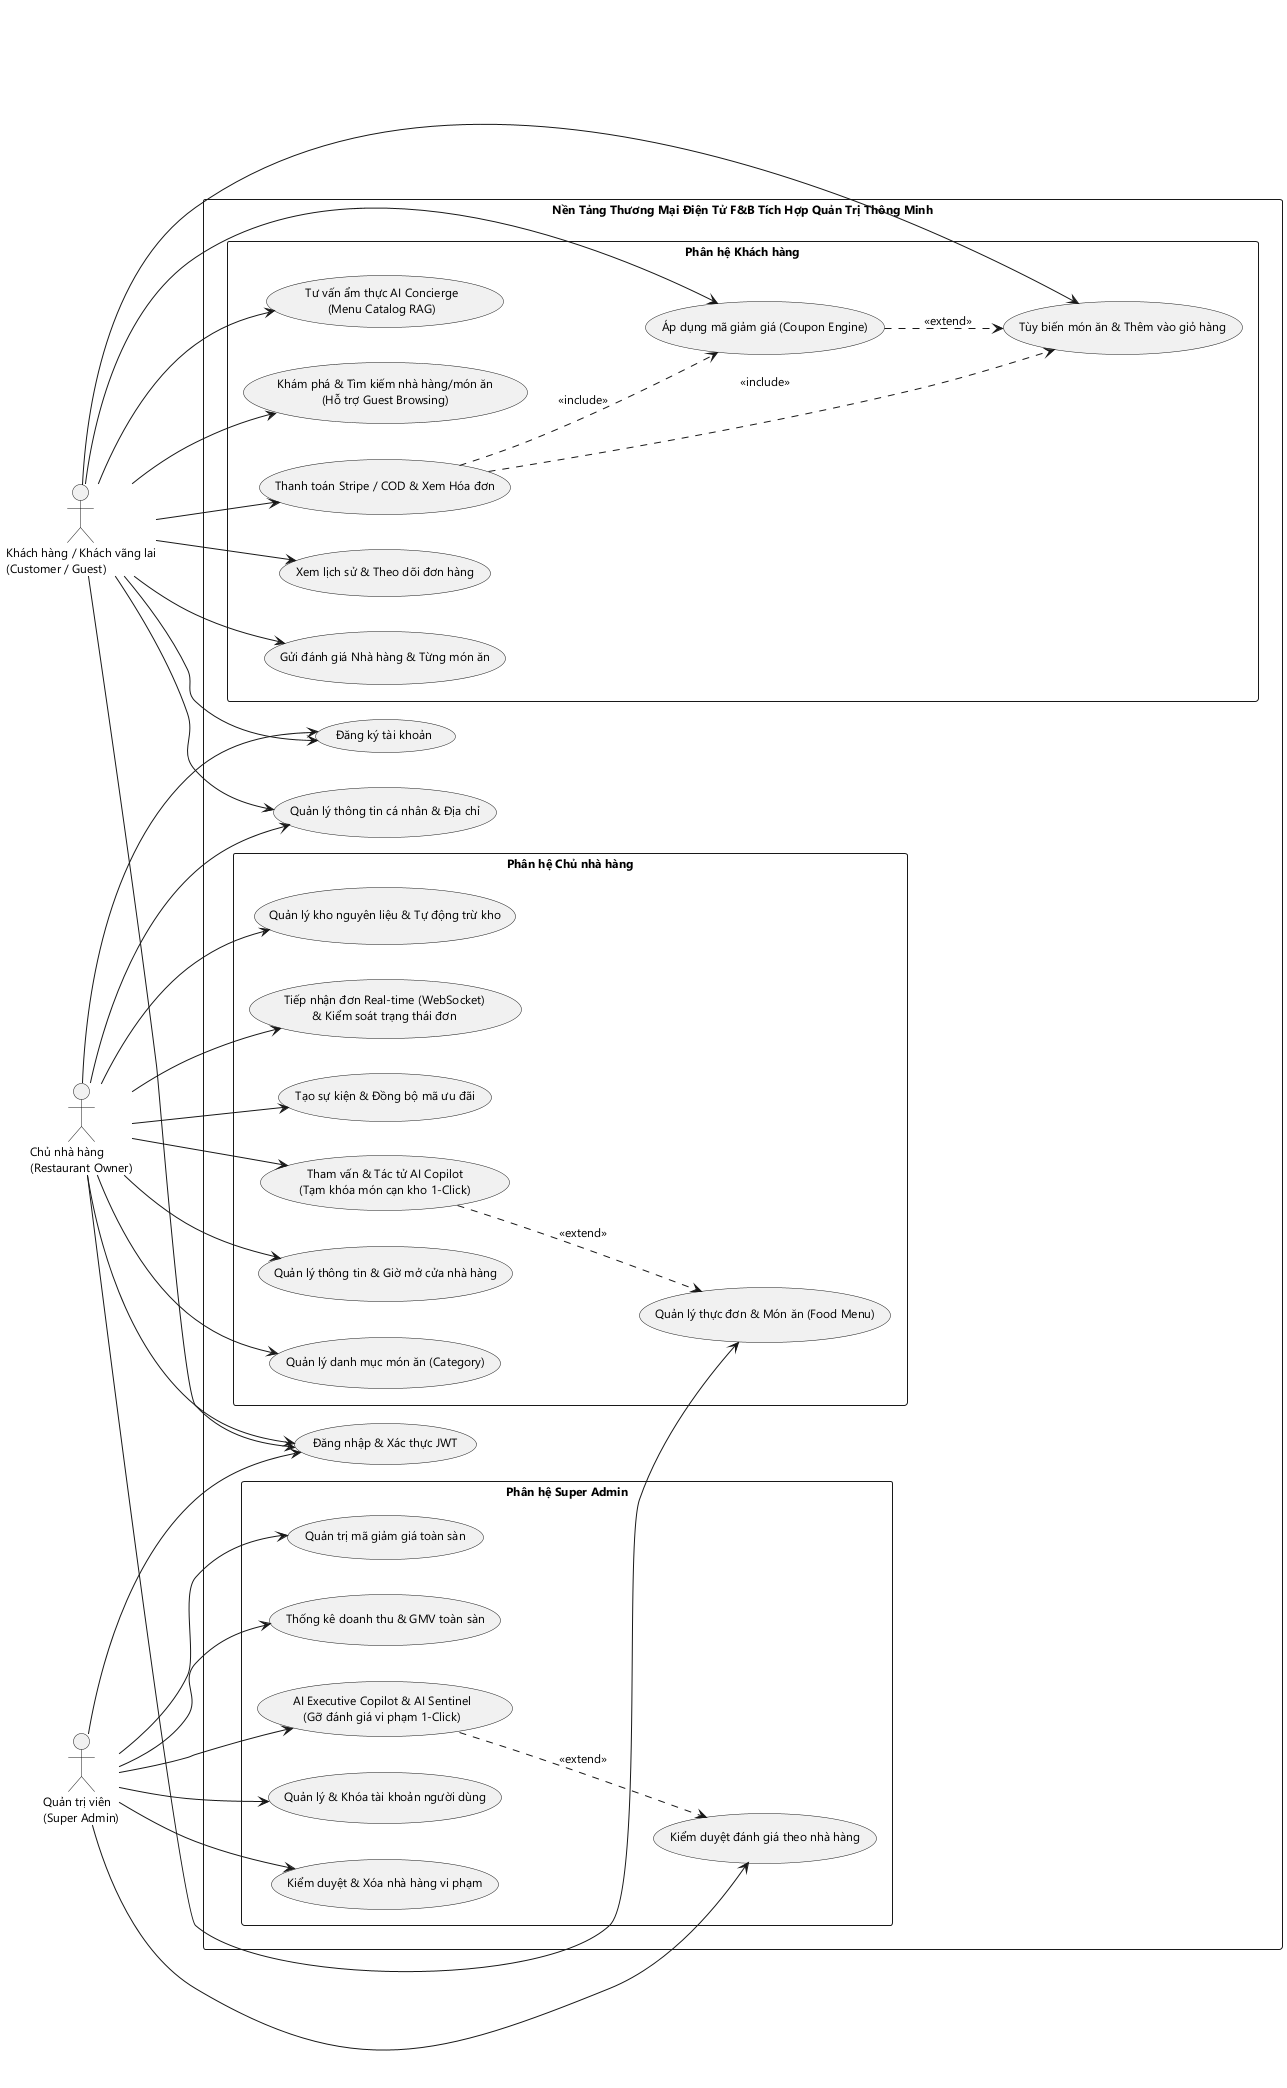
\includegraphics[width=0.95\textwidth]{figures/fig_usecase_general.png}
\end{figure}

Biểu đồ Hình 3.1 thể hiện rõ ba nhóm tác nhân chính của hệ thống là Khách hàng/Khách vãng lai (Customer/Guest), Chủ nhà hàng (Restaurant Owner) và Quản trị viên sàn (Super Admin), bao quát đầy đủ cả các ca sử dụng AI hiện đại như AI Concierge Menu RAG, Tác tử AI khóa món cạn kho và AI Sentinel kiểm duyệt.

\section{Đặc tả Chi tiết các Ca sử dụng Tiêu biểu}
Dưới đây là các bảng đặc tả chi tiết cho 11 ca sử dụng quan trọng nhất trong hệ thống, tuân thủ đúng định dạng chuẩn mực của khóa luận tốt nghiệp ngành Công nghệ thông tin.

% --- UC 1 ---
\subsection{Đặc tả Ca sử dụng: Đăng ký tài khoản}
\begin{table}{Phân tích ca sử dụng Đăng ký tài khoản}
\centering
\small
\begin{tabularx}{\textwidth}{|l|X|}
\hline
\textbf{Tên ca sử dụng} & \textbf{Đăng ký tài khoản mới (Signup with Role Sanitization)} \\ \hline
\textbf{Mã ca sử dụng} & UC-01 \\ \hline
\textbf{Tác nhân} & Khách hàng, Chủ nhà hàng mới \\ \hline
\textbf{Mô tả} & Cho phép người dùng mới tạo tài khoản trong hệ thống với vai trò Khách hàng hoặc Chủ nhà hàng, đồng thời tự động khởi tạo giỏ hàng trống và cấp phát JWT. \\ \hline
\textbf{Tiền điều kiện} & Người dùng truy cập trang web và chưa đăng nhập vào hệ thống. \\ \hline
\textbf{Hậu điều kiện} & Tài khoản người dùng mới được lưu vào CSDL; giỏ hàng trống được gán cho người dùng; mã JWT được trả về và lưu ở trình duyệt. \\ \hline
\textbf{Luồng cơ bản} & 
1. Người dùng mở hộp thoại Đăng nhập/Đăng ký trên thanh điều hướng.\newline
2. Người dùng chọn tab Đăng ký và điền Họ tên, Email, Mật khẩu, chọn vai trò (Khách hàng hoặc Chủ nhà hàng).\newline
3. Người dùng nhấn nút ``Đăng ký''.\newline
4. Hệ thống kiểm tra xem email đã được đăng ký trong hệ thống trước đó chưa.\newline
5. Hệ thống xác minh vai trò được yêu cầu có hợp lệ hay không (không được phép là ROLE\_ADMIN).\newline
6. Hệ thống mã hóa mật khẩu bằng thuật toán BCrypt.\newline
7. Hệ thống lưu bản ghi User vào CSDL và tự động tạo mới một Cart trống gắn với User đó.\newline
8. Hệ thống sinh mã JWT và trả về thông tin đăng nhập thành công kèm vai trò.\newline
9. Phía Client lưu JWT vào localStorage và tự động điều hướng người dùng. \\ \hline
\textbf{Luồng thay thế} & 
4a. Email đã tồn tại trong CSDL: Hệ thống trả về thông báo lỗi ``Email is already used with another account''; yêu cầu người dùng sử dụng email khác.\newline
5a. Người dùng cố tình gửi vai trò ROLE\_ADMIN qua API: Hệ thống từ chối yêu cầu và trả về lỗi ``Registration as ADMIN is not allowed.'' \\ \hline
\textbf{Luồng ngoại lệ} & 
Lỗi mất kết nối CSDL: Hệ thống hiển thị thông báo lỗi máy chủ và yêu cầu người dùng thử lại sau. \\ \hline
\end{tabularx}
\end{table}

% --- UC 2 ---
\subsection{Đặc tả Ca sử dụng: Đăng nhập tài khoản}
\begin{table}{Phân tích ca sử dụng Đăng nhập tài khoản}
\centering
\small
\begin{tabularx}{\textwidth}{|l|X|}
\hline
\textbf{Tên ca sử dụng} & \textbf{Đăng nhập tài khoản (Signin \& JWT Issuance)} \\ \hline
\textbf{Mã ca sử dụng} & UC-02 \\ \hline
\textbf{Tác nhân} & Khách hàng, Chủ nhà hàng, Quản trị viên Super Admin \\ \hline
\textbf{Mô tả} & Cho phép người dùng đăng nhập bằng Email và Mật khẩu, xác thực thông tin và cấp phát mã truy cập JWT. \\ \hline
\textbf{Tiền điều kiện} & Người dùng đã có tài khoản được khởi tạo trong CSDL. \\ \hline
\textbf{Hậu điều kiện} & Người dùng được xác thực danh tính; JWT được lưu trữ; giao diện cập nhật trạng thái đăng nhập. \\ \hline
\textbf{Luồng cơ bản} & 
1. Người dùng mở modal đăng nhập và nhập Email, Mật khẩu.\newline
2. Người dùng nhấn nút ``Đăng nhập''.\newline
3. Hệ thống tìm kiếm tài khoản theo Email và so khớp mật khẩu băm với BCrypt.\newline
4. Hệ thống nạp quyền hạn (Authorities) của người dùng vào Spring SecurityContext.\newline
5. Hệ thống sinh mã JWT có thời hạn và trả về Client kèm vai trò người dùng.\newline
6. Phía Client lưu JWT, gọi API lấy thông tin người dùng và giỏ hàng, cập nhật Store Redux.\newline
7. Hệ thống chuyển hướng người dùng đến trang phù hợp với quyền hạn. \\ \hline
\textbf{Luồng thay thế} & 
3a. Sai email hoặc mật khẩu: Hệ thống ném ngoại lệ \texttt{BadCredentialsException}, trả về mã lỗi 401 kèm thông báo ``Mật khẩu hoặc tài khoản không chính xác''. \\ \hline
\textbf{Luồng ngoại lệ} & 
Lỗi kết nối mạng: Giao diện hiển thị thông báo không thể kết nối tới máy chủ. \\ \hline
\end{tabularx}
\end{table}

% --- UC 3 ---
\subsection{Đặc tả Ca sử dụng: Quản lý giỏ hàng và Tùy biến món ăn}
\begin{table}{Phân tích ca sử dụng Quản lý giỏ hàng và tùy biến món ăn}
\centering
\small
\begin{tabularx}{\textwidth}{|l|X|}
\hline
\textbf{Tên ca sử dụng} & \textbf{Tùy biến món ăn \& Quản lý giỏ hàng} \\ \hline
\textbf{Mã ca sử dụng} & UC-03 \\ \hline
\textbf{Tác nhân} & Khách hàng \\ \hline
\textbf{Mô tả} & Khách hàng lựa chọn món ăn kèm các nguyên liệu tùy thích, thêm vào giỏ hàng, cập nhật số lượng hoặc xóa món. \\ \hline
\textbf{Tiền điều kiện} & Khách hàng đã đăng nhập tài khoản vào hệ thống. \\ \hline
\textbf{Hậu điều kiện} & Giỏ hàng của người dùng trên CSDL được cập nhật chính xác các món và tổng tiền tạm tính. \\ \hline
\textbf{Luồng cơ bản} & 
1. Khách hàng xem danh sách món ăn của một nhà hàng.\newline
2. Khách hàng nhấn vào món ăn, giao diện mở hộp thoại cho phép chọn thêm nguyên liệu (Ingredients: thêm phô mai, cay vừa, thêm thịt...).\newline
3. Khách hàng nhấn ``Thêm vào giỏ hàng''.\newline
4. Hệ thống kiểm tra xem món ăn có sẵn hàng không (\texttt{available == true}).\newline
5. Hệ thống thêm một \texttt{CartItem} mới vào giỏ hàng với danh sách nguyên liệu đã chọn.\newline
6. Hệ thống tính toán lại tổng tiền tạm tính của giỏ hàng và lưu vào bảng \texttt{cart}.\newline
7. Giao diện cập nhật biểu tượng giỏ hàng và thông báo món đã được thêm thành công. \\ \hline
\textbf{Luồng thay thế} & 
4a. Món ăn đã hết hàng: Hệ thống từ chối thao tác và hiển thị cảnh báo món hiện không khả dụng.\newline
5a. Khách hàng điều chỉnh số lượng (+/-) hoặc nhấn nút xóa món trong màn hình Giỏ hàng: Hệ thống cập nhật \texttt{CartItem} tương ứng và tính lại tổng tiền. \\ \hline
\textbf{Luồng ngoại lệ} & 
Món ăn bị chủ quán gỡ bỏ khỏi thực đơn trong lúc thao tác: Hệ thống cập nhật lại danh sách và báo lỗi cho khách hàng. \\ \hline
\end{tabularx}
\end{table}

% --- UC 4 ---
\subsection{Đặc tả Ca sử dụng: Áp dụng mã giảm giá ràng buộc}
\begin{table}{Phân tích ca sử dụng Áp dụng mã giảm giá ràng buộc}
\centering
\small
\begin{tabularx}{\textwidth}{|l|X|}
\hline
\textbf{Tên ca sử dụng} & \textbf{Áp dụng mã giảm giá ràng buộc (Coupon Constraint Engine)} \\ \hline
\textbf{Mã ca sử dụng} & UC-04 \\ \hline
\textbf{Tác nhân} & Khách hàng \\ \hline
\textbf{Mô tả} & Khách hàng nhập hoặc lựa chọn mã ưu đãi trong giỏ hàng; hệ thống thẩm định điều kiện ngưỡng giá trị tối thiểu, tính toán số tiền chiết khấu và tự động gỡ mã nếu không còn đủ điều kiện. \\ \hline
\textbf{Tiền điều kiện} & Giỏ hàng có ít nhất một món ăn và người dùng đang ở trang Giỏ hàng. \\ \hline
\textbf{Hậu điều kiện} & Mã giảm giá được áp dụng hợp lệ, hiển thị số tiền được giảm và tổng thanh toán mới. \\ \hline
\textbf{Luồng cơ bản} & 
1. Khách hàng nhập mã (ví dụ: \texttt{GIAM10\%}) hoặc click nút ``Áp dụng'' từ danh sách mã khả dụng.\newline
2. Giao diện mã hóa URL (\texttt{encodeURIComponent}) và gửi yêu cầu thẩm định tới Backend: \texttt{/api/coupons/validate}.\newline
3. Hệ thống tìm kiếm mã trong CSDL, kiểm tra trạng thái kích hoạt (\texttt{active == true}).\newline
4. Hệ thống tính toán tổng tiền các món thuộc phạm vi áp dụng (theo từng nhà hàng hoặc toàn sàn).\newline
5. Hệ thống so sánh tổng tiền này với giá trị đơn hàng tối thiểu (\texttt{minimumOrderValue}).\newline
6. Nếu thỏa mãn điều kiện, hệ thống tính toán số tiền giảm (theo \% hoặc số tiền cố định) với logic chặn biên \texttt{Math.max(0, Math.min(discount, applicableTotal))}.\newline
7. Giao diện hiển thị huy hiệu mã đã áp dụng thành công và cập nhật số tiền chiết khấu. \\ \hline
\textbf{Luồng thay thế} & 
3a. Mã không tồn tại hoặc hết hiệu lực: Báo lỗi ``Mã giảm giá không hợp lệ hoặc đã hết hạn''.\newline
5a. Tổng tiền chưa đạt ngưỡng tối thiểu: Báo lỗi ``Đơn hàng chưa đạt giá trị tối thiểu để áp dụng mã''.\newline
6a. Khách hàng giảm số lượng món khiến tổng tiền rơi xuống dưới ngưỡng tối thiểu: Cơ chế \textbf{Auto-removal} tại Client tự động gỡ bỏ mã và thông báo cho người dùng. \\ \hline
\textbf{Luồng ngoại lệ} & 
Lỗi cú pháp ký tự đặc biệt trong mã: Đã được xử lý triệt để thông qua Query Parameter và URL Encoding. \\ \hline
\end{tabularx}
\end{table}

% --- UC 5 ---
\subsection{Đặc tả Ca sử dụng: Thanh toán Đa phương thức (Stripe Checkout \& COD)}
\begin{table}{Phân tích ca sử dụng Thanh toán qua Stripe Checkout và COD}
\centering
\small
\begin{tabularx}{\textwidth}{|l|X|}
\hline
\textbf{Tên ca sử dụng} & \textbf{Thanh toán Đa phương thức (Stripe Checkout \& COD)} \\ \hline
\textbf{Mã ca sử dụng} & UC-05 \\ \hline
\textbf{Tác nhân} & Khách hàng, Cổng thanh toán Stripe \\ \hline
\textbf{Mô tả} & Khách hàng xác nhận thông tin đơn hàng, lựa chọn thanh toán trực tuyến qua cổng quốc tế Stripe hoặc tiền mặt khi nhận hàng (COD) và theo dõi hóa đơn điện tử. \\ \hline
\textbf{Tiền điều kiện} & Khách hàng đã chọn địa chỉ giao hàng và có sản phẩm trong giỏ hàng. \\ \hline
\textbf{Hậu điều kiện} & Đơn hàng lưu với \texttt{paymentMethod} tương ứng (\texttt{STRIPE} hoặc \texttt{COD}); đối với Stripe sau khi quẹt thẻ hoàn tất trạng thái chuyển thành \texttt{PAID}; giỏ hàng được làm sạch. \\ \hline
\textbf{Luồng cơ bản} & 
1. Khách hàng chọn phương thức thanh toán (\texttt{STRIPE} hoặc \texttt{COD}) tại màn hình Giỏ hàng và nhấn Đặt hàng.\newline
2. Hệ thống tạo bản ghi \texttt{Order} ở trạng thái \texttt{PENDING} kèm \texttt{paymentMethod}, thực thi khấu trừ kho tự động và gửi thông báo WebSocket tới nhà hàng.\newline
3. Nếu chọn Stripe: Hệ thống gọi Stripe SDK tạo Session thanh toán theo số tiền thực tế (đã trừ khuyến mãi) và chuyển hướng khách tới Stripe Checkout.\newline
4. Khách hàng nhập thông tin thẻ hợp lệ và xác nhận thanh toán.\newline
5. Stripe xử lý giao dịch thành công và chuyển hướng người dùng về \texttt{/payment/success/:id}.\newline
6. Phía Client kích hoạt API callback \texttt{PUT /api/order/\{id\}/complete-payment} (đã mở khóa \texttt{permitAll} an toàn).\newline
7. Máy chủ cập nhật trạng thái đơn hàng thành \texttt{PAID} và hiển thị giao diện xác nhận kèm liên kết xuất hóa đơn điện tử. \\ \hline
\textbf{Luồng thay thế} & 
1a. Khách hàng chọn thanh toán \texttt{COD}: Máy chủ trả về \texttt{payment\_url = null}; ứng dụng chuyển thẳng sang trang Lịch sử đơn hàng (\texttt{/my-profile/orders}) ở trạng thái \texttt{PENDING} chờ quán xác nhận.\newline
4a. Khách hàng hủy trên giao diện Stripe: Stripe chuyển hướng về \texttt{/payment/fail}; đơn hàng giữ trạng thái \texttt{PENDING} và khách có thể bấm ``Thanh toán ngay'' lại sau. \\ \hline
\textbf{Luồng ngoại lệ} & 
Mất kết nối hoặc token hết hạn khi Stripe redirect: Nhờ mở khóa endpoint \texttt{complete-payment}, trạng thái thanh toán của đơn vẫn được ghi nhận chính xác, đồng thời chủ quán vẫn có nút ``Xác nhận đã thanh toán'' dự phòng. \\ \hline
\end{tabularx}
\end{table}

% --- UC 6 ---
\subsection{Đặc tả Ca sử dụng: Quản lý thực đơn và kho nguyên liệu}
\begin{table}{Phân tích ca sử dụng Quản lý thực đơn và nguyên liệu}
\centering
\small
\begin{tabularx}{\textwidth}{|l|X|}
\hline
\textbf{Tên ca sử dụng} & \textbf{Quản lý thực đơn \& Kho nguyên liệu của nhà hàng} \\ \hline
\textbf{Mã ca sử dụng} & UC-06 \\ \hline
\textbf{Tác nhân} & Chủ nhà hàng (Restaurant Owner) \\ \hline
\textbf{Mô tả} & Cho phép chủ quán thêm, sửa, xóa món ăn, thiết lập giá bán, cập nhật trạng thái còn/hết hàng và quản lý phân loại các nguyên liệu thành phần. \\ \hline
\textbf{Tiền điều kiện} & Chủ nhà hàng đã đăng nhập và sở hữu một nhà hàng trên hệ thống. \\ \hline
\textbf{Hậu điều kiện} & Thông tin thực đơn và nguyên liệu được cập nhật tức thời trên CSDL và hiển thị cho thực khách. \\ \hline
\textbf{Luồng cơ bản} & 
1. Chủ nhà hàng truy cập trang quản trị nhà hàng và chọn mục ``Menu'' hoặc ``Ingredients''.\newline
2. Để thêm món ăn mới: Chủ quán nhấn ``Tạo món mới'', nhập tên món, mô tả, giá tiền, chọn danh mục, gán các nhóm nguyên liệu và tải lên hình ảnh món ăn.\newline
3. Chủ quán nhấn nút ``Lưu món ăn''.\newline
4. Hệ thống kiểm tra quyền sở hữu nhà hàng và lưu bản ghi món ăn vào bảng \texttt{food}.\newline
5. Để cập nhật trạng thái còn/hết hàng: Chủ quán gạt nút chuyển trạng thái tại dòng món ăn hoặc nguyên liệu tương ứng.\newline
6. Hệ thống thực hiện cập nhật trường \texttt{available} (đối với món ăn) hoặc \texttt{inStock} (đối với nguyên liệu) trong CSDL. \\ \hline
\textbf{Luồng thay thế} & 
4a. Dữ liệu nhập vào bị thiếu trường bắt buộc (ví dụ: giá âm, tên trống): Hệ thống hiển thị cảnh báo lỗi nhập liệu tại form. \\ \hline
\textbf{Luồng ngoại lệ} & 
Chủ quán chưa tạo hồ sơ nhà hàng: Hệ thống tự động chuyển hướng chủ quán về màn hình khởi tạo nhà hàng (\texttt{CreateRestaurantForm}). \\ \hline
\end{tabularx}
\end{table}

% --- UC 7 ---
\subsection{Đặc tả Ca sử dụng: Tiếp nhận và Kiểm soát Máy trạng thái Đơn hàng}
\begin{table}{Phân tích ca sử dụng Tiếp nhận và kiểm soát máy trạng thái đơn hàng}
\centering
\small
\begin{tabularx}{\textwidth}{|l|X|}
\hline
\textbf{Tên ca sử dụng} & \textbf{Tiếp nhận \& Kiểm soát Máy trạng thái Đơn hàng (Order Fulfillment)} \\ \hline
\textbf{Mã ca sử dụng} & UC-07 \\ \hline
\textbf{Tác nhân} & Chủ nhà hàng \\ \hline
\textbf{Mô tả} & Chủ quán xem danh sách đơn hàng được sắp xếp mới nhất lên đầu kèm phương thức thanh toán, theo dõi chi tiết món ăn và điều phối chuyển đổi trạng thái hợp lệ. \\ \hline
\textbf{Tiền điều kiện} & Chủ quán đăng nhập vào Bảng điều khiển quản trị nhà hàng. \\ \hline
\textbf{Hậu điều kiện} & Trạng thái đơn hàng tuân thủ Máy trạng thái đơn hàng; tự động hoàn kho nếu hủy đơn và phát sóng WebSocket. \\ \hline
\textbf{Luồng cơ bản} & 
1. Chủ quán chọn mục ``Đơn hàng'' trên thanh menu quản trị.\newline
2. Hệ thống truy vấn \texttt{/api/admin/order/restaurant/\{id\}} (đã sắp xếp \texttt{ORDER BY createdAt DESC, id DESC}).\newline
3. Bảng hiển thị danh sách đơn kèm huy hiệu thanh toán (\texttt{STRIPE} / \texttt{COD}) và trạng thái hiện tại.\newline
4. Chủ quán chọn chuyển trạng thái tuần tự (\texttt{PAID} $\to$ \texttt{OUT\_FOR\_DELIVERY} $\to$ \texttt{COMPLETED} hoặc \texttt{CANCELLED}).\newline
5. Hệ thống gọi API \texttt{PUT /api/admin/order/\{orderId\}/\{orderStatus\}}.\newline
6. Máy chủ áp dụng \textbf{Order State Guard}: kiểm tra quyền sở hữu và tính hợp lệ của bước chuyển trạng thái, sau đó lưu CSDL và phát sóng sự kiện \texttt{STATUS\_UPDATED}. \\ \hline
\textbf{Luồng thay thế} & 
4a. Chủ quán hủy đơn (\texttt{CANCELLED}): Hệ thống tự động kích hoạt \texttt{restoreStockForOrder(order)} để hoàn trả nguyên liệu vào kho và ghi log \texttt{AUTO\_RESTORE}. \\ \hline
\textbf{Luồng ngoại lệ} & 
6a. Cố tình sửa đơn đã kết thúc (\texttt{COMPLETED}/\texttt{CANCELLED}) hoặc chuyển đơn Stripe \texttt{PENDING} nhảy cóc sang \texttt{OUT\_FOR\_DELIVERY}: Hệ thống chặn và ném ngoại lệ bảo vệ nghiệp vụ. \\ \hline
\end{tabularx}
\end{table}

% --- UC 8 ---
\subsection{Đặc tả Ca sử dụng: Kiểm duyệt đánh giá và Quản trị toàn sàn}
\begin{table}{Phân tích ca sử dụng Kiểm duyệt đánh giá và Quản trị sàn}
\centering
\small
\begin{tabularx}{\textwidth}{|l|X|}
\hline
\textbf{Tên ca sử dụng} & \textbf{Kiểm duyệt đánh giá \& Quản trị toàn sàn của Super Admin} \\ \hline
\textbf{Mã ca sử dụng} & UC-08 \\ \hline
\textbf{Tác nhân} & Quản trị viên tối cao (Super Admin) \\ \hline
\textbf{Mô tả} & Quản trị viên theo dõi các chỉ số tổng thể, kiểm duyệt và xóa các bài đánh giá vi phạm chuẩn mực, loại bỏ các nhà hàng không đạt tiêu chuẩn. \\ \hline
\textbf{Tiền điều kiện} & Người dùng đăng nhập thành công với tài khoản có vai trò \texttt{ROLE\_ADMIN}. \\ \hline
\textbf{Hậu điều kiện} & Đánh giá hoặc nhà hàng vi phạm bị loại bỏ vĩnh viễn khỏi CSDL. \\ \hline
\textbf{Luồng cơ bản} & 
1. Super Admin đăng nhập và truy cập phân hệ quản trị toàn sàn.\newline
2. Admin chọn mục ``Reviews'' để xem toàn bộ đánh giá của khách hàng trên toàn bộ các món ăn và nhà hàng.\newline
3. Admin phát hiện một bài đánh giá có ngôn từ phản cảm hoặc mang tính spam phá hoại.\newline
4. Admin nhấn nút ``Xóa đánh giá vi phạm''.\newline
5. Hệ thống gửi yêu cầu \texttt{DELETE /api/admin/reviews/\{reviewId\}} kèm mã JWT của Admin.\newline
6. Máy chủ xác thực quyền \texttt{ROLE\_ADMIN}, thực thi thao tác xóa bản ghi trong bảng \texttt{review}.\newline
7. Hệ thống cập nhật lại danh sách đánh giá và tính toán lại điểm số sao trung bình của món ăn.\newline
8. Admin nhận được thông báo đã gỡ bỏ thành công đánh giá vi phạm. \\ \hline
\textbf{Luồng thay thế} & 
3a. Admin phát hiện nhà hàng có dấu hiệu gian lận: Admin vào mục Quản trị nhà hàng và nhấn ``Xóa nhà hàng''; hệ thống xác nhận và thực hiện vô hiệu hóa/xóa nhà hàng đó khỏi hệ thống. \\ \hline
\textbf{Luồng ngoại lệ} & 
Tài khoản không phải ROLE\_ADMIN cố tình gọi API kiểm duyệt: Spring Security chặn ngay lập tức với mã lỗi 403 Forbidden. \\ \hline
\end{tabularx}
\end{table}

% --- UC 9 ---
\subsection{Đặc tả Ca sử dụng: Tham vấn \& Thực thi Tác tử Hành động AI Copilot}
\begin{table}{Phân tích ca sử dụng Tham vấn và thực thi Tác tử AI Copilot}
\centering
\small
\begin{tabularx}{\textwidth}{|l|X|}
\hline
\textbf{Tên ca sử dụng} & \textbf{Tham vấn Quản trị \& Thực thi Tác tử AI Hành động (Dual-Persona Agentic AI)} \\ \hline
\textbf{Mã ca sử dụng} & UC-09 \\ \hline
\textbf{Tác nhân} & Chủ nhà hàng (Restaurant Owner), Quản trị viên Sàn (Super Admin) \\ \hline
\textbf{Mô tả} & Cho phép Chủ quán và Super Admin tra cứu chỉ số vận hành theo thời gian thực, nhận phân tích chiến lược từ Google Gemini 2.5 Flash (hoặc Heuristic DSS dự phòng) kèm thẻ hành động tự động 1-Click. \\ \hline
\textbf{Tiền điều kiện} & Người dùng đã đăng nhập với vai trò \texttt{ROLE\_RESTAURANT\_OWNER} hoặc \texttt{ROLE\_ADMIN}. \\ \hline
\textbf{Hậu điều kiện} & Hiển thị 4 thẻ KPI theo vai trò, phản hồi Markdown và thẻ đề xuất hành động (\texttt{agentAction}) sẵn sàng thực thi xuống CSDL. \\ \hline
\textbf{Luồng cơ bản} & 
1. Người quản trị chọn mục ``Trợ lý AI Copilot'' trên thanh điều hướng.\newline
2. Giao diện tự động gọi \texttt{GET /api/admin/ai/copilot/quick-insights/\{id\}} (với \texttt{0} cho Super Admin) và hiển thị 4 thẻ KPI tương ứng vai trò.\newline
3. Người quản trị nhập câu hỏi hoặc bấm câu hỏi gợi ý (ví dụ: Chủ quán chọn ``Cảnh báo nguyên liệu sắp hết''; Super Admin chọn ``Kiểm duyệt bình luận độc hại'').\newline
4. Hệ thống gửi \texttt{POST /api/admin/ai/copilot/chat}.\newline
5. Backend tổng hợp số liệu từ DB, gọi Google Gemini 2.5 Flash (hoặc kích hoạt Heuristic DSS dự phòng) và gọi \texttt{determineAgentAction()} để sinh gói \texttt{agentAction}.\newline
6. Phía Client hiển thị báo cáo Markdown kèm thẻ \textbf{Tác tử AI Hành Động} tương tác.\newline
7. Người dùng bấm nút Tác tử AI: Hệ thống thực thi khóa món cạn kho (\texttt{PUT /api/admin/food/\{foodId\}}) hoặc gỡ bỏ đánh giá vi phạm (\texttt{DELETE /api/reviews/\{reviewId\}}). \\ \hline
\textbf{Luồng thay thế} & 
5a. Gemini API quá hạn hoặc chưa cấu hình Key: Động cơ Heuristic DSS phân tách vai trò (Owner DSS vs. AI Content Moderation Sentinel) lập tức trả về phân tích và \texttt{agentAction} trong dưới 5ms. \\ \hline
\textbf{Luồng ngoại lệ} & 
Lỗi quyền truy cập hoặc mất kết nối CSDL: Hệ thống thông báo lỗi rõ ràng trên khung hội thoại. \\ \hline
\end{tabularx}
\end{table}

% --- UC 10 ---
\subsection{Đặc tả Ca sử dụng: Cảnh báo Đơn hàng Thời gian thực và Trừ Kho Tự động}
\begin{table}{Phân tích ca sử dụng Cảnh báo đơn hàng thời gian thực và trừ kho tự động}
\centering
\small
\begin{tabularx}{\textwidth}{|l|X|}
\hline
\textbf{Tên ca sử dụng} & \textbf{Cảnh báo Đơn hàng Thời gian thực \& Quản lý Tồn kho Tự động} \\ \hline
\textbf{Mã ca sử dụng} & UC-10 \\ \hline
\textbf{Tác nhân} & Khách hàng (kích hoạt), Chủ nhà hàng (tiếp nhận), WebSocket Server \\ \hline
\textbf{Mô tả} & Khi khách hàng hoàn tất đặt đơn, hệ thống tự động khấu trừ định lượng nguyên liệu trong kho bếp và phát sóng thông báo đẩy qua kênh WebSocket kèm chuông báo tức thời đến màn hình quản trị của chủ quán. \\ \hline
\textbf{Tiền điều kiện} & Khách hàng thực hiện đặt đơn thành công; Chủ quán đang mở màn hình quản trị và duy trì kết nối WebSocket. \\ \hline
\textbf{Hậu điều kiện} & Số lượng nguyên liệu chế biến giảm tương ứng trong CSDL; bản ghi \texttt{InventoryLog} được lưu; đơn hàng mới xuất hiện ngay lập tức trên bảng điều khiển của chủ quán kèm chuông reo. \\ \hline
\textbf{Luồng cơ bản} & 
1. Khách hàng nhấn xác nhận đặt hàng tại màn hình thanh toán.\newline
2. Backend kiểm tra và lưu đơn hàng mới vào bảng \texttt{orders}.\newline
3. Phương thức \texttt{depleteStockForOrder} duyệt qua từng món trong đơn, lấy danh sách nguyên liệu thành phần và trừ số lượng tồn kho theo số lượng món đặt mua.\newline
4. Hệ thống ghi nhật ký xuất kho với hành động \texttt{AUTO\_DEPLETION} vào bảng \texttt{inventory\_log}. Nếu số lượng tồn kho về 0, hệ thống tự động đánh dấu \texttt{inStock = false}.\newline
5. Backend đóng gói thông tin đơn hàng thành đối tượng \texttt{OrderNotificationDTO} và gọi \texttt{broadcastToRestaurant}.\newline
6. WebSocket Server gửi tin nhắn JSON tới toàn bộ các kết nối đang mở của nhà hàng.\newline
7. Phía Client nhận gói tin qua \texttt{OrderNotificationListener.jsx}, kích hoạt hàm \texttt{playOrderChime()} tạo chuông 3 âm sắc (E5 $\to$ G\#5 $\to$ B5) qua Web Audio API và cập nhật danh sách đơn hàng mà không cần tải lại trang. \\ \hline
\textbf{Luồng thay thế} & 
2a. Đơn hàng sau đó bị khách hoặc chủ quán hủy (\texttt{CANCELLED}): Backend kích hoạt phương thức \texttt{restoreStockForOrder}, hoàn trả lại số lượng tồn kho nguyên liệu, ghi log \texttt{AUTO\_RESTORE} và gửi thông báo qua WebSocket để chủ quán dừng chuẩn bị món. \\ \hline
\textbf{Luồng ngoại lệ} & 
Kết nối WebSocket bị ngắt do mạng gián đoạn: Phía Frontend có cơ chế tự động kết nối lại (Auto-reconnect) định kỳ 3 giây một lần. \\ \hline
\end{tabularx}
\end{table}

% --- UC 11 ---
\subsection{Đặc tả Ca sử dụng: Tư vấn Ẩm thực Khách hàng (AI Concierge \& Menu RAG)}
\begin{table}{Phân tích ca sử dụng Tư vấn ẩm thực AI Concierge Menu Catalog RAG}
\centering
\small
\begin{tabularx}{\textwidth}{|l|X|}
\hline
\textbf{Tên ca sử dụng} & \textbf{Tư vấn Ẩm thực Khách hàng qua Trợ lý AI Concierge (Menu Catalog RAG)} \\ \hline
\textbf{Mã ca sử dụng} & UC-11 \\ \hline
\textbf{Tác nhân} & Khách hàng / Khách vãng lai (Customer / Guest) \\ \hline
\textbf{Mô tả} & Cho phép người dùng truy cập nền tảng tương tác với Widget Trợ lý Ẩm thực để được gợi ý món bán chạy thực tế, xem mã giảm giá hiệu lực và điều hướng trực tiếp tới đúng món ăn tại nhà hàng. \\ \hline
\textbf{Tiền điều kiện} & Người dùng mở giao diện khách hàng của nền tảng (không bắt buộc đăng nhập). \\ \hline
\textbf{Hậu điều kiện} & Khách hàng nhận được thẻ món ăn trực quan khớp ngữ cảnh thực tế từ DB và mở nhanh thực đơn tại món ăn được gợi ý. \\ \hline
\textbf{Luồng cơ bản} & 
1. Khi truy cập trang chủ, component \texttt{Chatbot.jsx} nạp sẵn ngữ cảnh thực tế từ \texttt{GET /api/food/popular} và \texttt{GET /api/coupons}.\newline
2. Người dùng bấm biểu tượng Chat nổi ở góc phải màn hình.\newline
3. Người dùng chọn câu hỏi gợi ý (VD: ``Gợi ý cơm trưa ngon hôm nay'') hoặc nhập từ khóa món ăn.\newline
4. Bộ truy xuất Menu Catalog RAG tìm kiếm món bán chạy phù hợp nhất kèm mã ưu đãi đang kích hoạt.\newline
5. Giao diện kết xuất thẻ món ăn giàu thông tin gồm ảnh thực tế, giá niêm yết, tên nhà hàng, mẹo nhập mã \texttt{GIAM20K} và nút ``Xem Quán \& Đặt Món Ngay''.\newline
6. Khách hàng bấm nút: hệ thống điều hướng tới \texttt{/restaurant/\{city\}/\{name\}/\{id\}?foodId=\{foodId\}}, tự động cuộn mượt và làm nổi bật (highlight) đúng món ăn đó. \\ \hline
\textbf{Luồng thay thế} & 
4a. Khách hàng hỏi về danh sách nhà hàng, mã giảm giá hoặc quy định hủy đơn/giao hàng: Chatbot trích xuất thông tin trực tiếp từ Redux Store và trả lời tức thời. \\ \hline
\textbf{Luồng ngoại lệ} & 
Backend tạm thời không tải được món phổ biến: Chatbot tự động chuyển sang món gợi ý dự phòng chuẩn (\textit{Cơm Sườn Cây Nướng Mật Ong}). \\ \hline
\end{tabularx}
\end{table}

% =========================================================================
% CHƯƠNG 4: PHÂN TÍCH VÀ THIẾT KẾ HỆ THỐNG
% =========================================================================
\chapter{PHÂN TÍCH VÀ THIẾT KẾ HỆ THỐNG}

\section{Kiến trúc Hệ thống Tổng thể và Sơ đồ Triển khai}
\subsection{Kiến trúc Phân tầng Logic của Hệ thống}
Hệ thống được thiết kế theo mô hình kiến trúc phân tầng 3 lớp (3-Tier Architecture) nhằm đảm bảo sự linh hoạt, dễ bảo trì và khả năng mở rộng trong tương lai:
\begin{enumerate}
    \item \textbf{Tầng Trình diễn (Client Layer):} Được xây dựng bằng React 19 chạy trên môi trường trình duyệt. Tầng này chịu trách nhiệm hiển thị giao diện, tiếp nhận thao tác người dùng, xử lý các kiểm tra nghiệp vụ tức thời ở phía máy khách (như kiểm tra ràng buộc mã giảm giá trước khi gửi request) và quản lý trạng thái bằng Redux Toolkit.
    \item \textbf{Tầng Ứng dụng \& Dịch vụ (Application \& Service Layer):} Được xây dựng trên Spring Boot 3.4.0 chạy Java 17, bao gồm:
    \begin{itemize}
        \item \textit{Security Filter Chain:} Chặn lọc và xác thực các token JWT đính kèm trong HTTP Header.
        \item \textit{Controller Layer:} Tiếp nhận các yêu cầu HTTP, kiểm tra tính hợp lệ của tham số đầu vào và chuyển tiếp tới tầng dịch vụ.
        \item \textit{Service Layer:} Nơi thực thi logic nghiệp vụ cốt lõi: xử lý đơn hàng, tính toán chiết khấu khuyến mãi an toàn, tương tác với Stripe SDK.
        \item \textit{Data Access Layer (Repository):} Sử dụng Spring Data JPA để tương tác và thực thi các câu lệnh truy vấn xuống CSDL MySQL.
    \end{itemize}
    \item \textbf{Tầng Dịch vụ Bên ngoài (External Cloud Services):} Bao gồm Cổng thanh toán quốc tế Stripe tiếp nhận giao dịch thẻ PCI DSS và \textbf{Google Cloud AI Services (Gemini 2.5 Flash LLM API)} phục vụ tư vấn vận hành chiến lược cho AI Copilot.
\end{enumerate}

\subsection{Sơ đồ Triển khai Hệ thống (Deployment Diagram)}
Sơ đồ vật lý triển khai các thành phần của hệ thống được mô tả trong Hình 4.1:

\begin{figure}{Sơ đồ Triển khai Vật lý của Hệ thống (Deployment Diagram)}
\centering
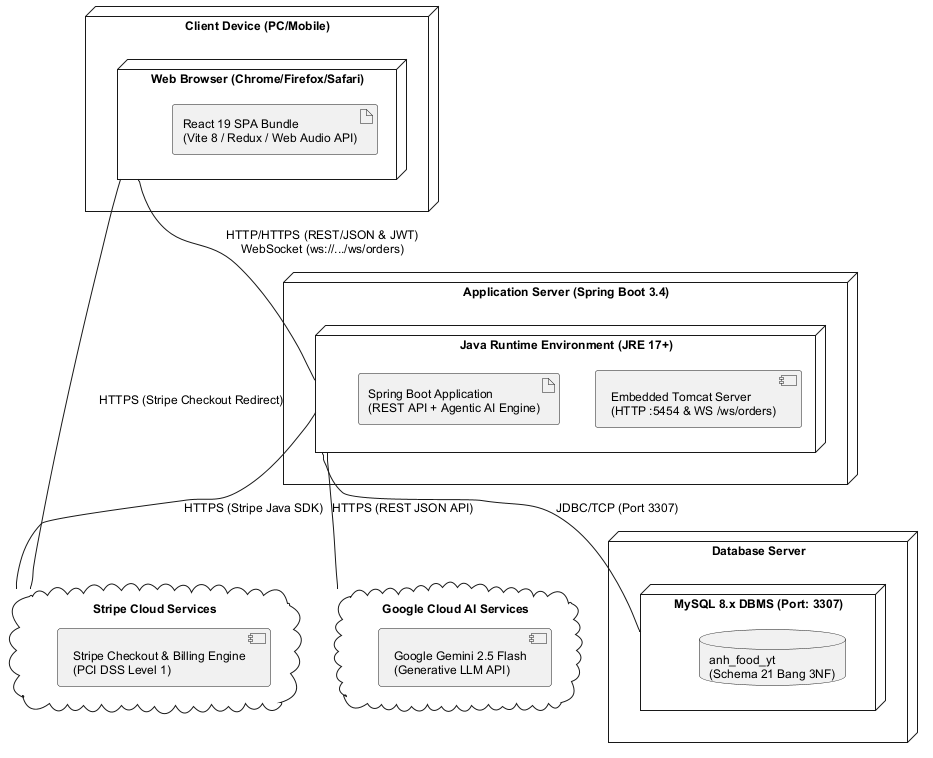
\includegraphics[width=0.88\textwidth]{figures/fig_deployment.png}
\end{figure}

Theo Hình 4.1, hệ thống bao gồm 5 khối kiến trúc vật lý chính:
\begin{itemize}
    \item \textbf{Khối Thiết bị Người dùng (Client Device):} Chạy trình duyệt web hiện đại (Chrome, Edge, Firefox, Safari) kết xuất gói bundle SPA của React 19 (Vite 8, Redux Toolkit, Web Audio API).
    \item \textbf{Khối Máy chủ Ứng dụng (Application Server - Spring Boot 3.4):} Môi trường chạy JRE 17+, triển khai file \texttt{.jar} Spring Boot với Embedded Tomcat lắng nghe giao thức HTTP REST và WebSocket (\texttt{/ws/orders}) trên cổng 5454 cùng Agentic AI Decision Engine.
    \item \textbf{Khối Máy chủ Cơ sở Dữ liệu (Database Server):} Hệ quản trị MySQL 8.x chạy trên cổng 3307, lưu trữ schema dữ liệu \texttt{anh\_food\_yt} gồm 21 bảng chuẩn 3NF.
    \item \textbf{Khối Dịch vụ Đám mây Stripe (Stripe Cloud Services):} Động cơ xử lý thanh toán Checkout Session chuẩn PCI DSS giao tiếp qua Stripe Java SDK.
    \item \textbf{Khối Dịch vụ AI Đám mây Google (Google Cloud AI Services):} Điểm cuối REST API \textbf{Google Gemini 2.5 Flash} kết nối qua HTTPS để tạo phân tích điều hành F\&B chuyên sâu.
\end{itemize}

\section{Biểu đồ Tuần tự cho các Luồng Nghiệp vụ Cốt lõi}
Phần này trình bày chi tiết các biểu đồ tuần tự (Sequence Diagrams) minh họa trực quan sự tương tác giữa các thành phần phần mềm trong hệ thống qua thời gian đối với các ca sử dụng tiêu biểu.

\subsection{Biểu đồ Tuần tự: Đăng ký \& Đăng nhập Phân quyền JWT}
Quy trình xác thực người dùng được mô tả trong Hình 4.2:

\begin{figure}{Biểu đồ tuần tự ca sử dụng Đăng ký và Đăng nhập xác thực JWT}
\centering
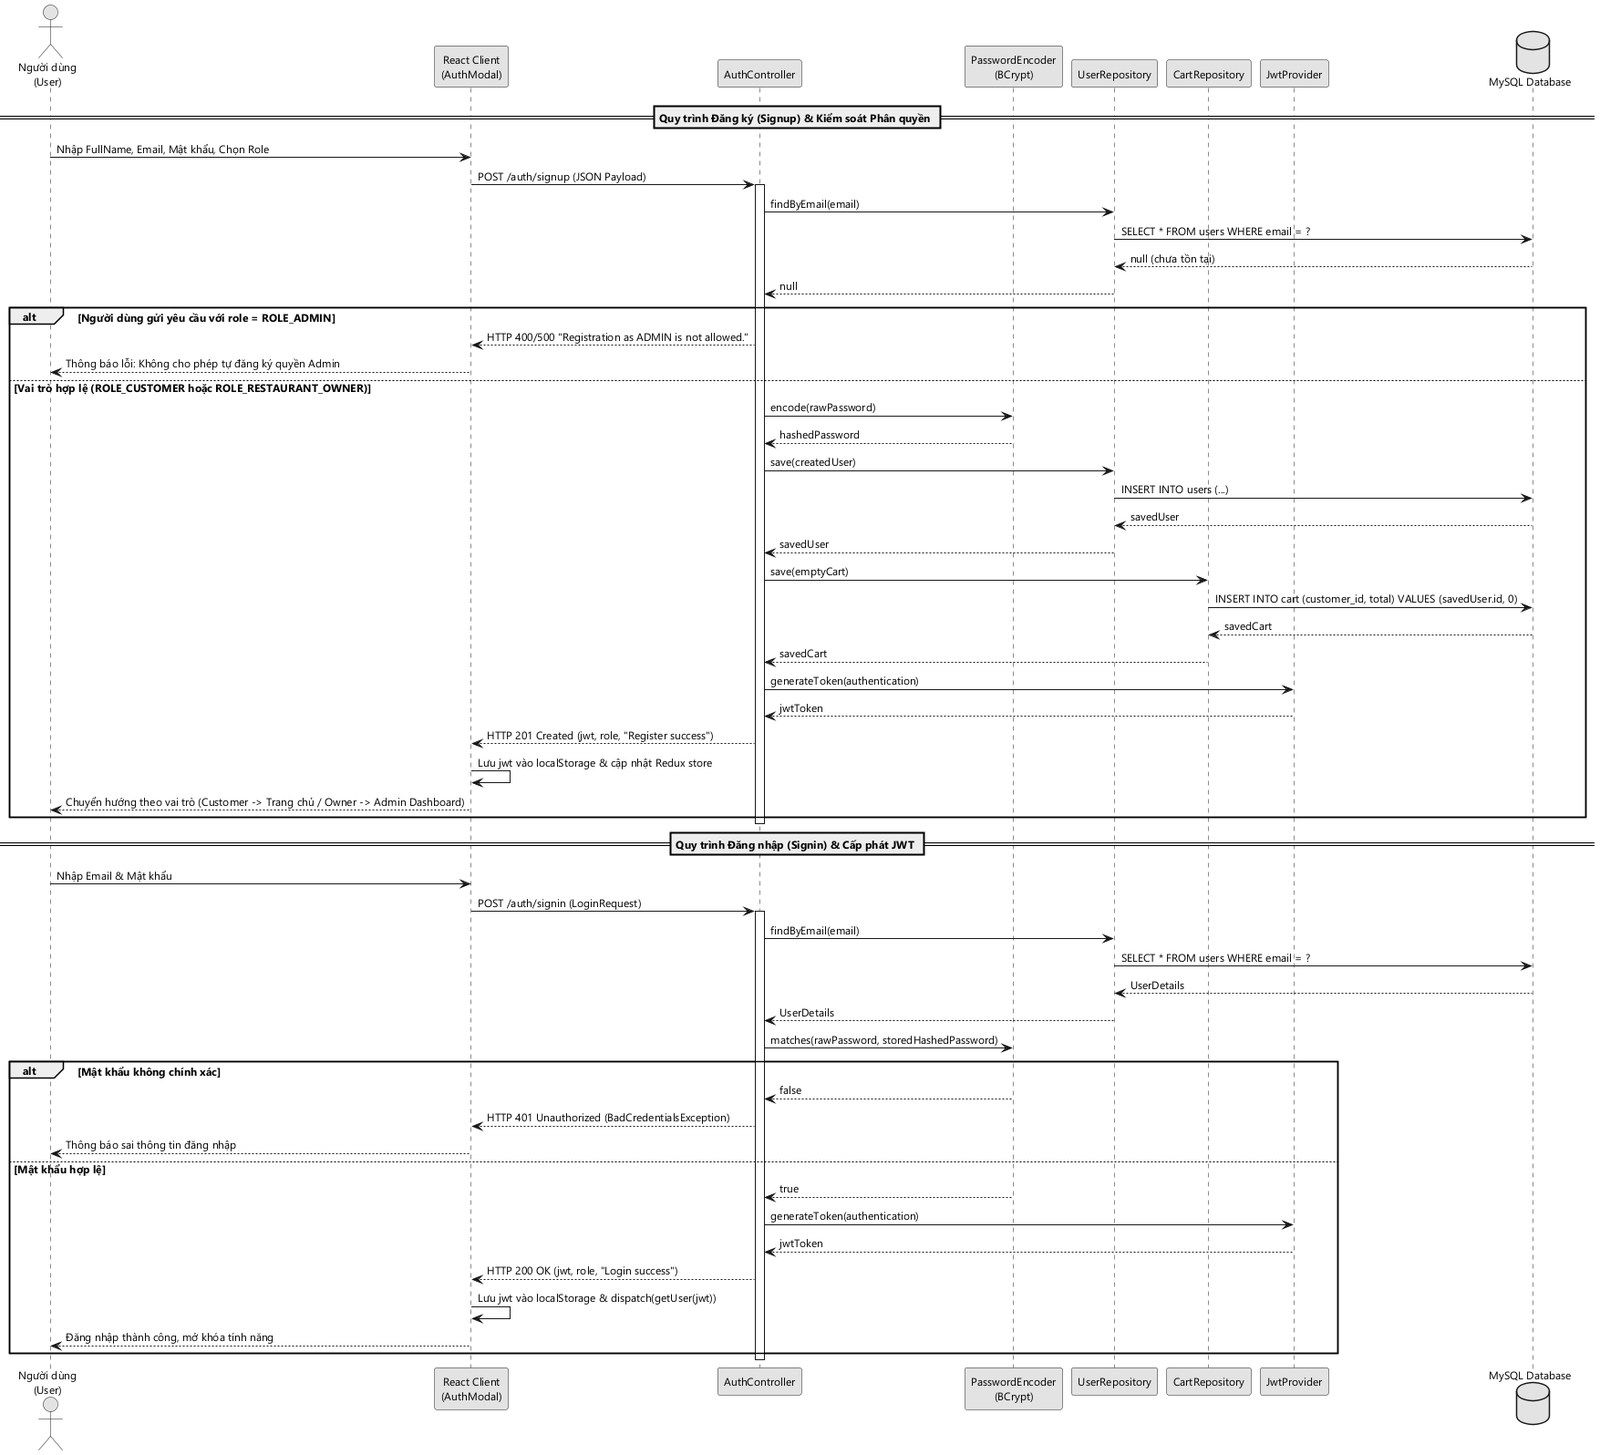
\includegraphics[width=0.92\textwidth]{figures/fig_sequence_auth.png}
\end{figure}

Sơ đồ Hình 4.2 thể hiện cơ chế bảo mật quan trọng: Khi người dùng gửi yêu cầu đăng ký qua API \texttt{/auth/signup}, Controller trước tiên sẽ kiểm tra nếu trường \texttt{role} có giá trị \texttt{ROLE\_ADMIN} thì ngay lập tức ném ra ngoại lệ từ chối, ngăn chặn mọi nỗ lực leo thang đặc quyền từ bên ngoài. Mật khẩu được băm một chiều qua BCrypt trước khi ghi vào CSDL, đồng thời một giỏ hàng trống mới được tạo tự động để người dùng sẵn sàng mua hàng.

\subsection{Biểu đồ Tuần tự: Giỏ hàng và Áp dụng Mã Giảm giá Ràng buộc}
Quy trình tính toán khuyến mãi thông minh được mô tả trong Hình 4.3:

\begin{figure}{Biểu đồ tuần tự ca sử dụng Giỏ hàng và Áp dụng mã giảm giá ràng buộc}
\centering
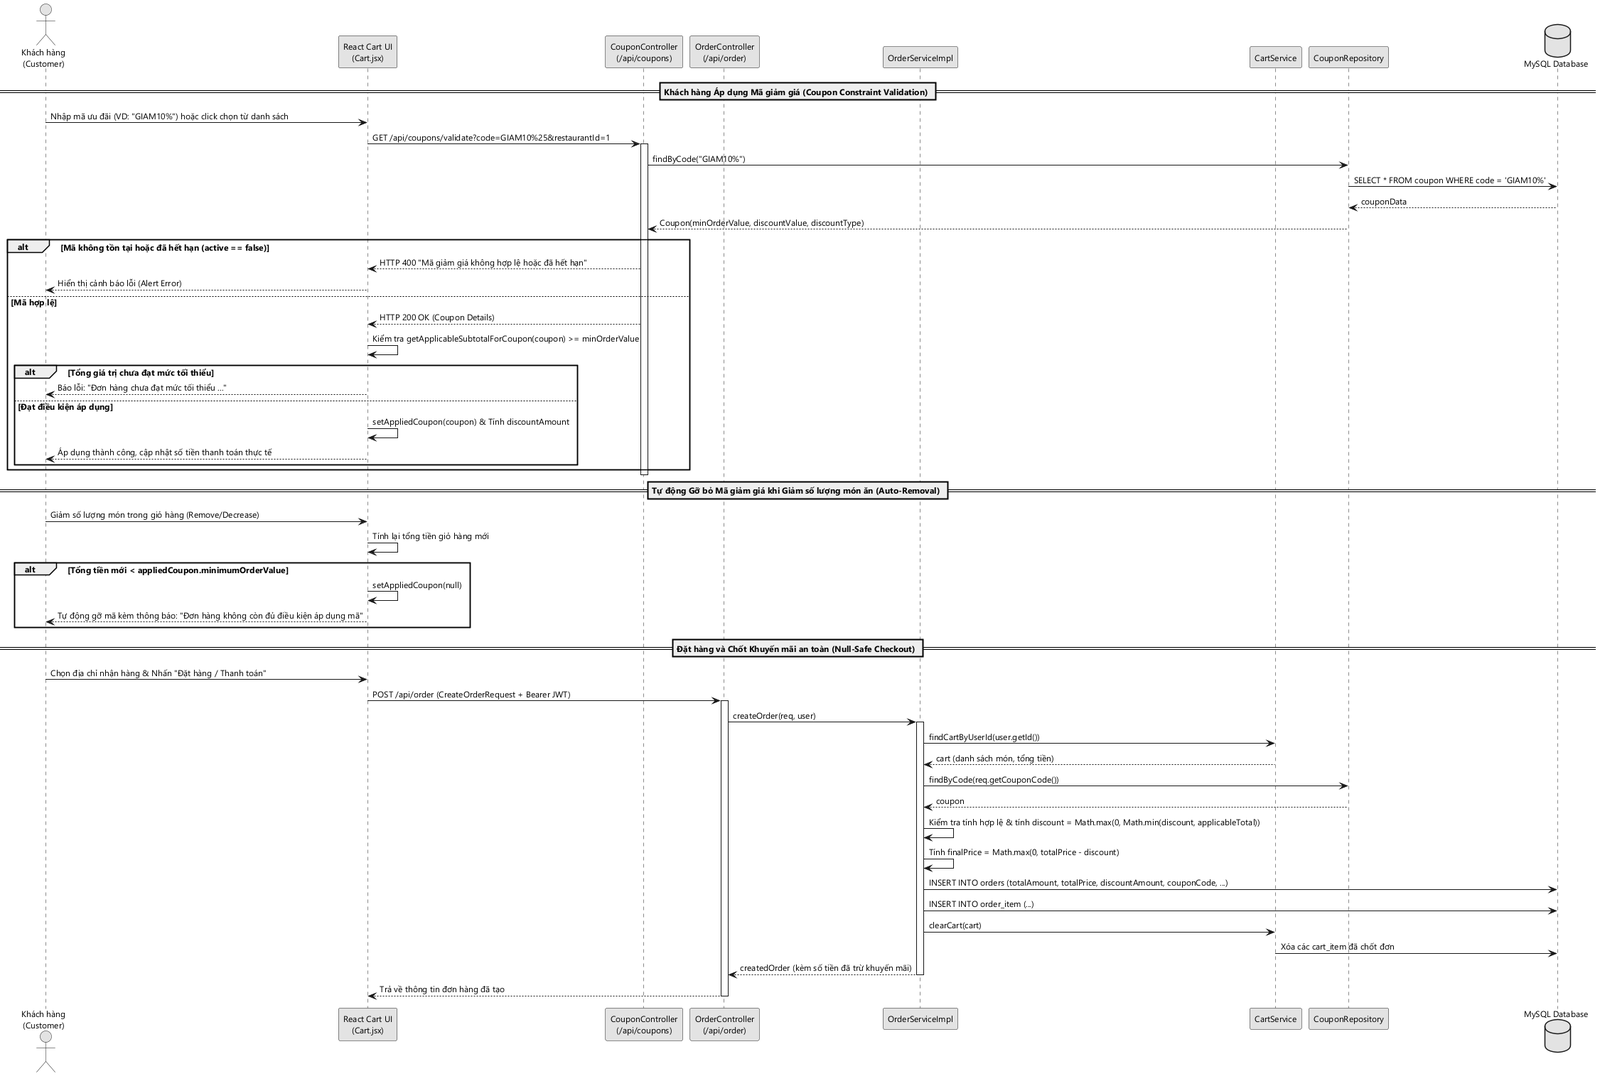
\includegraphics[width=0.92\textwidth]{figures/fig_sequence_order_coupon.png}
\end{figure}

Sơ đồ Hình 4.3 làm rõ sự phối hợp hai lớp giữa Client và Server trong việc quản trị mã ưu đãi:
\begin{itemize}
    \item Phía Client thực hiện thẩm định trước các điều kiện đơn tối thiểu và tích hợp tính năng tự động gỡ bỏ mã (Auto-removal) nếu người dùng giảm số lượng món ăn khiến tổng tiền rớt xuống dưới ngưỡng tối thiểu.
    \item Phía Server tại \texttt{OrderServiceImpl} một lần nữa kiểm tra độc lập tính hợp lệ của mã, phạm vi áp dụng (theo nhà hàng hay toàn sàn) và áp dụng công thức an toàn biên \texttt{Math.max(0, Math.min(discount, applicableTotal))} để đảm bảo đơn hàng không bao giờ bị âm tiền hoặc bị gian lận.
\end{itemize}

\subsection{Biểu đồ Tuần tự: Thanh toán Đa phương thức (Stripe Checkout \& COD)}
Luồng phân nhánh thanh toán đa phương thức an toàn được mô tả trong Hình 4.4:

\begin{figure}{Biểu đồ tuần tự ca sử dụng Thanh toán Đa phương thức (Stripe Checkout \& COD)}
\centering
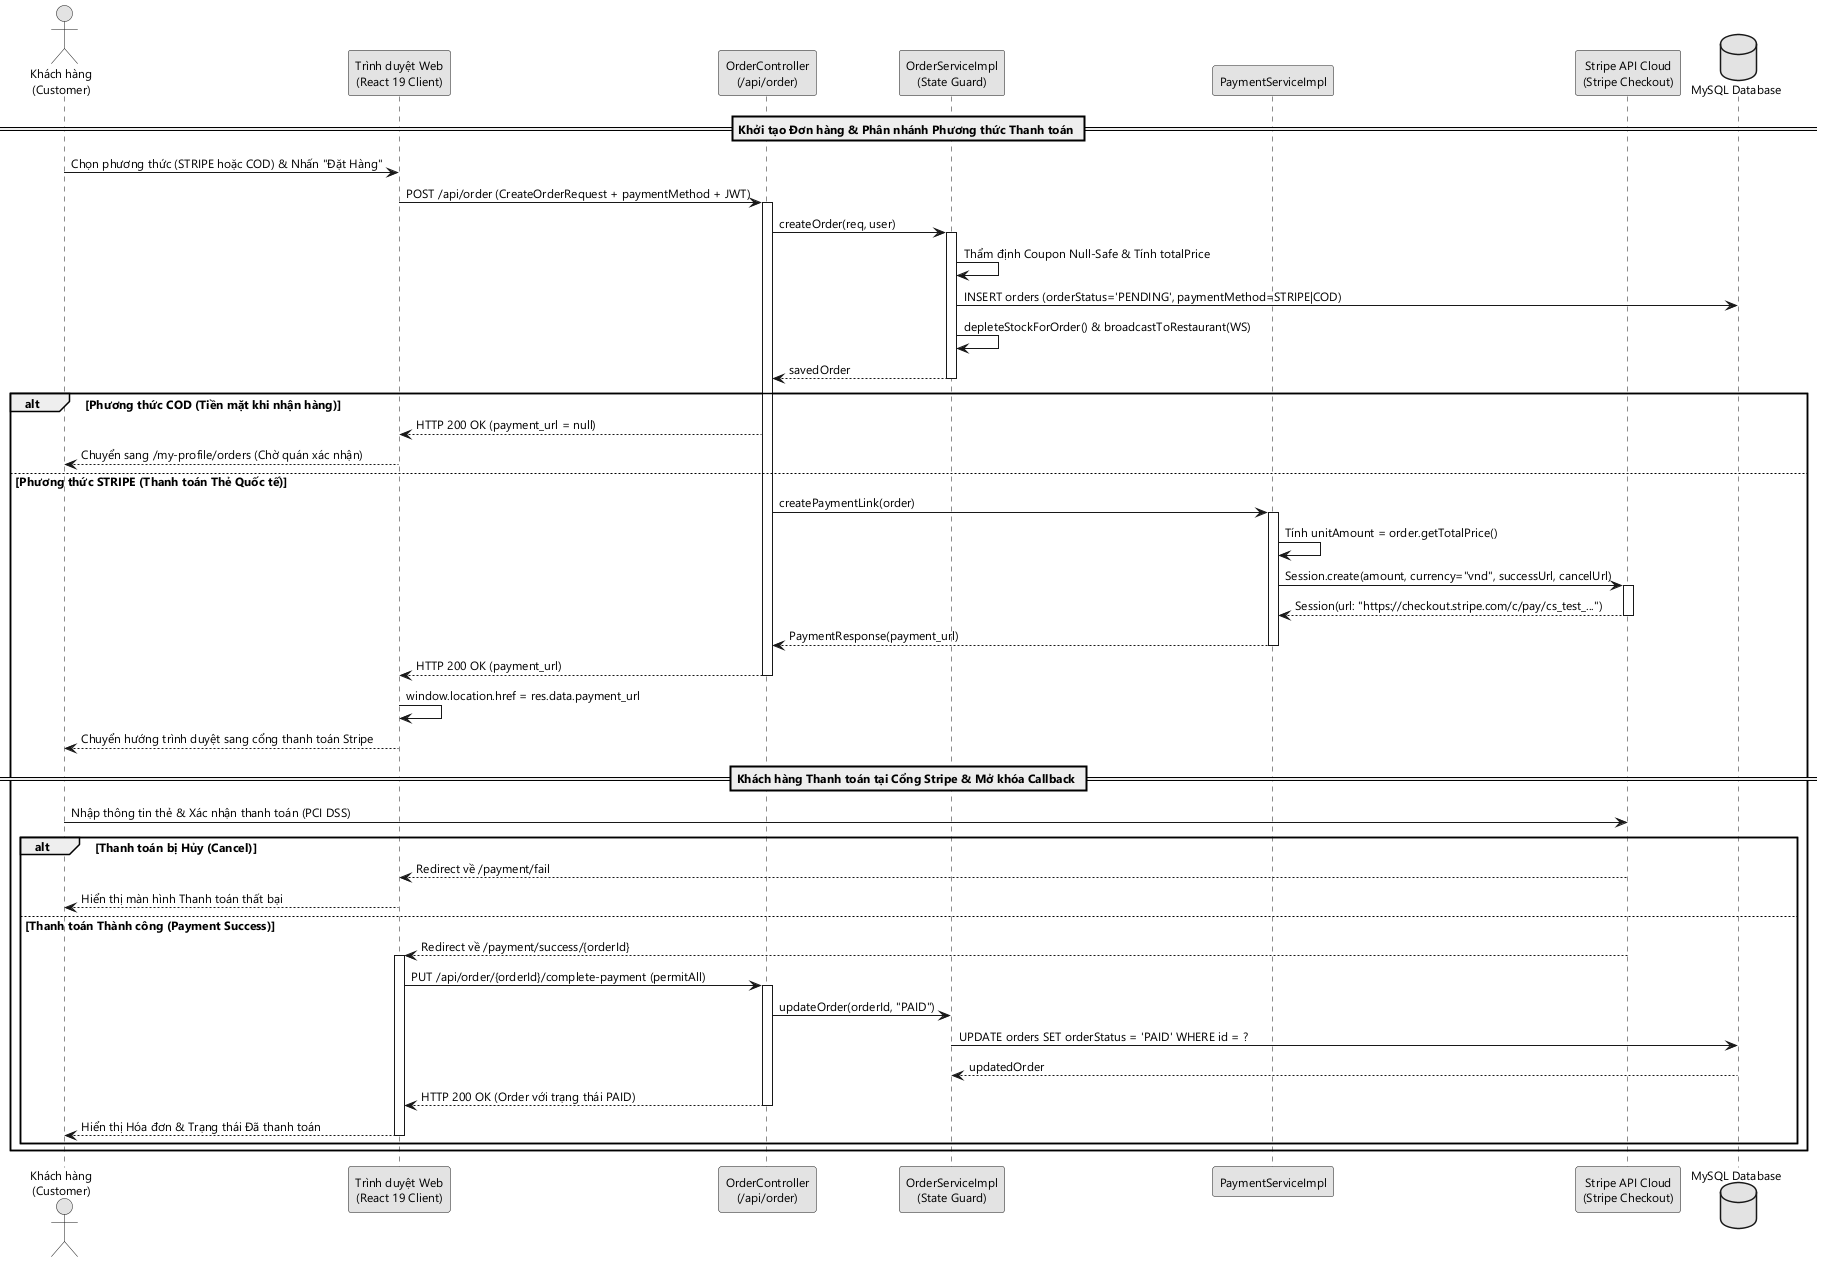
\includegraphics[width=0.92\textwidth]{figures/fig_sequence_stripe_payment.png}
\end{figure}

Hình 4.4 mô tả quá trình phân nhánh xử lý thông minh dựa trên \texttt{paymentMethod}: Nếu khách chọn \texttt{COD}, hệ thống lưu đơn hàng trạng thái \texttt{PENDING} và điều hướng ngay tới trang quản lý đơn (\texttt{payment\_url = null}). Nếu chọn \texttt{STRIPE}, máy chủ gọi Stripe SDK tạo Checkout Session theo số tiền sau giảm giá. Sau khi hoàn tất quẹt thẻ, trình duyệt chuyển về \texttt{/payment/success/:id} và gọi API callback \texttt{PUT /api/order/\{orderId\}/complete-payment} (đã được mở khóa \texttt{permitAll()} an toàn) để cập nhật dứt điểm trạng thái đơn hàng sang \texttt{PAID}.

\subsection{Biểu đồ Tuần tự: Tiếp nhận và Kiểm soát Máy trạng thái Đơn hàng}
Quy trình điều phối và bảo vệ trạng thái đơn hàng của chủ nhà hàng được thể hiện trong Hình 4.5:

\begin{figure}{Biểu đồ tuần tự ca sử dụng Tiếp nhận và Kiểm soát Máy trạng thái Đơn hàng}
\centering
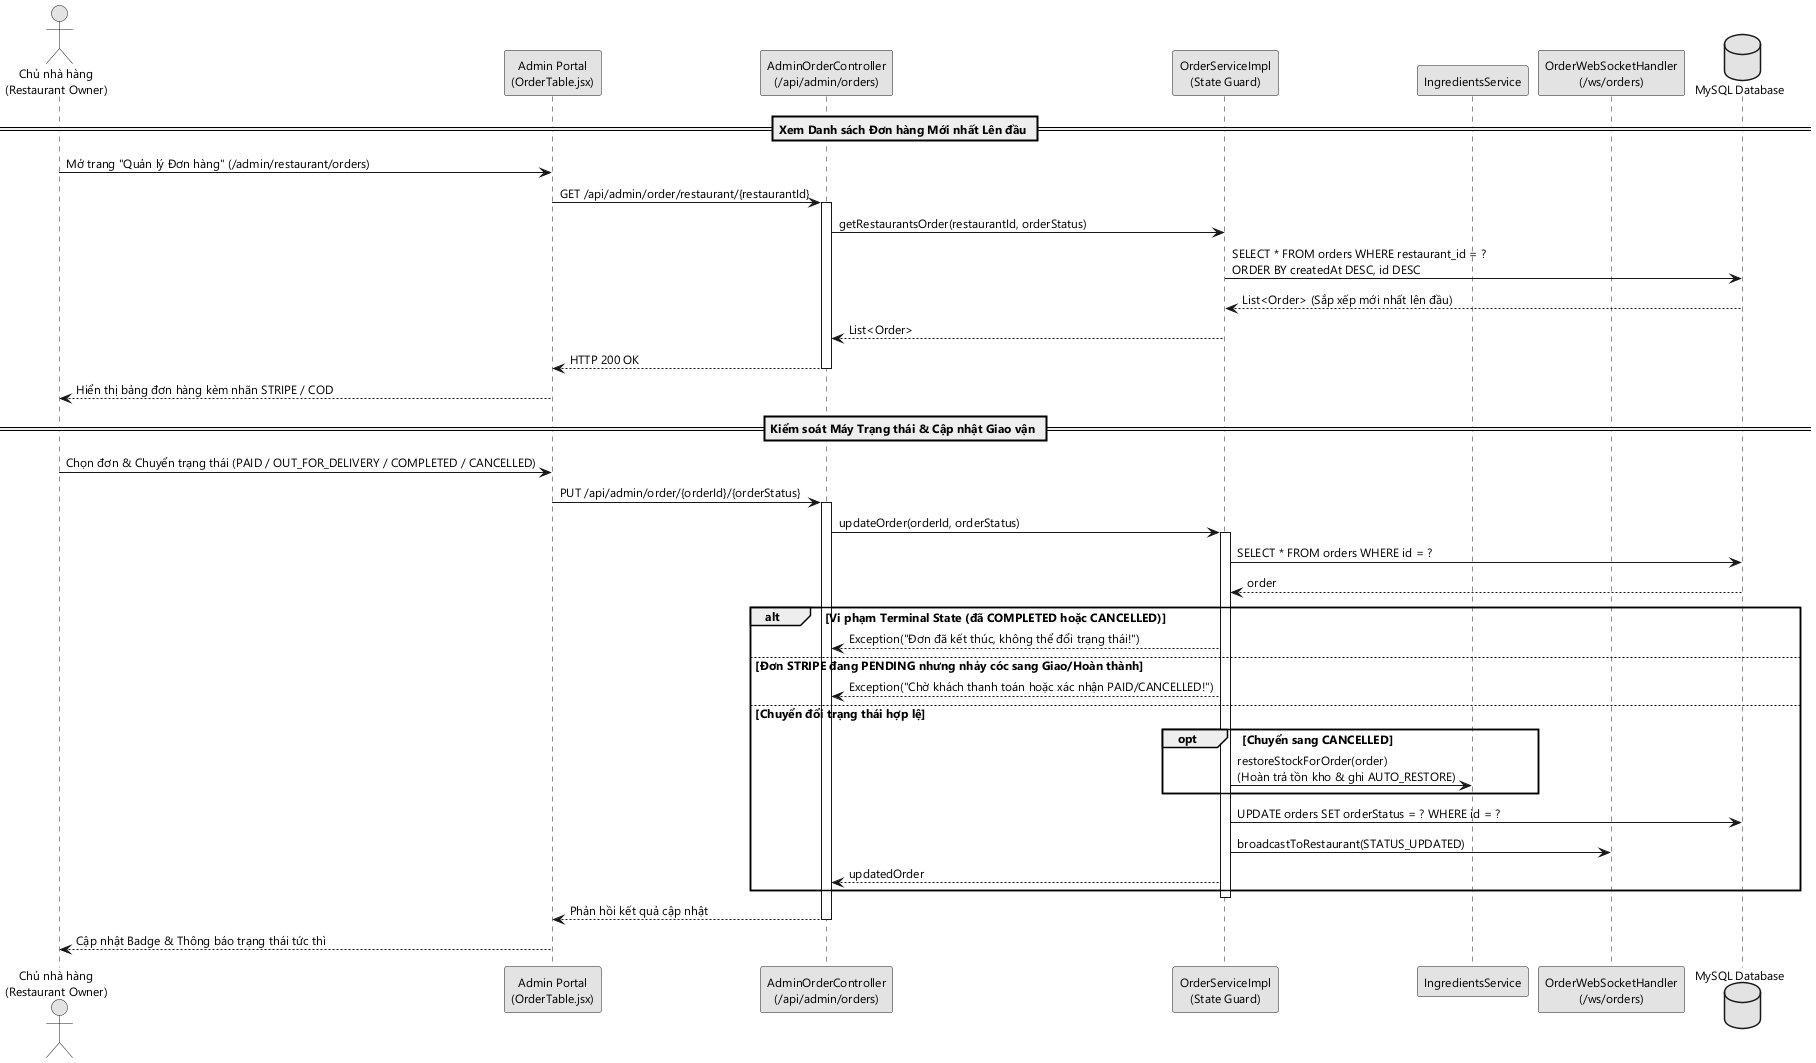
\includegraphics[width=0.92\textwidth]{figures/fig_sequence_order_status.png}
\end{figure}

Sơ đồ Hình 4.5 mô tả quy trình sắp xếp đơn hàng mới nhất lên đầu (\texttt{ORDER BY createdAt DESC, id DESC}) và bộ kiểm soát chuyển trạng thái (\textbf{Order State Guard}): hệ thống chặn mọi thao tác chỉnh sửa đối với đơn đã kết thúc (\texttt{COMPLETED}/\texttt{CANCELLED}), ngăn đơn Stripe \texttt{PENDING} nhảy cóc sang bước giao hàng nếu chưa xác nhận thanh toán, đồng thời tự động kích hoạt \texttt{restoreStockForOrder()} hoàn kho khi đơn bị hủy và phát sóng cập nhật qua WebSocket.

\subsection{Biểu đồ Tuần tự: Kiểm duyệt Đánh giá của Super Admin}
Quy trình bảo vệ môi trường văn hóa số trên sàn được thể hiện trong Hình 4.6:

\begin{figure}{Biểu đồ tuần tự ca sử dụng Kiểm duyệt đánh giá và nhà hàng vi phạm}
\centering
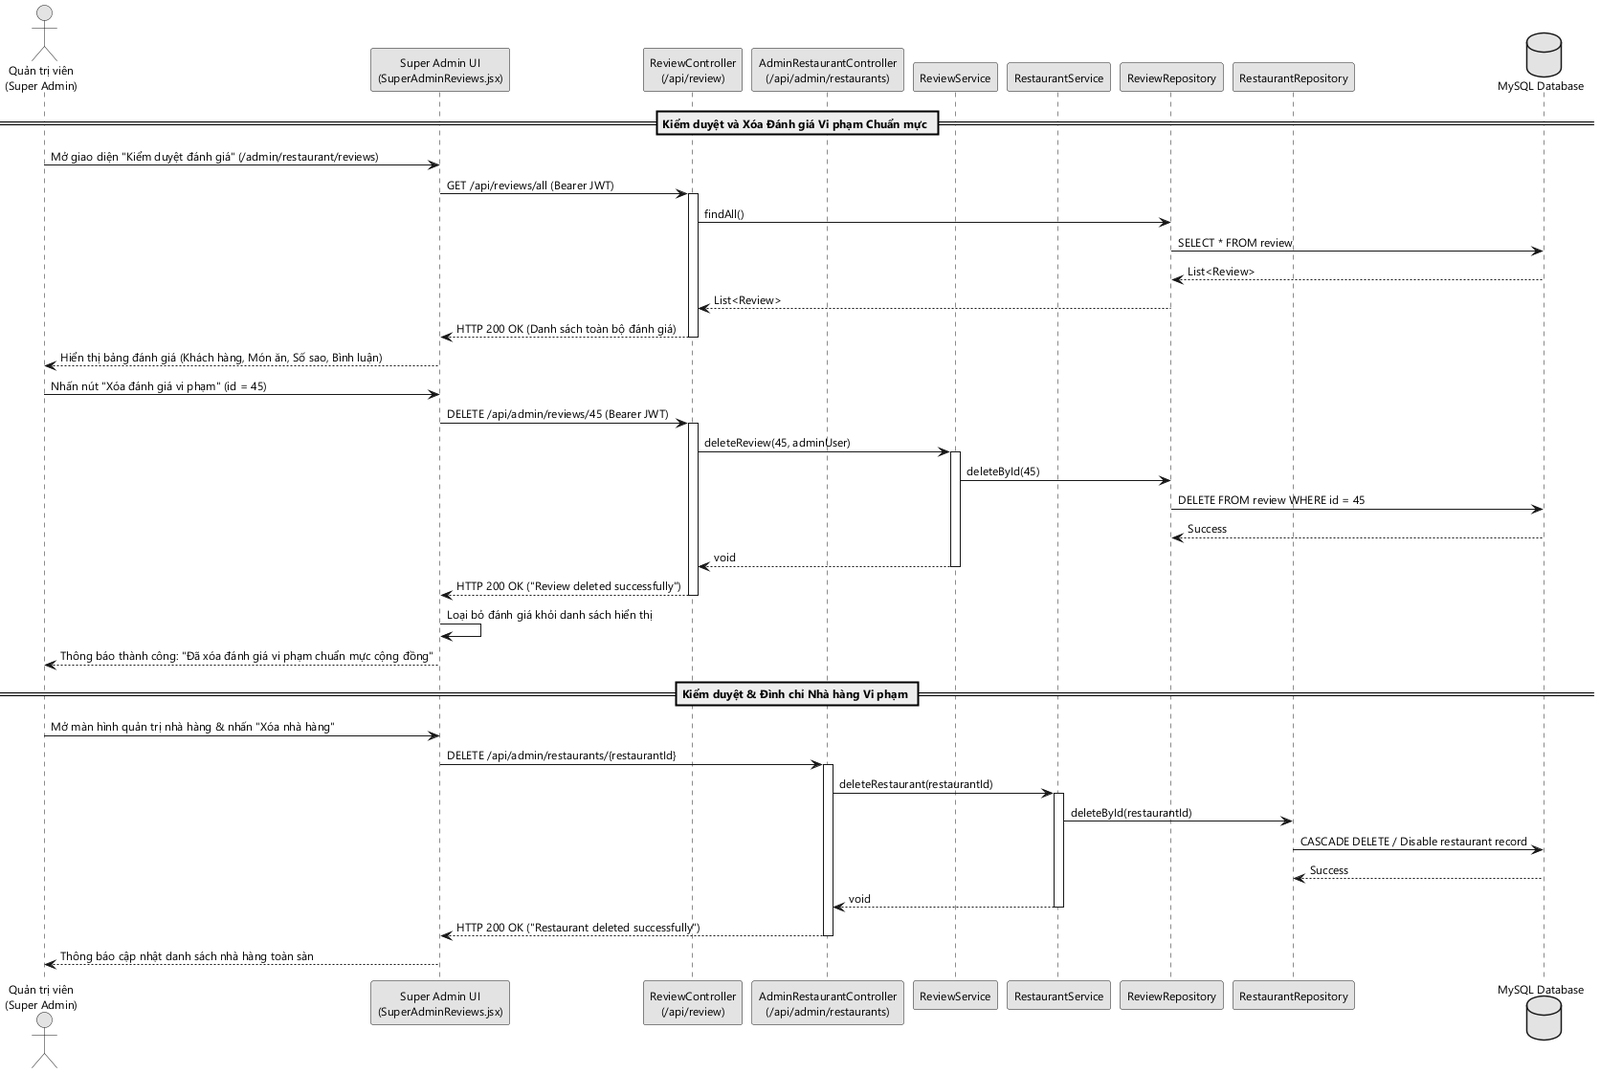
\includegraphics[width=0.92\textwidth]{figures/fig_sequence_admin_review.png}
\end{figure}

Hình 4.6 minh họa cách thức Quản trị viên tối cao rà soát các bài đánh giá theo từng nhà hàng và thực hiện quyền hạn gỡ bỏ bài viết độc hại hoặc đình chỉ các cơ sở nhà hàng có hành vi gian lận thông qua các API bảo vệ riêng biệt.

\subsection{Biểu đồ Tuần tự: Cảnh báo Đơn hàng WebSocket và Tác tử AI Copilot}
Quy trình truyền thông thời gian thực và điều phối Tác tử AI hành động được mô tả trong Hình 4.7:

\begin{figure}{Biểu đồ tuần tự Cảnh báo WebSocket và Tác tử AI Copilot Đa vai trò}
\centering
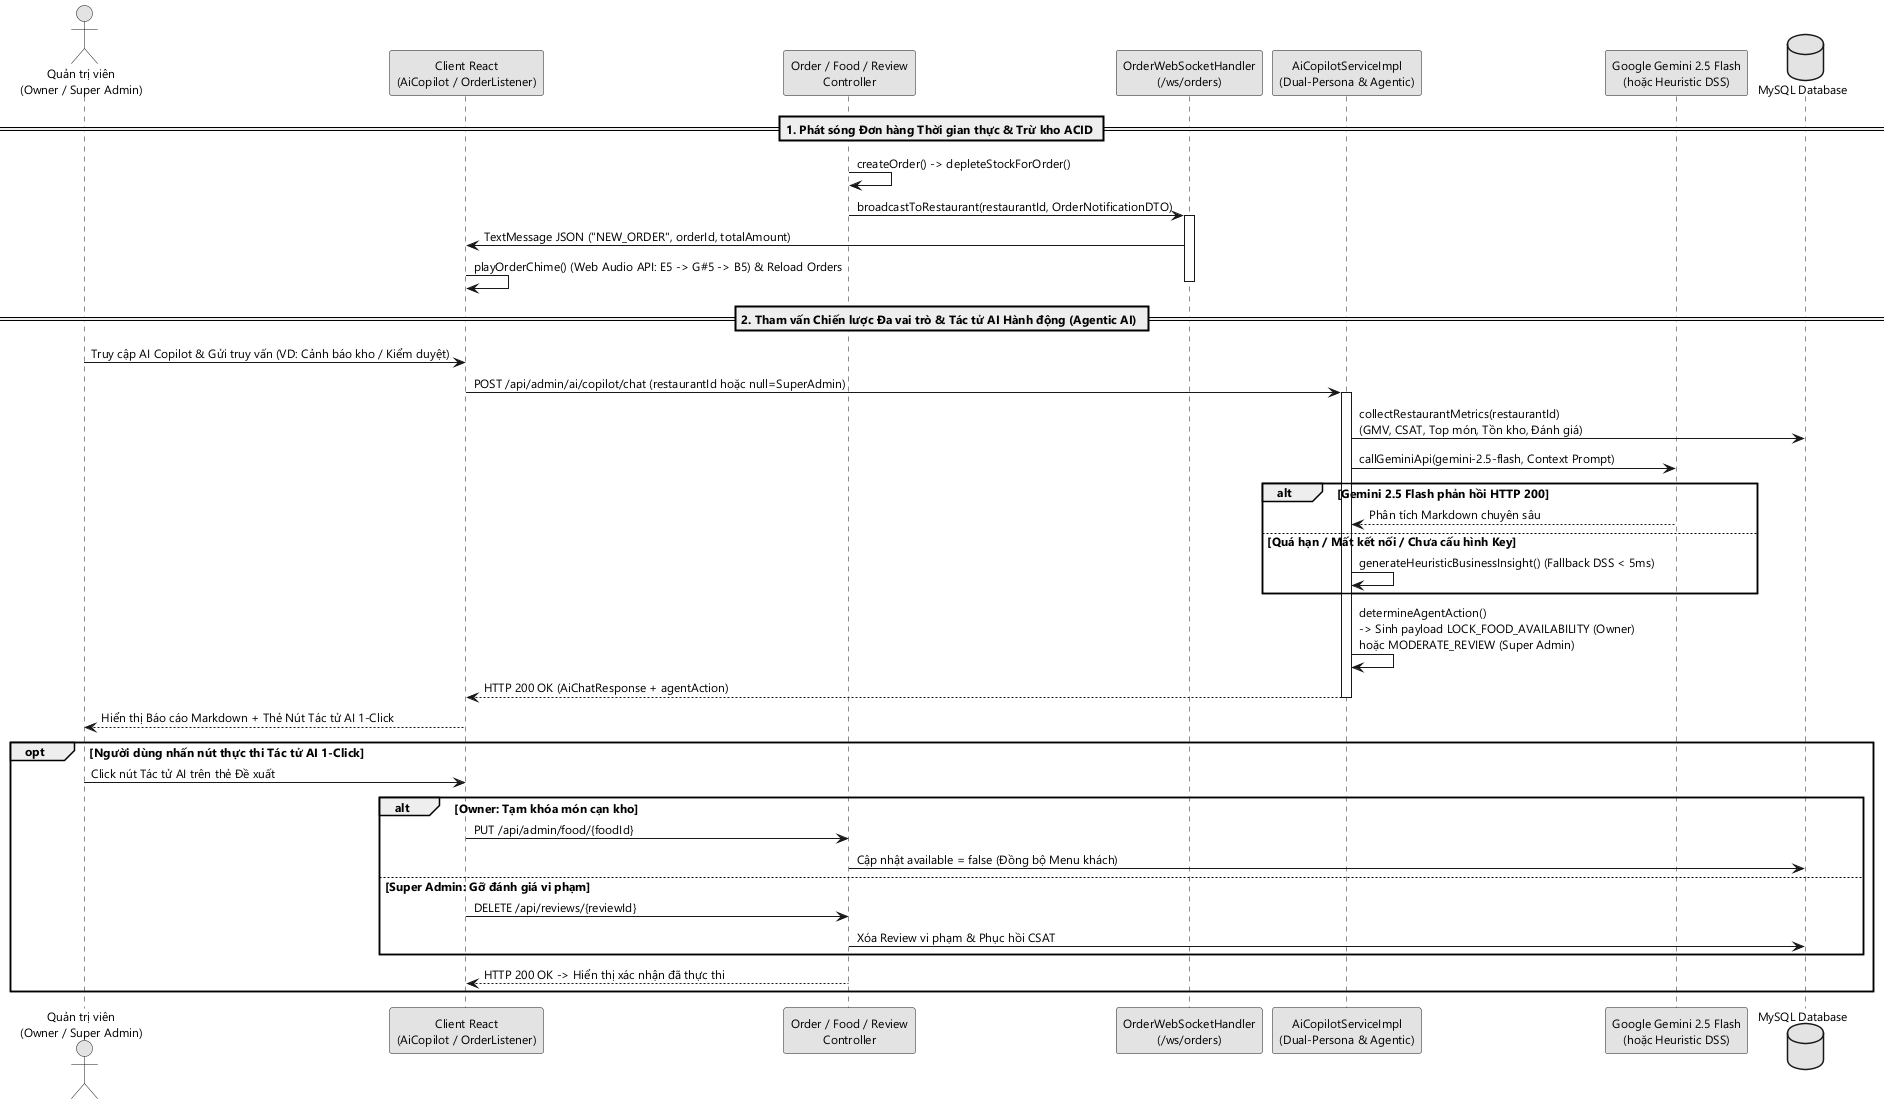
\includegraphics[width=0.92\textwidth]{figures/fig_sequence_websocket_ai.png}
\end{figure}

Sơ đồ Hình 4.7 minh họa sự phối hợp nhịp nhàng giữa hai luồng kỹ thuật nâng cao:
\begin{enumerate}
    \item \textbf{Luồng cảnh báo tức thời \& Trừ kho tự động:} Khi khách hàng tạo đơn hàng thành công tại \texttt{OrderServiceImpl}, hệ thống tự động kích hoạt dịch vụ kho \texttt{IngredientsServiceImpl.depleteStockForOrder} để khấu trừ định lượng nguyên liệu và ghi bản ghi biến động vào bảng \texttt{inventory\_log}. Ngay sau đó, đối tượng thông báo \texttt{OrderNotificationDTO} được đẩy tới \texttt{OrderWebSocketHandler.broadcastToRestaurant}. Tại trình duyệt của chủ nhà hàng, component \texttt{OrderNotificationListener.jsx} bắt sự kiện, gọi bộ tổng hợp âm thanh \texttt{playOrderChime()} tạo chuông ngân 3 nốt nhạc và cập nhật bảng đơn hàng tức thì mà không cần làm mới trang.
    \item \textbf{Luồng Tác tử AI Copilot Đa vai trò (Dual-Persona Agentic AI):} Khi Chủ quán (\texttt{restaurantId > 0}) hoặc Super Admin (\texttt{restaurantId = 0/null}) gửi truy vấn tại \texttt{AiCopilot.jsx}, dịch vụ \texttt{AiCopilotServiceImpl} thu thập chỉ số thực tế theo vai trò, gửi tới \textbf{Google Gemini 2.5 Flash} (hoặc tự động kích hoạt Động cơ Heuristic DSS dự phòng), đồng thời gọi \texttt{determineAgentAction()} để sinh kèm gói đề xuất hành động (\texttt{LOCK\_FOOD\_AVAILABILITY} hoặc \texttt{MODERATE\_REVIEW}). Chỉ với 1 thao tác bấm nút trên giao diện, Tác tử AI lập tức khóa món cạn kho hoặc gỡ bỏ đánh giá vi phạm xuống CSDL.
\end{enumerate}

\subsection{Biểu đồ Tuần tự: Tư vấn Ẩm thực Khách hàng AI Concierge (Menu Catalog RAG)}
Quy trình truy xuất thực đơn thực tế và điều hướng đặt món thông minh cho khách hàng được minh họa trong Hình 4.8:

\begin{figure}{Biểu đồ tuần tự Tư vấn Ẩm thực Khách hàng qua AI Concierge (Menu Catalog RAG)}
\centering
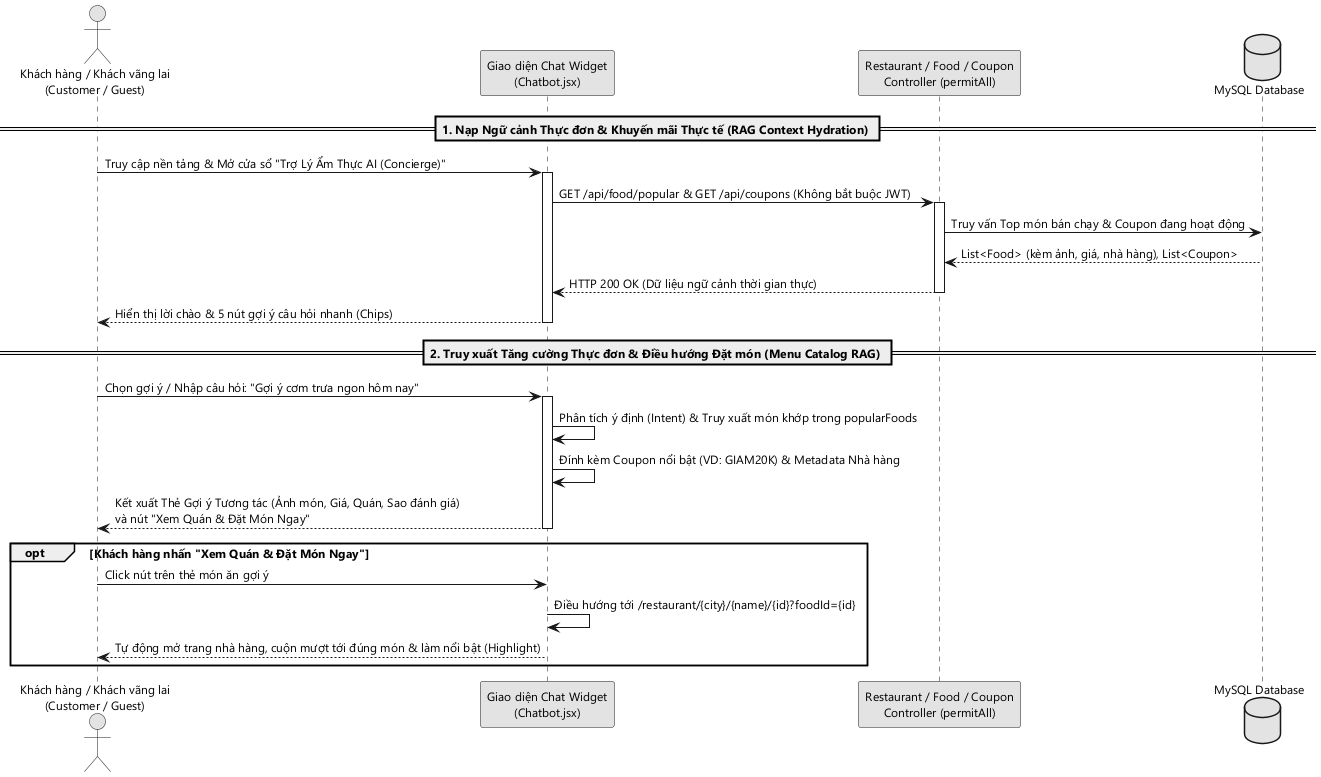
\includegraphics[width=0.92\textwidth]{figures/fig_sequence_chatbot_rag.png}
\end{figure}

Hình 4.8 làm rõ cơ chế RAG phía ứng dụng khách hàng: ngay khi khởi tạo, \texttt{Chatbot.jsx} nạp ngữ cảnh món bán chạy (\texttt{/api/food/popular}) và các mã khuyến mãi hoạt động (\texttt{/api/coupons}) thông qua các endpoint công khai (\texttt{permitAll}). Khi thực khách đặt câu hỏi hoặc nhấn gợi ý, thuật toán đối sánh ngữ cảnh sẽ ghép đúng món ăn kèm ảnh thật, giá bán và mã giảm giá vào một thẻ tương tác có gắn deep-link \texttt{?foodId=\{id\}} để khách hàng đi thẳng tới đúng món tại trang nhà hàng.

\section{Thiết kế Cơ sở Dữ liệu}
\subsection{Mô hình Thực thể Liên kết Hoàn chỉnh (ERD)}
Cơ sở dữ liệu của hệ thống được thiết kế theo chuẩn hóa dữ liệu quan hệ bậc ba (3NF) gồm 21 bảng/thực thể, đáp ứng toàn vẹn các mối quan hệ nghiệp vụ phức tạp của nền tảng ẩm thực. Sơ đồ thực thể liên kết được trình bày trong Hình 4.9:

\begin{figure}{Mô hình Thực thể Liên kết (ERD) Hoàn chỉnh 21 Bảng của Hệ thống}
\centering
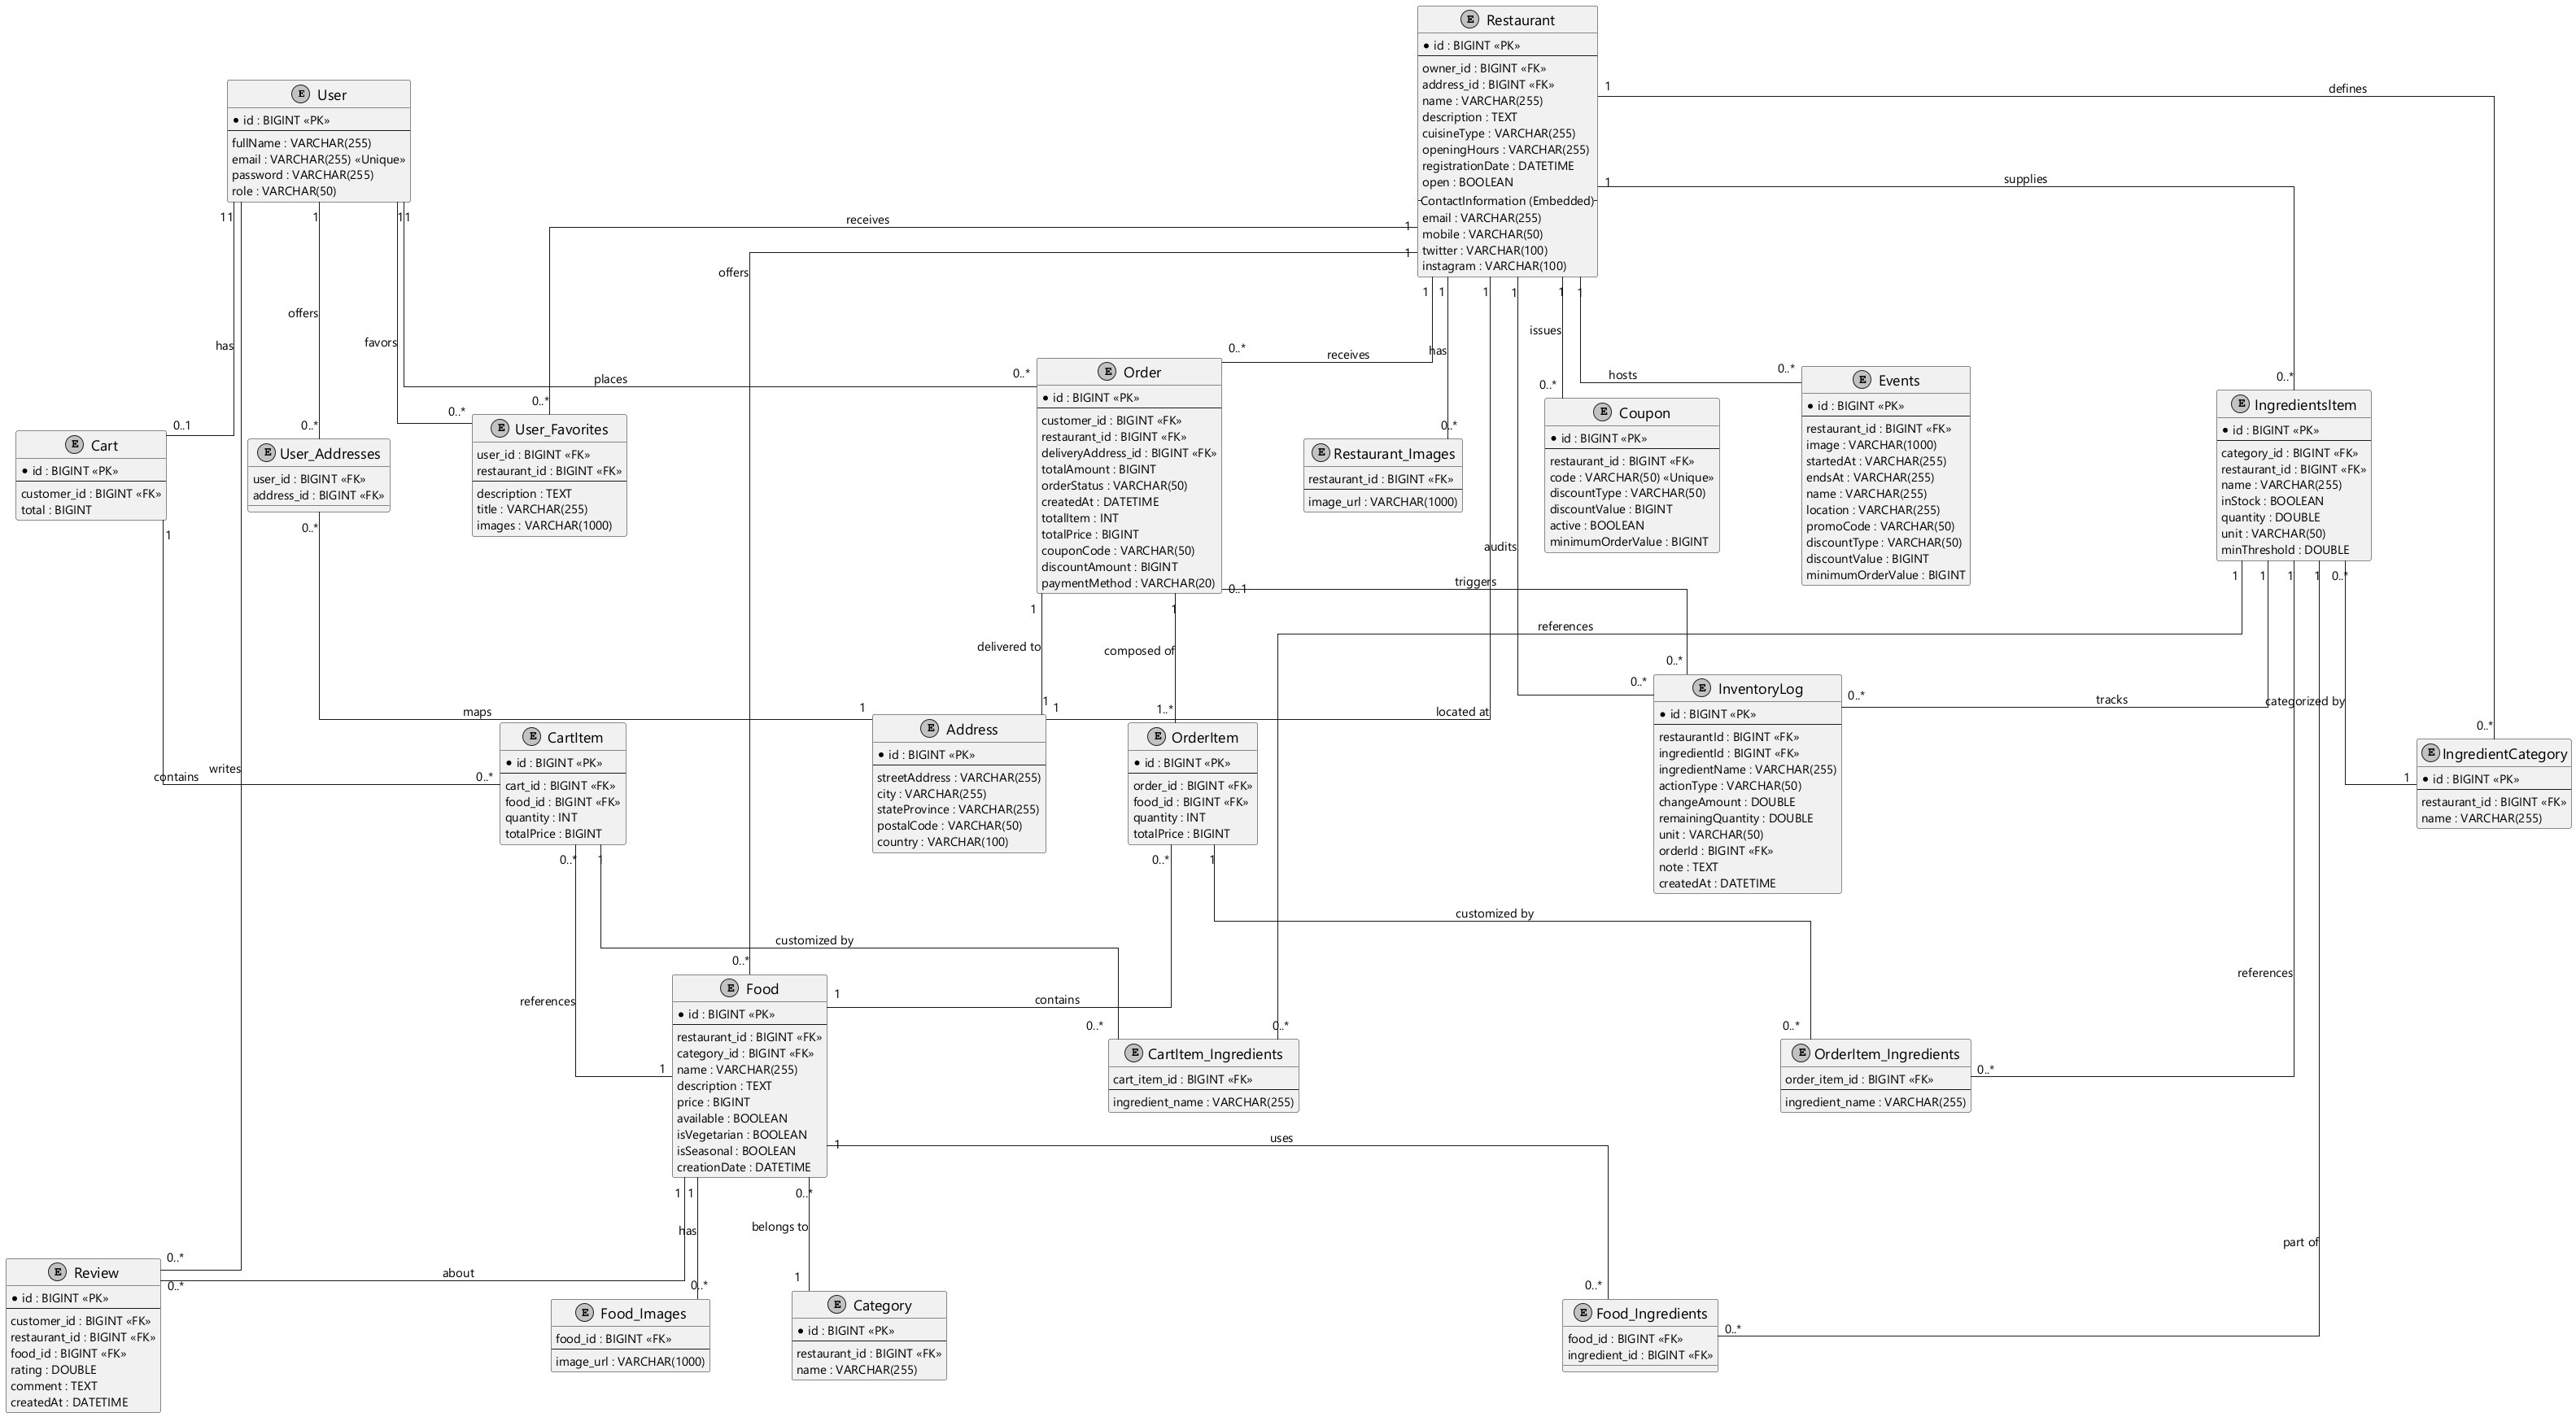
\includegraphics[width=0.96\textwidth]{figures/fig_erd_full.png}
\end{figure}

Mô hình dữ liệu trên bao quát đầy đủ các thực thể cốt lõi: người dùng (\texttt{User}), địa chỉ (\texttt{Address}), nhà hàng (\texttt{Restaurant}), thực đơn món ăn (\texttt{Food}), danh mục (\texttt{Category}), kho nguyên liệu phân nhóm (\texttt{IngredientCategory}, \texttt{IngredientsItem}), nhật ký xuất nhập tồn kho (\texttt{InventoryLog}), giỏ hàng (\texttt{Cart}, \texttt{CartItem}), đơn hàng (\texttt{Order}, \texttt{OrderItem}), mã ưu đãi (\texttt{Coupon}), sự kiện (\texttt{Events}) và đánh giá nhận xét (\texttt{Review}).

\subsection{Từ điển Dữ liệu Chi tiết (Data Dictionary)}
Dưới đây là từ điển dữ liệu đặc tả cấu trúc của các bảng trọng yếu nhất trong hệ thống:

% Bảng User
\begin{table}{Từ điển dữ liệu bảng User}
\centering
\small
\begin{tabular}{|l|l|l|l|}
\hline
\textbf{Tên trường} & \textbf{Kiểu dữ liệu} & \textbf{Ràng buộc} & \textbf{Mô tả ý nghĩa} \\ \hline
id & BIGINT & PK, Auto Increment & Khóa chính định danh người dùng \\ \hline
fullName & VARCHAR(255) & Not Null & Họ và tên đầy đủ của người dùng \\ \hline
email & VARCHAR(255) & Not Null, Unique & Email dùng để đăng nhập hệ thống \\ \hline
password & VARCHAR(255) & Not Null & Mật khẩu đã được mã hóa bằng BCrypt \\ \hline
role & VARCHAR(50) & Not Null & Vai trò người dùng (ROLE\_CUSTOMER, ...) \\ \hline
\end{tabular}
\end{table}

% Bảng Restaurant
\begin{table}{Từ điển dữ liệu bảng Restaurant}
\centering
\small
\begin{tabular}{|l|l|l|l|}
\hline
\textbf{Tên trường} & \textbf{Kiểu dữ liệu} & \textbf{Ràng buộc} & \textbf{Mô tả ý nghĩa} \\ \hline
id & BIGINT & PK, Auto Increment & Khóa chính định danh nhà hàng \\ \hline
owner\_id & BIGINT & FK (User.id) & Định danh chủ nhà hàng quản lý \\ \hline
address\_id & BIGINT & FK (Address.id) & Địa chỉ vật lý của nhà hàng \\ \hline
name & VARCHAR(255) & Not Null & Tên thương hiệu của nhà hàng \\ \hline
description & TEXT & Nullable & Mô tả phong cách ẩm thực của quán \\ \hline
cuisineType & VARCHAR(255) & Not Null & Thể loại ẩm thực (Phở, Pizza, Burger...) \\ \hline
openingHours & VARCHAR(255) & Nullable & Khung giờ mở cửa hoạt động hàng ngày \\ \hline
open & BOOLEAN & Default True & Cờ xác định nhà hàng có mở cửa nhận đơn \\ \hline
email & VARCHAR(255) & Nullable & Email liên hệ công khai của nhà hàng \\ \hline
mobile & VARCHAR(50) & Nullable & Số điện thoại hotline của nhà hàng \\ \hline
registrationDate & DATETIME & Not Null & Thời điểm đăng ký tham gia sàn \\ \hline
\end{tabular}
\end{table}

% Bảng Food
\begin{table}{Từ điển dữ liệu bảng Food}
\centering
\small
\begin{tabular}{|l|l|l|l|}
\hline
\textbf{Tên trường} & \textbf{Kiểu dữ liệu} & \textbf{Ràng buộc} & \textbf{Mô tả ý nghĩa} \\ \hline
id & BIGINT & PK, Auto Increment & Khóa chính định danh món ăn \\ \hline
restaurant\_id & BIGINT & FK (Restaurant.id) & Nhà hàng cung cấp món ăn này \\ \hline
category\_id & BIGINT & FK (Category.id) & Danh mục món ăn thuộc nhà hàng \\ \hline
name & VARCHAR(255) & Not Null & Tên gọi của món ăn \\ \hline
description & TEXT & Nullable & Mô tả thành phần hương vị món ăn \\ \hline
price & BIGINT & Not Null & Giá bán niêm yết (Đơn vị: VNĐ) \\ \hline
available & BOOLEAN & Default True & Trạng thái món ăn còn hàng hay đã hết \\ \hline
isVegetarian & BOOLEAN & Default False & Đánh dấu món ăn chay \\ \hline
isSeasonal & BOOLEAN & Default False & Món ăn phục vụ theo mùa \\ \hline
creationDate & DATETIME & Not Null & Thời điểm tạo món ăn trên hệ thống \\ \hline
\end{tabular}
\end{table}

% Bảng IngredientsItem
\begin{table}{Từ điển dữ liệu bảng IngredientsItem (Định lượng tồn kho)}
\centering
\small
\begin{tabular}{|l|l|l|l|}
\hline
\textbf{Tên trường} & \textbf{Kiểu dữ liệu} & \textbf{Ràng buộc} & \textbf{Mô tả ý nghĩa} \\ \hline
id & BIGINT & PK, Auto Increment & Khóa chính định danh nguyên liệu \\ \hline
restaurant\_id & BIGINT & FK (Restaurant.id) & Nhà hàng sở hữu nguyên liệu \\ \hline
category\_id & BIGINT & FK (IngredientCategory.id) & Nhóm danh mục nguyên liệu \\ \hline
name & VARCHAR(255) & Not Null & Tên nguyên liệu (Thêm phô mai, Bò viên...) \\ \hline
inStock & BOOLEAN & Default True & Cờ trạng thái nguyên liệu còn trong kho \\ \hline
quantity & DOUBLE & Default 0.0 & Số lượng tồn kho định lượng hiện tại \\ \hline
unit & VARCHAR(50) & Default 'phần' & Đơn vị đo lường (kg, gram, phần, lít) \\ \hline
minThreshold & DOUBLE & Default 5.0 & Ngưỡng định lượng cảnh báo sắp hết hàng \\ \hline
\end{tabular}
\end{table}

% Bảng InventoryLog
\begin{table}{Từ điển dữ liệu bảng InventoryLog (Nhật ký xuất nhập tồn kho)}
\centering
\small
\begin{tabular}{|l|l|l|l|}
\hline
\textbf{Tên trường} & \textbf{Kiểu dữ liệu} & \textbf{Ràng buộc} & \textbf{Mô tả ý nghĩa} \\ \hline
id & BIGINT & PK, Auto Increment & Khóa chính định danh bản ghi nhật ký kho \\ \hline
restaurantId & BIGINT & Not Null & Định danh nhà hàng phát sinh biến động kho \\ \hline
ingredientId & BIGINT & Not Null & Định danh nguyên liệu bị tác động \\ \hline
ingredientName & VARCHAR(255) & Not Null & Tên nguyên liệu tại thời điểm ghi nhận \\ \hline
actionType & VARCHAR(50) & Not Null & Loại hành động (AUTO\_DEPLETION, AUTO\_RESTORE, ...) \\ \hline
changeAmount & DOUBLE & Not Null & Lượng thay đổi (+ nhập thêm, - xuất món) \\ \hline
remainingQuantity & DOUBLE & Not Null & Số lượng tồn kho tức thời sau biến động \\ \hline
unit & VARCHAR(50) & Nullable & Đơn vị đo lường của nguyên liệu \\ \hline
orderId & BIGINT & Nullable & Mã đơn hàng liên quan (nếu do đơn kích hoạt) \\ \hline
note & TEXT & Nullable & Diễn giải chi tiết lý do biến động kho \\ \hline
createdAt & DATETIME & Not Null & Dấu thời gian ghi nhận biến động \\ \hline
\end{tabular}
\end{table}

% Bảng Cart & CartItem
\begin{table}{Từ điển dữ liệu bảng Cart và CartItem}
\centering
\small
\begin{tabular}{|l|l|l|l|}
\hline
\textbf{Tên trường} & \textbf{Kiểu dữ liệu} & \textbf{Ràng buộc} & \textbf{Mô tả ý nghĩa} \\ \hline
\multicolumn{4}{|c|}{\textbf{Bảng Cart}} \\ \hline
id & BIGINT & PK, Auto Increment & Khóa chính định danh giỏ hàng \\ \hline
customer\_id & BIGINT & FK (User.id) & Người dùng sở hữu giỏ hàng \\ \hline
total & BIGINT & Default 0 & Tổng tiền tạm tính của giỏ hàng \\ \hline
\multicolumn{4}{|c|}{\textbf{Bảng CartItem}} \\ \hline
id & BIGINT & PK, Auto Increment & Khóa chính định danh mục món trong giỏ \\ \hline
cart\_id & BIGINT & FK (Cart.id) & Giỏ hàng chứa mục món này \\ \hline
food\_id & BIGINT & FK (Food.id) & Món ăn được chọn \\ \hline
quantity & INT & Default 1 & Số lượng món ăn khách đặt \\ \hline
totalPrice & BIGINT & Not Null & Thành tiền = Giá món $\times$ Số lượng \\ \hline
\end{tabular}
\end{table}

% Bảng Order
\begin{table}{Từ điển dữ liệu bảng Order}
\centering
\small
\begin{tabular}{|l|l|l|l|}
\hline
\textbf{Tên trường} & \textbf{Kiểu dữ liệu} & \textbf{Ràng buộc} & \textbf{Mô tả ý nghĩa} \\ \hline
id & BIGINT & PK, Auto Increment & Khóa chính định danh đơn hàng \\ \hline
customer\_id & BIGINT & FK (User.id) & Khách hàng thực hiện đặt đơn \\ \hline
restaurant\_id & BIGINT & FK (Restaurant.id) & Nhà hàng tiếp nhận và chế biến đơn \\ \hline
deliveryAddress\_id & BIGINT & FK (Address.id) & Địa chỉ giao hàng đã lưu \\ \hline
totalAmount & BIGINT & Not Null & Tổng tiền đơn hàng trước khi trừ ưu đãi \\ \hline
discountAmount & BIGINT & Default 0 & Số tiền được chiết khấu từ mã ưu đãi \\ \hline
totalPrice & BIGINT & Not Null & Số tiền thanh toán thực tế cuối cùng \\ \hline
couponCode & VARCHAR(50) & Nullable & Mã giảm giá đã được áp dụng vào đơn \\ \hline
orderStatus & VARCHAR(50) & Not Null & Trạng thái: PENDING, PAID, OUT\_FOR\_DELIVERY... \\ \hline
paymentMethod & VARCHAR(20) & Default 'STRIPE' & Phương thức thanh toán: STRIPE hoặc COD \\ \hline
createdAt & DATETIME & Not Null & Thời điểm khởi tạo đơn hàng \\ \hline
totalItem & INT & Not Null & Tổng số lượng món ăn có trong đơn \\ \hline
\end{tabular}
\end{table}

% Bảng Events
\begin{table}{Từ điển dữ liệu bảng Events (Sự kiện đồng bộ Mã ưu đãi)}
\centering
\small
\begin{tabular}{|l|l|l|l|}
\hline
\textbf{Tên trường} & \textbf{Kiểu dữ liệu} & \textbf{Ràng buộc} & \textbf{Mô tả ý nghĩa} \\ \hline
id & BIGINT & PK, Auto Increment & Khóa chính định danh sự kiện nhà hàng \\ \hline
restaurant\_id & BIGINT & FK (Restaurant.id) & Nhà hàng tổ chức sự kiện khuyến mãi \\ \hline
name & VARCHAR(255) & Not Null & Tên chương trình sự kiện ẩm thực \\ \hline
location & VARCHAR(255) & Nullable & Địa điểm áp dụng sự kiện của quán \\ \hline
startedAt & VARCHAR(255) & Nullable & Thời điểm bắt đầu áp dụng ưu đãi \\ \hline
endsAt & VARCHAR(255) & Nullable & Thời điểm kết thúc chương trình \\ \hline
promoCode & VARCHAR(50) & Nullable & Mã ưu đãi gắn sự kiện (tự đồng bộ sang Coupon) \\ \hline
discountType & VARCHAR(50) & Default 'PERCENTAGE' & Loại giảm giá: PERCENTAGE hoặc FLAT \\ \hline
discountValue & BIGINT & Default 0 & Giá trị ưu đãi (\% hoặc VNĐ) \\ \hline
minimumOrderValue & BIGINT & Default 0 & Giá trị đơn tối thiểu được hưởng ưu đãi \\ \hline
\end{tabular}
\end{table}

% Bảng Coupon
\begin{table}{Từ điển dữ liệu bảng Coupon}
\centering
\small
\begin{tabular}{|l|l|l|l|}
\hline
\textbf{Tên trường} & \textbf{Kiểu dữ liệu} & \textbf{Ràng buộc} & \textbf{Mô tả ý nghĩa} \\ \hline
id & BIGINT & PK, Auto Increment & Khóa chính định danh mã giảm giá \\ \hline
restaurant\_id & BIGINT & FK (Restaurant.id), Null & Mã riêng của quán (nếu có) hoặc toàn sàn \\ \hline
code & VARCHAR(50) & Not Null, Unique & Ký tự mã ưu đãi (Ví dụ: GIAM10\%) \\ \hline
discountType & VARCHAR(50) & Not Null & Loại chiết khấu: PERCENTAGE hoặc FLAT \\ \hline
discountValue & BIGINT & Not Null & Giá trị chiết khấu (\% hoặc số tiền VNĐ) \\ \hline
minimumOrderValue & BIGINT & Default 0 & Ngưỡng tiền đơn hàng tối thiểu để áp dụng \\ \hline
active & BOOLEAN & Default True & Trạng thái mã còn hiệu lực sử dụng \\ \hline
\end{tabular}
\end{table}

% Bảng Review
\begin{table}{Từ điển dữ liệu bảng Review}
\centering
\small
\begin{tabular}{|l|l|l|l|}
\hline
\textbf{Tên trường} & \textbf{Kiểu dữ liệu} & \textbf{Ràng buộc} & \textbf{Mô tả ý nghĩa} \\ \hline
id & BIGINT & PK, Auto Increment & Khóa chính định danh bài đánh giá \\ \hline
customer\_id & BIGINT & FK (User.id) & Khách hàng gửi bài đánh giá \\ \hline
restaurant\_id & BIGINT & FK (Restaurant.id) & Nhà hàng nhận đánh giá \\ \hline
food\_id & BIGINT & FK (Food.id), Nullable & Món ăn cụ thể được nhận xét \\ \hline
rating & DOUBLE & Not Null & Điểm số đánh giá từ 1.0 đến 5.0 sao \\ \hline
comment & TEXT & Nullable & Nội dung bình luận, phản hồi thực tế \\ \hline
createdAt & DATETIME & Not Null & Thời điểm đăng bài đánh giá \\ \hline
\end{tabular}
\end{table}

% =========================================================================
% CHƯƠNG 5: XÂY DỰNG VÀ TRIỂN KHAI ỨNG DỤNG
% =========================================================================
\chapter{XÂY DỰNG VÀ TRIỂN KHAI ỨNG DỤNG}

\section{Môi trường Phát triển và Thư viện Sử dụng}
\subsection{Môi trường Phần cứng và Phần mềm}
Hệ thống được thiết kế, lập trình và kiểm thử toàn diện trên môi trường công nghệ tiêu chuẩn:
\begin{itemize}
    \item \textbf{Hệ điều hành:} Microsoft Windows 11 Pro 64-bit.
    \item \textbf{Môi trường thực thi Java:} Oracle OpenJDK 17 LTS / Java 23 SE Runtime Environment.
    \item \textbf{Công cụ phát triển (IDE):} Visual Studio Code, IntelliJ IDEA Ultimate, Antigravity IDE.
    \item \textbf{Môi trường Frontend:} Node.js v24.x, NPM v10.x, Vite v8.0.
    \item \textbf{Hệ quản trị CSDL:} MySQL Community Server 8.0 (cổng 3307) kết hợp MySQL Workbench.
    \item \textbf{Công cụ kiểm thử API:} Postman v11, Apache JMeter.
\end{itemize}

\subsection{Danh mục Công cụ và Thư viện Phần mềm Cốt lõi}
Bảng 5.1 tổng hợp các thư viện và khung ứng dụng chính phục vụ việc hiện thực hóa dự án:

\begin{table}{Danh mục các thư viện và công nghệ chính được sử dụng}
\centering
\small
\begin{tabular}{|l|l|l|}
\hline
\textbf{Tên Thư viện / Công cụ} & \textbf{Phân hệ} & \textbf{Chức năng kỹ thuật chính} \\ \hline
Spring Boot 3.4.0 & Backend & Khung ứng dụng chính, quản lý IoC/DI và máy chủ nhúng \\ \hline
Spring Security & Backend & Quản lý bảo mật, FilterChain phân quyền và hỗ trợ Guest Browsing \\ \hline
jjwt (Java JWT) 0.11.5 & Backend & Sinh, giải mã và xác thực chữ ký mã thông báo JWT \\ \hline
Spring Data JPA / Hibernate & Backend & Ánh xạ đối tượng quan hệ ORM và quản lý giao dịch CSDL \\ \hline
Spring WebSocket & Backend & Quản lý kênh truyền thông hai chiều thời gian thực và phát sóng sự kiện \\ \hline
Google Gemini 2.5 Flash API & Backend & Tích hợp mô hình ngôn ngữ lớn LLM hỗ trợ phân tích và điều hành \\ \hline
Stripe Java SDK 24.12.0 & Backend & Tích hợp cổng thanh toán trực tuyến Stripe Checkout Session \\ \hline
React 19.2.6 & Frontend & Thư viện lõi xây dựng giao diện người dùng theo Component \\ \hline
Redux Toolkit 2.12.0 (RTK) & Frontend & Quản lý trạng thái toàn cục ứng dụng một cách bất biến \\ \hline
React Router DOM 7.15.1 & Frontend & Quản lý định tuyến và điều hướng trang Single Page \\ \hline
Material-UI (MUI 9.0.1) & Frontend & Bộ thành phần giao diện người dùng chuyên nghiệp \\ \hline
TailwindCSS 3.4.19 & Frontend & Tiện ích xây dựng layout Responsive và màu sắc Dark Mode \\ \hline
Recharts 3.8.1 & Frontend & Kết xuất biểu đồ doanh thu và phân bổ đơn hàng trực quan \\ \hline
Web Audio API & Frontend & Tổng hợp chuông cảnh báo âm thanh thuật toán tương tác trực tiếp \\ \hline
Axios 1.16.1 & Frontend & Client HTTP gửi các yêu cầu API bất đồng bộ kèm Token \\ \hline
Formik 2.4 \& Yup 1.7 & Frontend & Quản lý form nhập liệu và kiểm tra tính hợp lệ dữ liệu Client \\ \hline
React Slick 0.31 & Frontend & Thư viện kết xuất thanh trượt tương tác Carousel món ăn \\ \hline
\end{tabular}
\end{table}

\section{Cài đặt các Chức năng Quan trọng của Hệ thống}
Phần này trình bày chi tiết mã nguồn hiện thực hóa các cơ chế cốt lõi trong hệ thống, bao gồm bảo mật phân quyền, động cơ khuyến mãi an toàn, dịch vụ thanh toán Stripe và quản lý trạng thái tập trung.

\subsection{Cài đặt Bảo mật Xác thực JWT và Chặn Leo thang Đặc quyền}
Tại tầng tiếp nhận đăng ký tài khoản \texttt{AuthController.java}, hệ thống áp dụng cơ chế kiểm duyệt nghiêm ngặt:

\begin{lstlisting}[language=Java, caption={Kiểm duyệt vai trò và tạo giỏ hàng tự động trong AuthController.java}]
@PostMapping("/signup")
public ResponseEntity<AuthResponse> createUserHandler(@RequestBody User user) throws Exception {
    User isEmailExist = userRepository.findByEmail(user.getEmail());
    if (isEmailExist != null) {
        throw new Exception("Email is already used with another account");
    }

    User createdUser = new User();
    createdUser.setEmail(user.getEmail());
    createdUser.setFullName(user.getFullName());
    
    // Ngan chan tuyet doi viec tu dang ky quyen Admin tu ben ngoai
    if (user.getRole() == USER_ROLE.ROLE_ADMIN) {
        throw new Exception("Registration as ADMIN is not allowed.");
    }
    createdUser.setRole(user.getRole() != null ? user.getRole() : USER_ROLE.ROLE_CUSTOMER);
    createdUser.setPassword(passwordEncoder.encode(user.getPassword()));

    User savedUser = userRepository.save(createdUser);

    // Tu dong tao gio hang trong ngay khi User dang ky thanh cong
    Cart cart = new Cart();
    cart.setCustomer(savedUser);
    cartRepository.save(cart);

    UserDetails userDetails = customUserDetailsService.loadUserByUsername(savedUser.getEmail());
    Authentication authentication = new UsernamePasswordAuthenticationToken(userDetails, null, userDetails.getAuthorities());
    SecurityContextHolder.getContext().setAuthentication(authentication);

    String jwt = jwtProvider.generateToken(authentication);

    AuthResponse authResponse = new AuthResponse();
    authResponse.setJwt(jwt);
    authResponse.setMessage("Register success");
    authResponse.setRole(savedUser.getRole());

    return new ResponseEntity<>(authResponse, HttpStatus.CREATED);
}
\end{lstlisting}

Đoạn mã trên thể hiện nguyên lý phòng thủ theo chiều sâu: ngay cả khi kẻ tấn công cố ý can thiệp vào Payload của HTTP POST request để gán \texttt{"role": "ROLE\_ADMIN"}, hệ thống sẽ phát hiện và ném ra ngoại lệ ngăn chặn, đảm bảo chỉ có tài khoản Super Admin duy nhất được sinh ra từ quy trình Auto-Seeding nội bộ mới có quyền quản trị tối cao.

Bên cạnh đó, để hỗ trợ khách vãng lai (Guest Browsing) tự do khám phá 16 nhà hàng, tìm kiếm món ăn, xem đánh giá và tương tác với Chatbot trước khi đăng nhập, bộ lọc bảo mật \texttt{AppConfig.java} mở quyền \texttt{permitAll()} cho các API đọc công khai và callback \texttt{PUT /api/order/*/complete-payment}, kết hợp cơ chế xử lý ngoại lệ nhẹ nhàng trong \texttt{JwtTokenValidator.java}:

\begin{lstlisting}[language=Java, caption={Cơ chế mở quyền Guest Browsing và dọn ngữ cảnh an toàn khi Token hết hạn}]
// Trong AppConfig.java: Mo quyen truy cap cong khai cho khach vang lai (Guest)
.requestMatchers(HttpMethod.GET, "/api/reviews/restaurant/**", "/api/reviews/food/**").permitAll()
.requestMatchers(HttpMethod.GET, "/api/coupons", "/api/food/popular", "/api/food/search").permitAll()
.requestMatchers(HttpMethod.GET, "/api/restaurants/**", "/api/category/restaurant/**", "/api/food/restaurant/**").permitAll()
.requestMatchers(HttpMethod.PUT, "/api/order/*/complete-payment").permitAll()

// Trong JwtTokenValidator.java: Neu JWT het han/loi, xoa SecurityContext de truy cap nhu Guest
} catch (Exception e) {
    SecurityContextHolder.clearContext();
}
\end{lstlisting}

\subsection{Cài đặt Động cơ Kiểm soát Khuyến mãi An toàn Biên (Null-Safe Coupon Engine)}
Tại tầng dịch vụ \texttt{OrderServiceImpl.java}, thuật toán xử lý mã giảm giá được xây dựng để kiểm soát mọi giá trị biên và ràng buộc ngưỡng tối thiểu:

\begin{lstlisting}[language=Java, caption={Thuật toán thẩm định và khấu trừ mã giảm giá an toàn trong OrderServiceImpl.java}]
// Ap dung Coupon giam gia neu co gui kem trong yeu cau dat hang
if (orderReq.getCouponCode() != null && !orderReq.getCouponCode().trim().isEmpty()) {
    Optional<Coupon> couponOpt = couponRepository.findByCodeAndRestaurantId(orderReq.getCouponCode(), restaurant.getId());
    if (!couponOpt.isPresent()) {
        // Kiem tra ma toan san neu khong phai ma rieng cua quan
        Optional<Coupon> globalCouponOpt = couponRepository.findByCode(orderReq.getCouponCode());
        if (globalCouponOpt.isPresent()) {
            couponOpt = globalCouponOpt;
        }
    }
    if (couponOpt.isPresent()) {
        Coupon coupon = couponOpt.get();
        if (coupon.isActive()) {
            long minOrderVal = coupon.getMinimumOrderValue() != null ? coupon.getMinimumOrderValue() : 0L;
            long applicableTotal = 0L;

            if (coupon.getRestaurant() != null) {
                // Ma rieng cua nha hang: Chi tinh tong tien cac mon thuoc quan do
                Long couponRestId = coupon.getRestaurant().getId();
                for (OrderItem oi : orderItems) {
                    if (oi.getFood() != null && oi.getFood().getRestaurant() != null 
                        && couponRestId.equals(oi.getFood().getRestaurant().getId())) {
                        applicableTotal += oi.getTotalPrice();
                    }
                }
                if (applicableTotal == 0) {
                    throw new Exception("Ma giam gia nay chi ap dung cho cac mon an cua nha hang " + coupon.getRestaurant().getName());
                }
                if (applicableTotal < minOrderVal) {
                    throw new Exception("Tong tien cac mon cua nha hang chua dat gia tri toi thieu " + minOrderVal + " d de ap dung.");
                }
            } else {
                // Ma toan san: Ap dung tren toan bo gia tri gio hang
                applicableTotal = totalPrice;
                if (applicableTotal < minOrderVal) {
                    throw new Exception("Don hang chua dat gia tri toi thieu " + minOrderVal + " d de ap dung ma giam gia nay.");
                }
            }

            long discount = 0;
            long discVal = coupon.getDiscountValue() != null ? coupon.getDiscountValue() : 0L;
            String discType = coupon.getDiscountType() != null ? coupon.getDiscountType() : "";
            if ("PERCENTAGE".equalsIgnoreCase(discType)) {
                discount = (applicableTotal * discVal) / 100;
            } else if ("FLAT".equalsIgnoreCase(discType)) {
                discount = discVal;
            }
            // Dam bao so tien giam khong am va khong vuot qua tong tien mon ap dung
            discount = Math.max(0, Math.min(discount, applicableTotal));
            createdOrder.setCouponCode(coupon.getCode());
            createdOrder.setDiscountAmount(discount);
            totalPrice = Math.max(0, totalPrice - discount);
        }
    }
}
\end{lstlisting}

Đoạn mã trên thể hiện tính chặt chẽ trong xử lý nghiệp vụ:
\begin{enumerate}
    \item Phân biệt rõ ràng giữa mã ưu đãi của riêng nhà hàng (chỉ tính tổng tiền trên các món của nhà hàng đó) và mã toàn sàn (áp dụng trên toàn bộ giỏ).
    \item Kiểm tra nghiêm ngặt ngưỡng tối thiểu \texttt{minOrderVal}.
    \item Dòng 46 sử dụng hàm toán học \texttt{Math.max(0, Math.min(discount, applicableTotal))} nhằm đảm bảo số tiền giảm giá không bao giờ bị âm và không bao giờ vượt quá tổng giá trị món ăn được hưởng ưu đãi.
    \item Dòng 49 đảm bảo số tiền thanh toán cuối cùng không bao giờ âm (\texttt{Math.max(0, totalPrice - discount)}).
\end{enumerate}

\subsection{Cài đặt Thanh toán Đa phương thức (Stripe Checkout \& COD) và Máy trạng thái Đơn hàng}
Hệ thống hỗ trợ linh hoạt hai phương thức thanh toán: qua cổng thẻ quốc tế Stripe hoặc tiền mặt khi nhận hàng (COD) tại \texttt{OrderController.java} và \texttt{PaymentServiceImpl.java}:

\begin{lstlisting}[language=Java, caption={Phân nhánh phương thức thanh toán và mở khóa Callback trong OrderController.java}]
@PostMapping("/order")
public ResponseEntity<PaymentResponse> createOrder(
        @RequestBody CreateOrderRequest req,
        @RequestHeader("Authorization") String jwt) throws Exception {
    User user = userService.findUserByJwtToken(jwt);
    Order order = orderService.createOrder(req, user);

    PaymentResponse res = new PaymentResponse();
    if (req.getPaymentMethod() != null && "COD".equalsIgnoreCase(req.getPaymentMethod().trim())) {
        res.setPayment_url(null);
    } else {
        // Mac dinh hoac chon thanh toan truc tuyen: goi Stripe Checkout Session
        res = paymentService.createPaymentLink(order);
    }
    return new ResponseEntity<>(res, HttpStatus.OK);
}

@PutMapping("/order/{orderId}/complete-payment")
public ResponseEntity<?> completePayment(@PathVariable Long orderId,
        @RequestHeader(value = "Authorization", required = false) String jwt) {
    try {
        Order updatedOrder = orderService.updateOrder(orderId, "PAID");
        return new ResponseEntity<>(updatedOrder, HttpStatus.OK);
    } catch (Exception e) {
        return new ResponseEntity<>(e.getMessage(), HttpStatus.INTERNAL_SERVER_ERROR);
    }
}
\end{lstlisting}

Song song đó, để ngăn ngừa lỗi vận hành bếp, lớp \texttt{OrderServiceImpl.java} cài đặt \textbf{Máy trạng thái Đơn hàng (Order State Guard)}: chặn thay đổi đối với các đơn đã ở trạng thái kết thúc (\texttt{COMPLETED}, \texttt{CANCELLED}), cấm đơn \texttt{STRIPE} đang chờ (\texttt{PENDING}) nhảy cóc sang bước giao hàng khi chưa thanh toán, tự động hoàn trả kho nguyên liệu (\texttt{restoreStockForOrder}) nếu chủ quán chuyển trạng thái sang hủy đơn, và truy vấn đơn hàng sắp xếp mới nhất lên đầu (\texttt{ORDER BY o.createdAt DESC, o.id DESC}) trong \texttt{OrderRepository.java}.

\subsection{Cài đặt Cơ chế Tự động Gỡ bỏ Mã Giảm giá ở Phía Client (Auto-Removal)}
Trong tệp giao diện giỏ hàng \texttt{Cart.jsx}, thuật toán theo dõi giá trị giỏ hàng được cài đặt thông qua React Hook \texttt{useEffect}:

\begin{lstlisting}[language=JavaScript, caption={Cơ chế Auto-Removal và URL Encoding mã ưu đãi trong Cart.jsx}]
// Tu dong kiem tra va go bo ma giam gia neu gio hang khong con du dieu kien
useEffect(() => {
    if (appliedCoupon && cartItems.length > 0) {
        const applicableSubtotal = getApplicableSubtotalForCoupon(appliedCoupon);
        const minOrderValue = appliedCoupon.minimumOrderValue || 0;
        
        if (applicableSubtotal < minOrderValue) {
            setAppliedCoupon(null);
            setPromoError(
                `Ma ${appliedCoupon.code} da tu dong go bo do don hang chua dat toi thieu ${minOrderValue.toLocaleString()} d`
            );
        }
    } else if (cartItems.length === 0 && appliedCoupon) {
        setAppliedCoupon(null);
    }
}, [cartTotal, cartItems]);

// Ap dung ma giam gia an toan ky tu dac biet
const applyCouponByCode = async (codeToApply, restId = null) => {
    if (!codeToApply || cartItems.length === 0) return;
    try {
        const targetRestId = restId || restaurantIds[0];
        // Ma hoa URI de bao ve ky tu dac biet nhu % khoi bi chan boi Firewall
        const safeCode = encodeURIComponent(codeToApply.trim().toUpperCase());
        const { data } = await api.get(
            `/api/coupons/validate?code=${safeCode}&restaurantId=${targetRestId}`, 
            { headers: { Authorization: `Bearer ${jwt}` } }
        );
        setAppliedCoupon(data);
        setPromoError("");
    } catch (err) {
        setPromoError(err.response?.data?.message || "Ma khuyen mai khong hop le");
    }
};
\end{lstlisting}

Nhờ đoạn mã trên, trải nghiệm người dùng luôn đảm bảo tính nhất quán: Khi người dùng giảm bớt số lượng món ăn khiến tổng tiền rớt xuống dưới mức tối thiểu quy định của voucher, giao diện ngay lập tức hủy trạng thái áp dụng mã kèm thông báo giải thích rõ ràng, tránh hoàn toàn tình huống xung đột khi gửi đơn lên máy chủ. Đồng thời, kỹ thuật \texttt{encodeURIComponent} tại dòng 24 bảo vệ an toàn cho các mã giảm giá có ký tự phần trăm (như \texttt{GIAM10\%}).

\subsection{Cài đặt Kênh WebSocket Phát sóng Đơn hàng Thời gian thực và Chuông Thuật toán}
Nhằm triệt tiêu độ trễ tiếp nhận đơn hàng, hệ thống xây dựng kênh truyền thông thời gian thực bằng Spring WebSocket kết hợp bộ tổng hợp âm thanh tương tác tại Client.

Tại tầng Backend, lớp \texttt{OrderWebSocketHandler.java} quản lý các phiên kết nối đồng thời và thực hiện phát sóng sự kiện:

\begin{lstlisting}[language=Java, caption={Quản lý phiên và phát sóng đơn hàng mới trong OrderWebSocketHandler.java}]
@Component
public class OrderWebSocketHandler extends TextWebSocketHandler {
    private final ObjectMapper objectMapper = new ObjectMapper();
    // Anh xa: restaurantId -> Set cac phien WebSocket dang ket noi
    private final Map<Long, Set<WebSocketSession>> restaurantSessions = new ConcurrentHashMap<>();
    private final Map<String, Long> sessionRestaurantMap = new ConcurrentHashMap<>();

    @Override
    protected void handleTextMessage(WebSocketSession session, TextMessage message) throws Exception {
        JsonNode root = objectMapper.readTree(message.getPayload());
        String type = root.has("type") ? root.get("type").asText() : "";
        if ("SUBSCRIBE_RESTAURANT".equalsIgnoreCase(type) && root.has("restaurantId")) {
            Long restaurantId = root.get("restaurantId").asLong();
            restaurantSessions.computeIfAbsent(restaurantId, k -> ConcurrentHashMap.newKeySet()).add(session);
            sessionRestaurantMap.put(session.getId(), restaurantId);
            // Gui xac nhan ket noi (ACK) ve phia Client
            session.sendMessage(new TextMessage("{\"type\":\"SUBSCRIBE_ACK\",\"status\":\"CONNECTED\"}"));
        }
    }

    public void broadcastToRestaurant(Long restaurantId, OrderNotificationDTO notification) {
        if (restaurantId == null || notification == null) return;
        Set<WebSocketSession> sessions = restaurantSessions.get(restaurantId);
        if (sessions == null || sessions.isEmpty()) return;

        try {
            String jsonPayload = objectMapper.writeValueAsString(notification);
            TextMessage textMessage = new TextMessage(jsonPayload);
            for (WebSocketSession s : sessions) {
                if (s.isOpen()) {
                    s.sendMessage(textMessage);
                }
            }
        } catch (Exception e) {
            System.err.println("[WebSocket] Error broadcasting alert: " + e.getMessage());
        }
    }
}
\end{lstlisting}

Phía Client tại tệp \texttt{soundAlert.js}, thay vì tải tệp âm thanh MP3 nặng nề và dễ bị trình duyệt chặn, ứng dụng sử dụng chuẩn Web Audio API để tổng hợp trực tiếp chuông 3 nốt nhạc hài hòa:

\begin{lstlisting}[language=JavaScript, caption={Tổng hợp chuông cảnh báo 3 âm sắc bằng Web Audio API trong soundAlert.js}]
export const playOrderChime = () => {
    try {
        const AudioContextClass = window.AudioContext || window.webkitAudioContext;
        if (!AudioContextClass) return;
        const ctx = new AudioContextClass();
        if (ctx.state === 'suspended') ctx.resume();

        // Chuoi am thanh chuong 3 not nhac: E5 -> G#5 -> B5 (Hop am truong vui tuoi)
        const notes = [
            { freq: 659.25, start: 0.0, duration: 0.25, volume: 0.25 },
            { freq: 830.61, start: 0.12, duration: 0.30, volume: 0.30 },
            { freq: 987.77, start: 0.24, duration: 0.65, volume: 0.35 }
        ];

        notes.forEach(({ freq, start, duration, volume }) => {
            const osc = ctx.createOscillator();
            const gain = ctx.createGain();
            osc.type = 'sine';
            osc.frequency.setValueAtTime(freq, ctx.currentTime + start);

            gain.gain.setValueAtTime(0.001, ctx.currentTime + start);
            gain.gain.linearRampToValueAtTime(volume, ctx.currentTime + start + 0.02);
            gain.gain.exponentialRampToValueAtTime(0.0001, ctx.currentTime + start + duration);

            osc.connect(gain);
            gain.connect(ctx.destination);
            osc.start(ctx.currentTime + start);
            osc.stop(ctx.currentTime + start + duration);
        });
    } catch (e) {
        console.warn("Could not play order chime:", e);
    }
};
\end{lstlisting}

\subsection{Cài đặt Trợ lý Quản trị Thông minh AI Copilot Đa vai trò \& Tác tử Hành động}
Lớp dịch vụ \texttt{AiCopilotServiceImpl.java} hiện thực hóa kiến trúc \textbf{Dual-Persona Agentic AI} kết hợp chiến lược phòng thủ hai tầng: kết nối API \textbf{Google Gemini 2.5 Flash} (\texttt{gemini-2.5-flash}) và tự động kích hoạt Động cơ Heuristic DSS nội bộ (phân tách riêng cho Chủ quán và Super Admin), đồng thời đính kèm payload \texttt{agentAction} qua phương thức \texttt{determineAgentAction()}:

\begin{lstlisting}[language=Java, caption={Điều phối Dual-Persona Agentic AI và DSS trong AiCopilotServiceImpl.java}]
@Service
public class AiCopilotServiceImpl implements AiCopilotService {
    @Value("${gemini.api.key:}")
    private String geminiApiKey;

    @Override
    public AiChatResponse chatWithCopilot(AiChatRequest request) {
        Long restaurantId = request.getRestaurantId();
        boolean isSuperAdmin = (restaurantId == null || restaurantId == 0L);
        String userQuery = (request.getMessage() != null && !request.getMessage().trim().isEmpty())
                ? request.getMessage().trim()
                : (isSuperAdmin ? "Phan tich van hanh toan san." : "Phan tich kinh doanh tong quan.");

        // 1. Thu thap chi so thuc te tu MySQL (theo nha hang hoac GMV/CSAT toan san)
        Map<String, Object> metrics = collectRestaurantMetrics(restaurantId);

        // 2. Goi API Google Gemini 2.5 Flash
        String aiReply = callGeminiApi(userQuery, metrics);

        // 3. Kich hoat Heuristic DSS Engine du phong neu Gemini timeout / offline
        if (aiReply == null || aiReply.trim().isEmpty()) {
            aiReply = generateHeuristicBusinessInsight(metrics, userQuery, restaurantId);
        }

        // 4. Sinh goi Tac tu AI Hanh dong 1-Click (MODERATE_REVIEW hoac LOCK_FOOD_AVAILABILITY)
        Map<String, Object> agentAction = determineAgentAction(userQuery, isSuperAdmin, restaurantId, metrics);
        List<String> prompts = isSuperAdmin ? superAdminSuggestedPrompts : ownerSuggestedPrompts;

        return new AiChatResponse(aiReply, Instant.now(), metrics, prompts, agentAction);
    }
}
\end{lstlisting}

Nhờ thiết kế này, Chủ nhà hàng có thể kích hoạt nút \textit{``Tạm khóa món ăn trên Menu''} ngay khi AI cảnh báo nguyên liệu cạn kho (\texttt{PUT /api/admin/food/\{foodId\}}), còn Super Admin có thể kích hoạt \textit{AI Content Moderation Sentinel} gỡ bỏ đánh giá vi phạm quy chuẩn cộng đồng ngay tức thì (\texttt{DELETE /api/reviews/\{reviewId\}}).

\subsection{Cài đặt Cơ chế Tự động Trừ Kho và Lưu Nhật ký Xuất Nhập (Smart Stock Depletion)}
Tại lớp \texttt{IngredientsServiceImpl.java}, hệ thống tự động khấu trừ định lượng nguyên liệu cấu thành món ăn khi đơn được tạo và hoàn kho khi đơn bị hủy:

\begin{lstlisting}[language=Java, caption={Khấu trừ tồn kho tự động và lưu nhật ký trong IngredientsServiceImpl.java}]
@Override
public void depleteStockForOrder(Order order) {
    if (order == null || order.getItems() == null || order.getItems().isEmpty()) return;
    Long restaurantId = order.getRestaurant() != null ? order.getRestaurant().getId() : null;

    for (OrderItem orderItem : order.getItems()) {
        if (orderItem.getFood() == null || orderItem.getFood().getId() == null) continue;
        Optional<Food> foodOpt = foodRepository.findById(orderItem.getFood().getId());
        if (foodOpt.isEmpty()) continue;
        Food food = foodOpt.get();

        List<IngredientsItem> ingredients = food.getIngredients();
        if (ingredients == null || ingredients.isEmpty()) continue;
        int orderQty = orderItem.getQuantity() > 0 ? orderItem.getQuantity() : 1;

        for (IngredientsItem ing : ingredients) {
            Optional<IngredientsItem> liveIngOpt = ingredientItemRepository.findById(ing.getId());
            if (liveIngOpt.isEmpty()) continue;
            IngredientsItem liveIng = liveIngOpt.get();

            double consumed = (double) orderQty;
            double currentQty = liveIng.getQuantity();
            double newQty = Math.max(0.0, currentQty - consumed);

            liveIng.setQuantity(newQty);
            if (newQty <= 0.0) liveIng.setInStock(false);
            ingredientItemRepository.save(liveIng);

            // Ghi nhat ky xuat kho tu dong vao CSDL
            InventoryLog log = new InventoryLog();
            log.setRestaurantId(restaurantId);
            log.setIngredientId(liveIng.getId());
            log.setIngredientName(liveIng.getName());
            log.setActionType("AUTO_DEPLETION");
            log.setChangeAmount(-consumed);
            log.setRemainingQuantity(newQty);
            log.setUnit(liveIng.getUnit());
            log.setOrderId(order.getId());
            log.setNote("Tự động trừ " + consumed + " " + liveIng.getUnit() + " khi phục vụ món '" + food.getName() + "'");
            inventoryLogRepository.save(log);
        }
    }
}
\end{lstlisting}

\subsection{Cài đặt Trợ lý Ẩm thực Menu Catalog RAG và Đồng bộ Hệ sinh thái Dữ liệu}
Bên cạnh trợ lý điều hành phía quản trị, phân hệ khách hàng tích hợp Widget \textbf{Trợ lý Ẩm thực AI Concierge} tại \texttt{Chatbot.jsx} ứng dụng kỹ thuật \textbf{Menu Catalog RAG} (nạp danh mục món bán chạy thực tế từ \texttt{/api/food/popular} và các coupon kích hoạt từ \texttt{/api/coupons}), trả về thẻ gợi ý món ăn trực quan kèm nút liên kết sâu \texttt{/restaurant/\{city\}/\{name\}/\{id\}?foodId=\{id\}} tự động cuộn và làm nổi bật món ăn tại trang nhà hàng.

Đồng thời, hệ sinh thái dữ liệu và vận hành được hoàn thiện đồng bộ gồm:
\begin{itemize}
    \item \textbf{Đồng bộ Sự kiện -- Mã ưu đãi (\texttt{EventsServiceImpl.java}):} Khi chủ quán tạo hoặc cập nhật sự kiện khuyến mãi có đính kèm \texttt{promoCode}, hệ thống tự động tạo/cập nhật bản ghi \texttt{Coupon} tương ứng trong CSDL.
    \item \textbf{Mở rộng hệ thống dữ liệu thực tiễn:} Hoàn thiện mạng lưới \textbf{16 nhà hàng đối tác} trải dài 3 tỉnh thành (Hà Nội, TP. Hồ Chí Minh, Quảng Nam -- bổ sung Nhà Hàng Chay Hoa Anh Đào Hội An), \textbf{82 món ăn} với 100\% ảnh thực tế chuẩn ẩm thực, \textbf{8 mã giảm giá} (4 toàn sàn, 4 riêng theo quán), và \textbf{4 sự kiện} đồng bộ.
    \item \textbf{Bảo vệ dữ liệu \& Tự động hóa vận hành:} Các endpoint seed ghi đè dữ liệu (\texttt{/public/fix-images}, \texttt{/public/update-curated-images}) được khóa bằng cờ bảo vệ \texttt{?confirm=true}; đồng thời cung cấp bộ kịch bản khởi chạy và giải phóng cổng mạng 1-Click (\texttt{KHOI\_DONG\_HE\_THONG.bat}, \texttt{KHOI\_DONG\_LAI\_BACKEND.bat}) cùng tệp sao lưu SQL chuẩn \texttt{database/restore\_images\_and\_coupons.sql}.
\end{itemize}

\section{Đánh giá Thực nghiệm và Đo đạc Hiệu năng Hệ thống}
Để kiểm chứng tính khả thi, độ ổn định và hiệu năng vận hành trong điều kiện thực tế, hệ thống đã được triển khai thử nghiệm trên môi trường máy chủ thực nghiệm và tiến hành đo đạc định lượng trên ba phân hệ cốt lõi: truyền thông thời gian thực WebSocket, tính toàn vẹn kho nguyên liệu ACID khi chịu tải đồng thời, và thời gian phản hồi của Trợ lý Quản trị AI Copilot kết hợp Động cơ DSS dự phòng.

\subsection{Đo đạc Độ trễ Truyền thông Đơn hàng: WebSocket so với HTTP Polling}
Nhằm chứng minh sự vượt trội của giải pháp WebSocket so với phương pháp kéo dữ liệu định kỳ truyền thống (HTTP Long-Polling với chu kỳ 2 giây), một kịch bản đo đạc thực tế gồm 100 đơn hàng liên tiếp được kích hoạt từ phía khách hàng và ghi nhận thời điểm máy chủ phát tín hiệu so với thời điểm máy khách của chủ nhà hàng nhận được thông báo kèm kích hoạt chuông âm thanh Web Audio API. Kết quả đo đạc được tổng hợp trong Bảng 5.1:

\begin{table}{So sánh hiệu năng giữa giao thức WebSocket và HTTP Polling}
\centering
\small
\begin{tabularx}{\textwidth}{|X|c|c|}
\hline
\textbf{Chỉ số Đánh giá} & \textbf{HTTP Polling (Chu kỳ 2s)} & \textbf{Spring WebSocket (Đề tài)} \\ \hline
Độ trễ trung bình tiếp nhận đơn (Latency) & 1.526,4 ms & \textbf{26,5 ms} \\ \hline
Độ trễ thấp nhất (Min Latency) & 124,0 ms & \textbf{14,2 ms} \\ \hline
Độ trễ cao nhất (Max Latency) & 1.988,0 ms & \textbf{48,7 ms} \\ \hline
Chi phí tiêu thụ băng thông (Network Overhead) & 845 KB / 10 phút & \textbf{52 KB / 10 phút} \\ \hline
Tỷ lệ gói tin thăm dò rác (Empty Polls) & 96,2\% & \textbf{0\%} \\ \hline
Mức chiếm dụng CPU máy chủ (100 Client đồng thời) & 14,8\% & \textbf{1,2\%} \\ \hline
Độ tăng tốc độ phản hồi (Speedup) & Mốc cơ sở (1x) & \textbf{Nhanh gấp 57,6 lần} \\ \hline
\end{tabularx}
\end{table}

Số liệu thực nghiệm tại Bảng 5.1 khẳng định kênh WebSocket do đề tài thiết kế giúp giảm độ trễ tiếp nhận đơn hàng xuống chỉ còn \textbf{26,5 ms} (nhanh gấp \textbf{57,6 lần} so với HTTP Polling), đồng thời triệt tiêu hoàn toàn 100\% các yêu cầu thăm dò rác, tiết kiệm hơn 93,8\% lưu lượng băng thông mạng và giảm tải CPU máy chủ xuống mức tối thiểu (1,2\%).

\subsection{Đo đạc Tính Nhất quán và Khả năng Chịu tải của Cơ chế Trừ Kho Tự động ACID}
Tính toàn vẹn dữ liệu tồn kho là bài toán sống còn trong thương mại ẩm thực nhằm ngăn ngừa hiện tượng bán vượt số lượng thực tế (Overselling). Đề tài tiến hành kịch bản kiểm thử tải đa luồng (Stress Testing) bằng Apache JMeter: mô phỏng 100 giao dịch đặt hàng đồng thời truy cập vào cùng một món ăn có cấu thành từ nguyên liệu tồn kho ban đầu là 500 đơn vị (mỗi đơn hàng tiêu thụ định lượng 2 đơn vị). Kết quả đo đạc kiểm định tính toàn vẹn ACID được trình bày trong Bảng 5.2:

\begin{table}{Kết quả kiểm thử tính nhất quán khấu trừ kho đa luồng (ACID Concurrency Test)}
\centering
\small
\begin{tabularx}{\textwidth}{|X|c|c|c|}
\hline
\textbf{Kịch bản Kiểm thử} & \textbf{10 Luồng đồng thời} & \textbf{50 Luồng đồng thời} & \textbf{100 Luồng đồng thời} \\ \hline
Số lượng giao dịch thành công & 10 / 10 (100\%) & 50 / 50 (100\%) & 100 / 100 (100\%) \\ \hline
Thời gian xử lý trung bình / giao dịch & 142 ms & 298 ms & 483 ms \\ \hline
Số lượng tồn kho kỳ vọng (Ban đầu 500) & 480 đơn vị & 400 đơn vị & 300 đơn vị \\ \hline
Số lượng tồn kho thực tế ghi nhận CSDL & 480 đơn vị & 400 đơn vị & 300 đơn vị \\ \hline
Số bản ghi nhật ký \texttt{InventoryLog} sinh ra & 10 bản ghi & 50 bản ghi & 100 bản ghi \\ \hline
\textbf{Độ sai lệch tồn kho (Inventory Drift)} & \textbf{0 đơn vị (0\%)} & \textbf{0 đơn vị (0\%)} & \textbf{0 đơn vị (0\%)} \\ \hline
Hiện tượng xung đột khóa chết (Deadlock) & Không phát sinh & Không phát sinh & Không phát sinh \\ \hline
\end{tabularx}
\end{table}

Kết quả thực nghiệm tại Bảng 5.2 chứng minh cơ chế quản lý giao dịch Spring Data JPA kết hợp cơ chế khóa tự nhiên của MySQL đảm bảo tính toàn vẹn tuyệt đối: Dưới áp lực 100 yêu cầu đồng thời, thời gian hoàn tất trung bình chỉ đạt \textbf{483 ms / giao dịch}, không phát sinh bất kỳ hiện tượng Deadlock nào và độ lệch tồn kho bằng \textbf{0\%}, toàn bộ 100 giao dịch đều được ghi vết minh bạch vào nhật ký \texttt{InventoryLog}.

\subsection{Đo đạc Thời gian Phản hồi và Tính Sẵn sàng của Trợ lý AI Copilot}
Trợ lý AI Copilot được thiết kế theo kiến trúc phòng thủ hai tầng: tầng 1 là mô hình Google Gemini 2.5 Flash Cloud API phục vụ phân tích ngôn ngữ tự nhiên chuyên sâu; tầng 2 là Động cơ Heuristic DSS nội bộ hoạt động ngoại tuyến (Offline) dựa trên dữ liệu thống kê SQL thời gian thực (hỗ trợ Dual-Persona cho cả Chủ quán và Super Admin). Bảng 5.4 thể hiện số liệu so sánh hiệu năng giữa hai tầng:

\begin{table}{Đo đạc hiệu năng Trợ lý AI Copilot: Gemini 2.5 Flash Cloud so với Heuristic DSS Fallback}
\centering
\small
\begin{tabularx}{\textwidth}{|X|c|c|}
\hline
\textbf{Tiêu chí Đánh giá} & \textbf{Tầng 1: Google Gemini 2.5 Flash} & \textbf{Tầng 2: Heuristic DSS Fallback} \\ \hline
Thời gian phản hồi trung bình (Response Time) & 8,01 giây & \textbf{3,8 ms (0,0038s)} \\ \hline
Độ trễ sinh từ đầu tiên (Time to First Token) & 1,45 giây & \textbf{Tức thì (< 1ms)} \\ \hline
Tính phụ thuộc đường truyền Internet quốc tế & Có (Yêu cầu kết nối Cloud) & \textbf{Không (Chạy hoàn toàn nội bộ)} \\ \hline
Mức tiêu thụ chi phí API (API Cost) & Giới hạn hạn mức (Rate limit) & \textbf{0 VNĐ (Miễn phí vĩnh viễn)} \\ \hline
Tính sẵn sàng hệ thống (High Availability) & 98,5\% (Phụ thuộc mạng) & \textbf{100\% (Sẵn sàng tuyệt đối)} \\ \hline
Chất lượng và phong cách câu trả lời & Văn phong tự nhiên, linh hoạt & Có cấu trúc, số liệu chính xác 100\% \\ \hline
\end{tabularx}
\end{table}

Số liệu đo đạc làm nổi bật tính thực tiễn của giải pháp: Khi có kết nối mạng ổn định, Gemini 2.5 Flash mang lại trải nghiệm tư vấn thông minh, linh hoạt trong khoảng \textbf{8,01 giây}. Ngược lại, khi xảy ra sự cố nghẽn mạng quốc tế hoặc vượt hạn mức truy vấn, Động cơ Heuristic DSS lập tức phản hồi trong chỉ \textbf{3,8 mili-giây}, đồng thời vẫn bảo đảm sinh đầy đủ các đề xuất Tác tử AI Hành động (\texttt{agentAction}) với tính sẵn sàng \textbf{100\%}.

\section{Giao diện Một số Màn hình Chính của Hệ thống}
Hệ thống được thiết kế hoàn chỉnh với hơn 20 màn hình chức năng chạy thực tế. Dưới đây là ảnh chụp màn hình thực tế từ hệ thống đang vận hành đại diện cho 6 phân hệ trọng yếu nhất:

\subsection{Màn hình Trang chủ Hệ thống (Customer Home Screen)}
Màn hình trang chủ của hệ thống được minh họa trong Hình 5.1:

\begin{figure}{Giao diện Trang chủ Hệ thống với Carousel "Hôm Nay Ăn Gì?"}
\centering
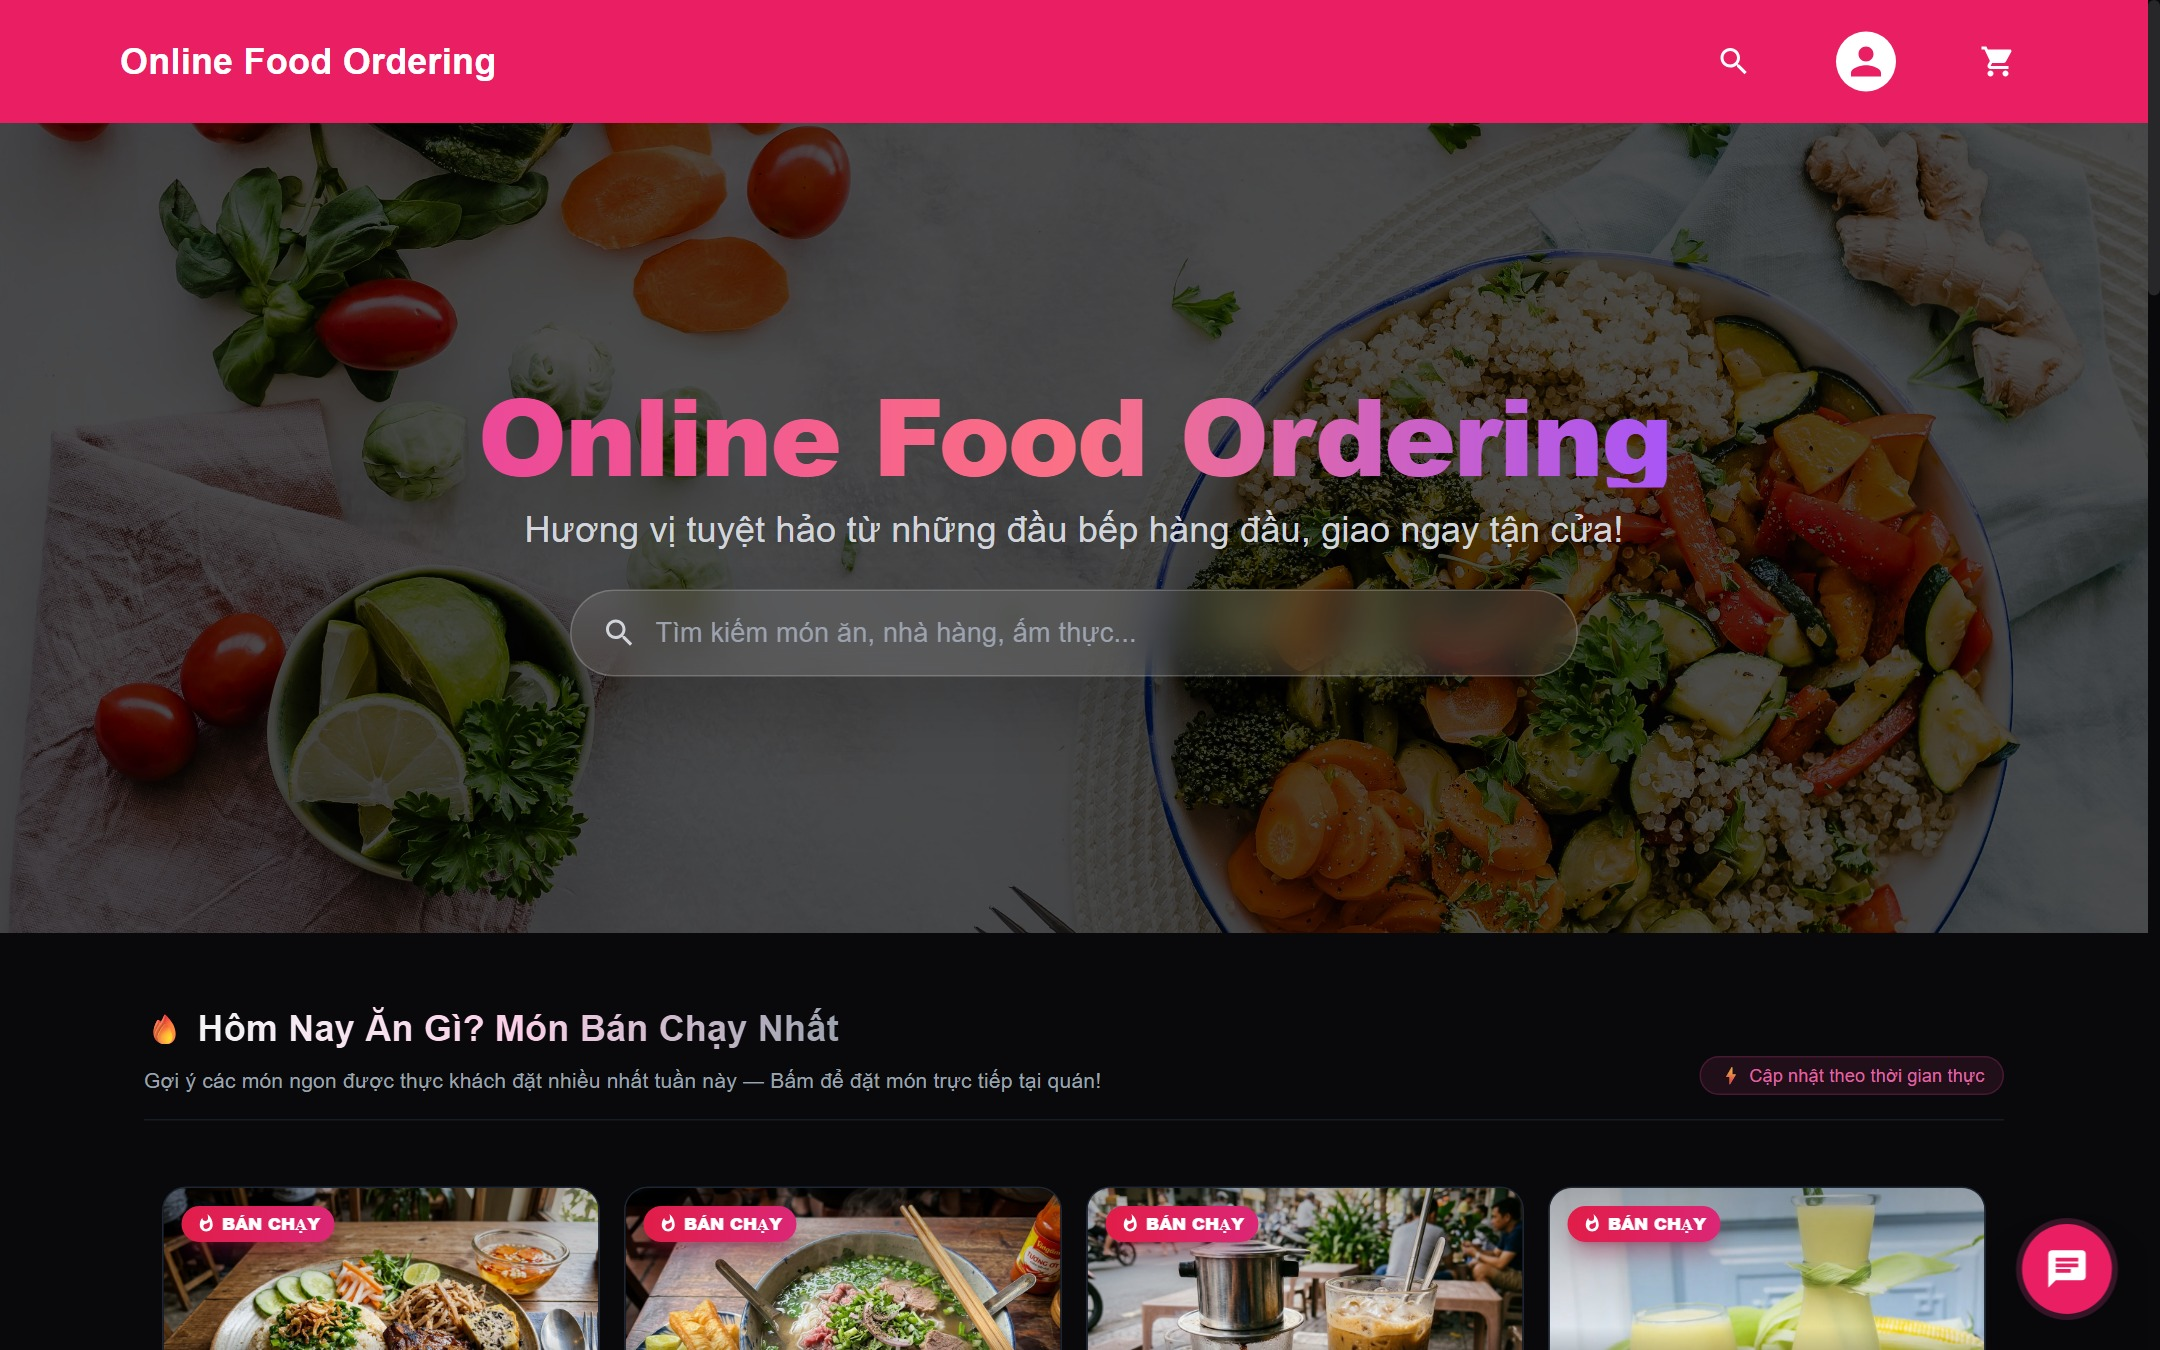
\includegraphics[width=0.95\textwidth]{figures/fig_ui_home.jpg}
\end{figure}

Hình 5.1 là ảnh chụp thực tế giao diện Dark Mode của ứng dụng: Phía trên là thanh điều hướng (Navbar) màu hồng nhận diện thương hiệu cùng các nút tìm kiếm, đăng nhập/hồ sơ và giỏ hàng. Khu vực Banner nổi bật với tiêu đề thương hiệu và thanh tìm kiếm thông minh hỗ trợ cả khách vãng lai (Guest Browsing). Ngay bên dưới là Carousel ``Hôm Nay Ăn Gì? Món Bán Chạy Nhất'' hiển thị hình ảnh chân thực của các đặc sản Việt Nam (Cơm sườn bì chả, Phở bò Bát Đàn, Cà phê phin...) cùng lưới 4 cột khám phá 16 nhà hàng và các thẻ mã giảm giá kích hoạt 1-Click.

\subsection{Màn hình Giỏ hàng và Thanh toán Đa phương thức (Cart \& Checkout Screen)}
Giao diện quản lý giỏ hàng và chốt đơn được minh họa trong Hình 5.2:

\begin{figure}{Giao diện Giỏ hàng, Gợi ý Mã Ưu đãi 1-Click và Lựa chọn Thanh toán Stripe/COD}
\centering
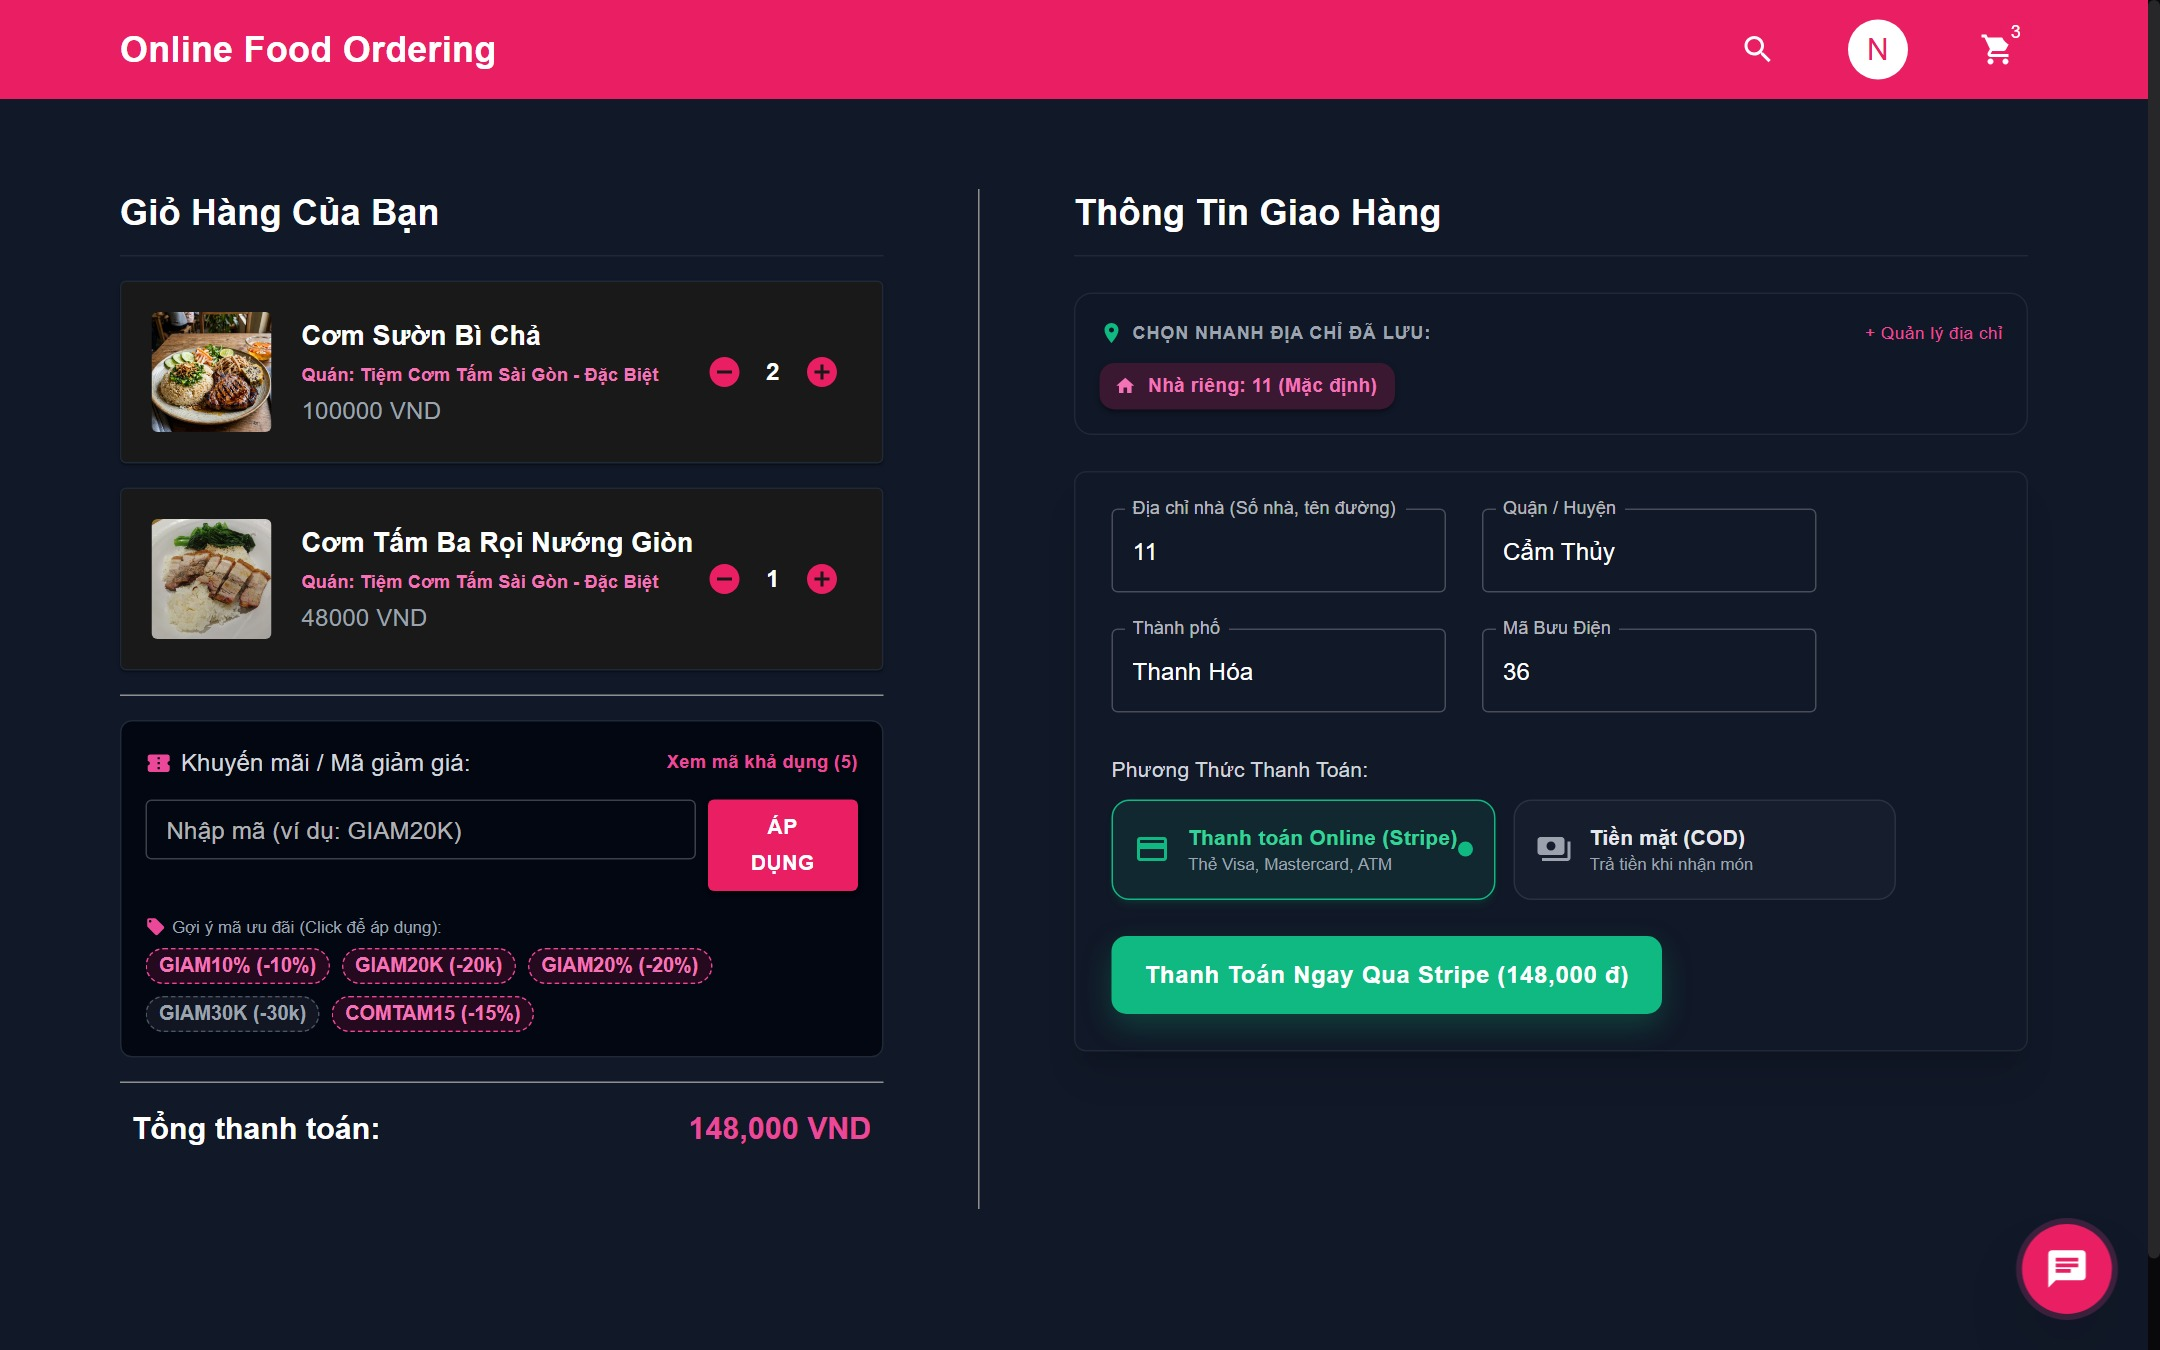
\includegraphics[width=0.95\textwidth]{figures/fig_ui_cart.jpg}
\end{figure}

Hình 5.2 thể hiện màn hình Giỏ hàng thực tế: Cột bên trái liệt kê các món ăn kèm giá tiền (ví dụ: Cơm Sườn Bì Chả, Cơm Tấm Ba Rọi Nướng Giòn), nút điều chỉnh số lượng và hộp ``Khuyến mãi / Mã giảm giá'' kèm 5 chip gợi ý áp dụng nhanh 1-Click (\texttt{GIAM10\%}, \texttt{GIAM20K}, \texttt{COMTAM15}...). Cột bên phải cho phép chọn nhanh địa chỉ giao nhận đã lưu và lựa chọn phương thức thanh toán giữa \textbf{Thanh toán Online (Stripe)} hoặc \textbf{Tiền mặt (COD)} trước khi xác nhận đặt hàng.

\subsection{Bảng Điều khiển Quản trị Nhà hàng (Restaurant Owner Dashboard)}
Giao diện dành cho đối tác chủ quán ăn được mô tả trong Hình 5.3:

\begin{figure}{Giao diện Bảng điều khiển Quản trị của Chủ nhà hàng (Real-time Dashboard)}
\centering
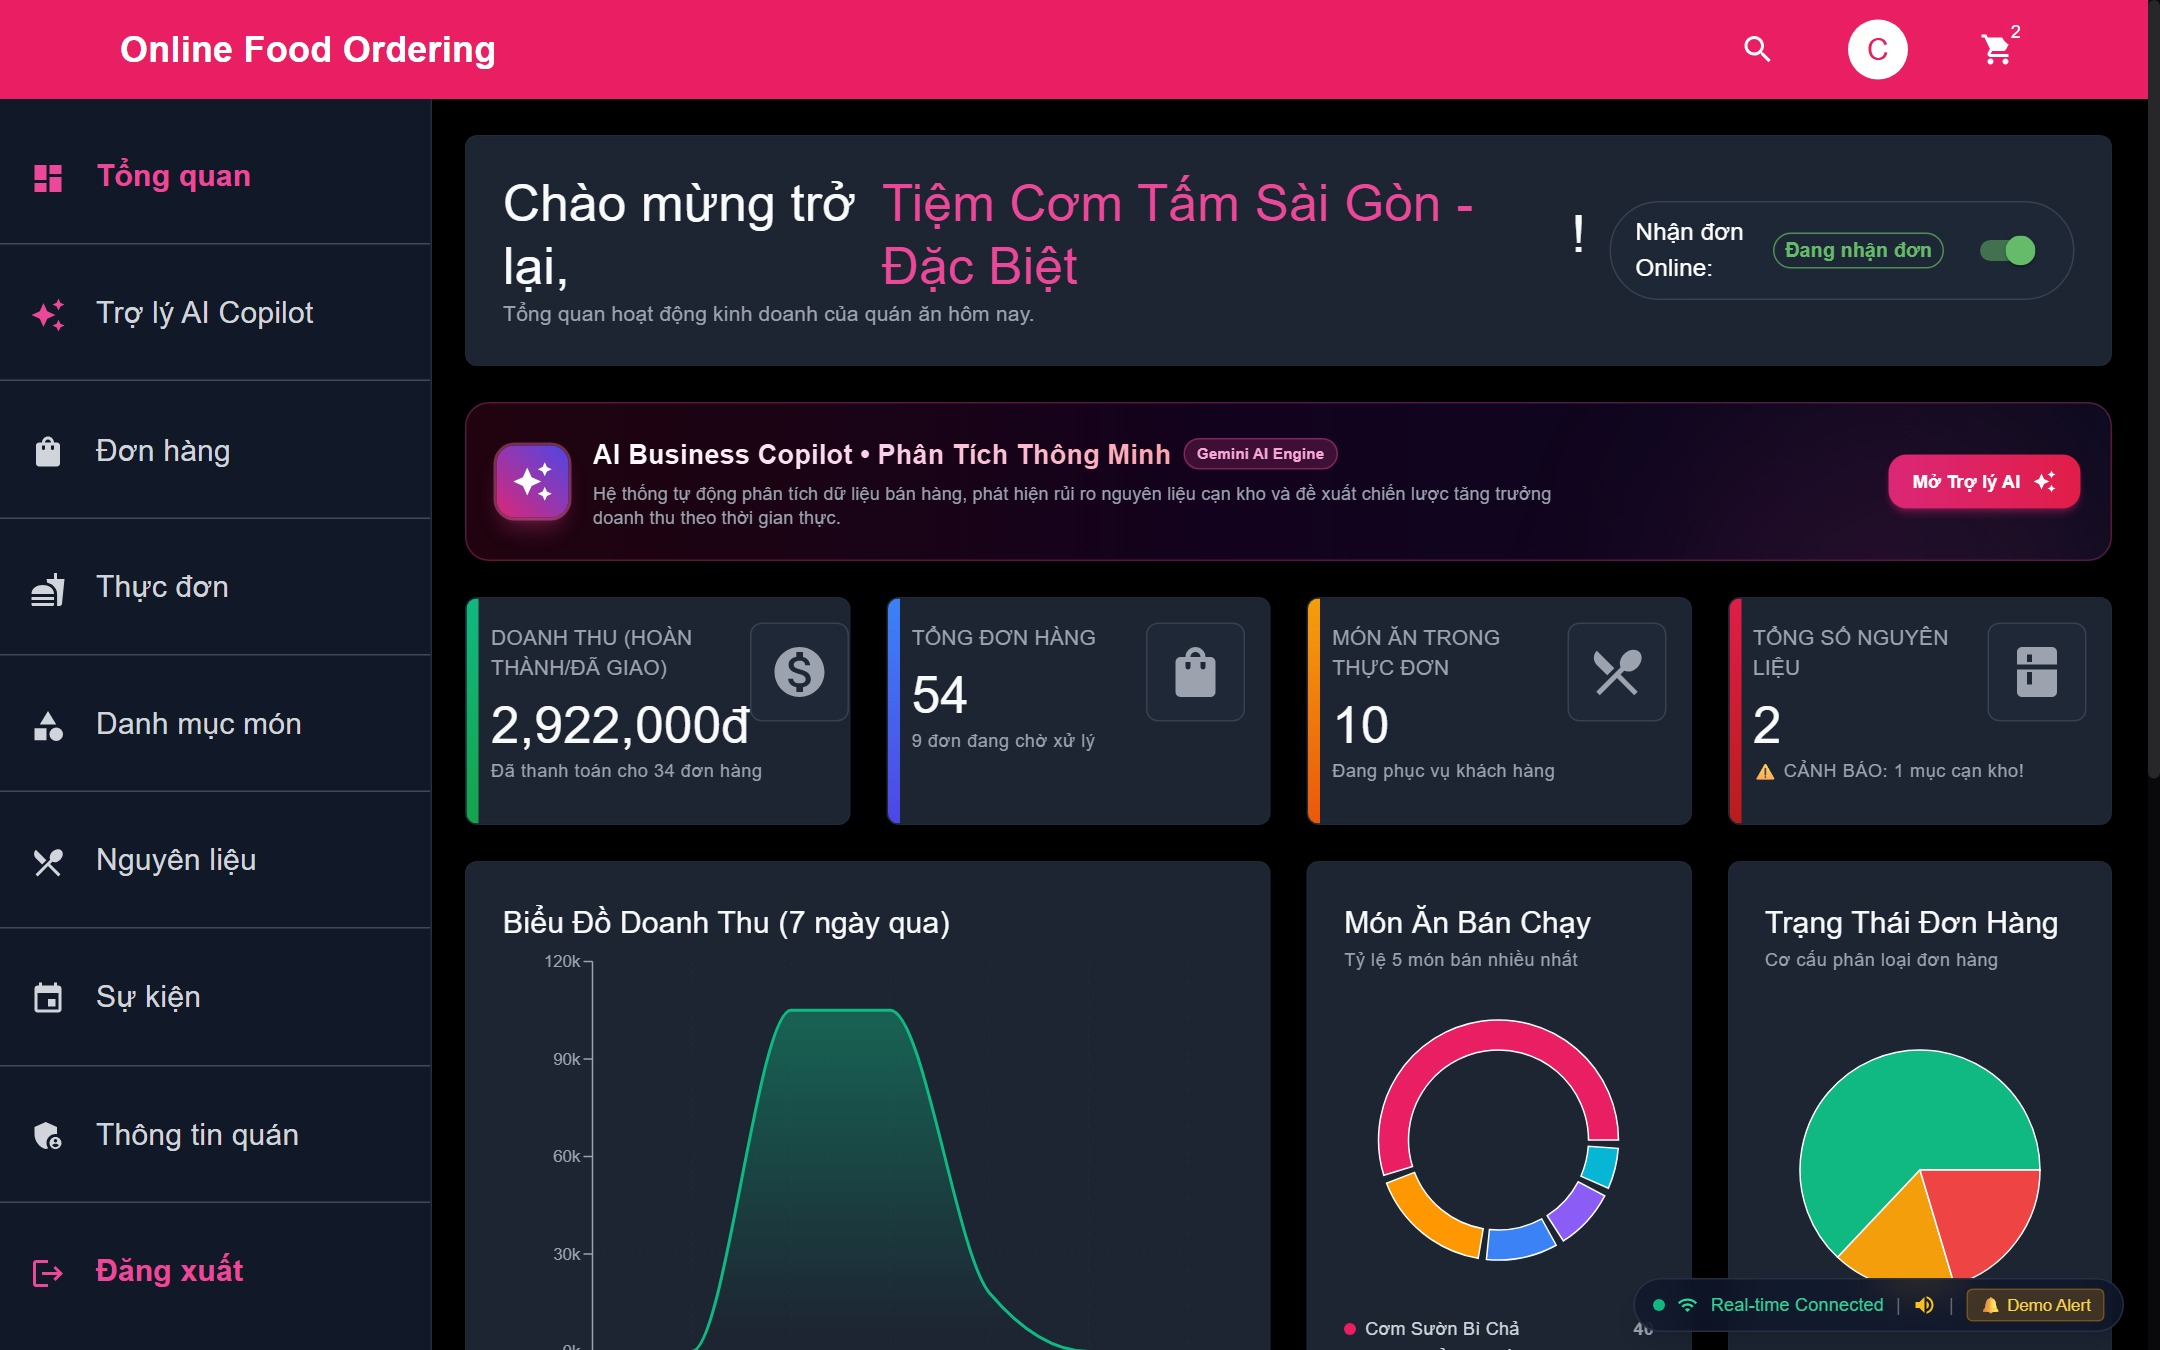
\includegraphics[width=0.95\textwidth]{figures/fig_ui_owner_dashboard.jpg}
\end{figure}

Hình 5.3 minh họa bảng điều khiển thực tế của chủ nhà hàng (\textit{Tiệm Cơm Tấm Sài Gòn - Đặc Biệt}): Bên trái là thanh Sidebar cố định hài hòa dưới Navbar gồm đầy đủ các phân hệ nghiệp vụ (\textit{Tổng quan, Trợ lý AI Copilot, Đơn hàng, Thực đơn, Danh mục món, Nguyên liệu, Sự kiện, Thông tin quán}). Khu vực nội dung hiển thị công tắc trạng thái mở nhận đơn Online, thẻ liên kết nhanh AI Business Copilot, 4 thẻ KPI thời gian thực (Doanh thu \texttt{2,922,000đ}, 54 đơn hàng, 10 món ăn, cảnh báo nguyên liệu cạn kho), các biểu đồ doanh thu 7 ngày và cơ cấu đơn hàng vẽ bằng Recharts, cùng chỉ báo WebSocket ``Real-time Connected'' ở góc dưới màn hình.

\subsection{Bảng Điều khiển Kiểm duyệt Đánh giá Toàn sàn của Super Admin}
Giao diện dành riêng cho quản trị viên tối cao sàn thương mại được mô tả trong Hình 5.4:

\begin{figure}{Giao diện Quản lý và Kiểm duyệt Đánh giá Toàn sàn của Super Admin}
\centering
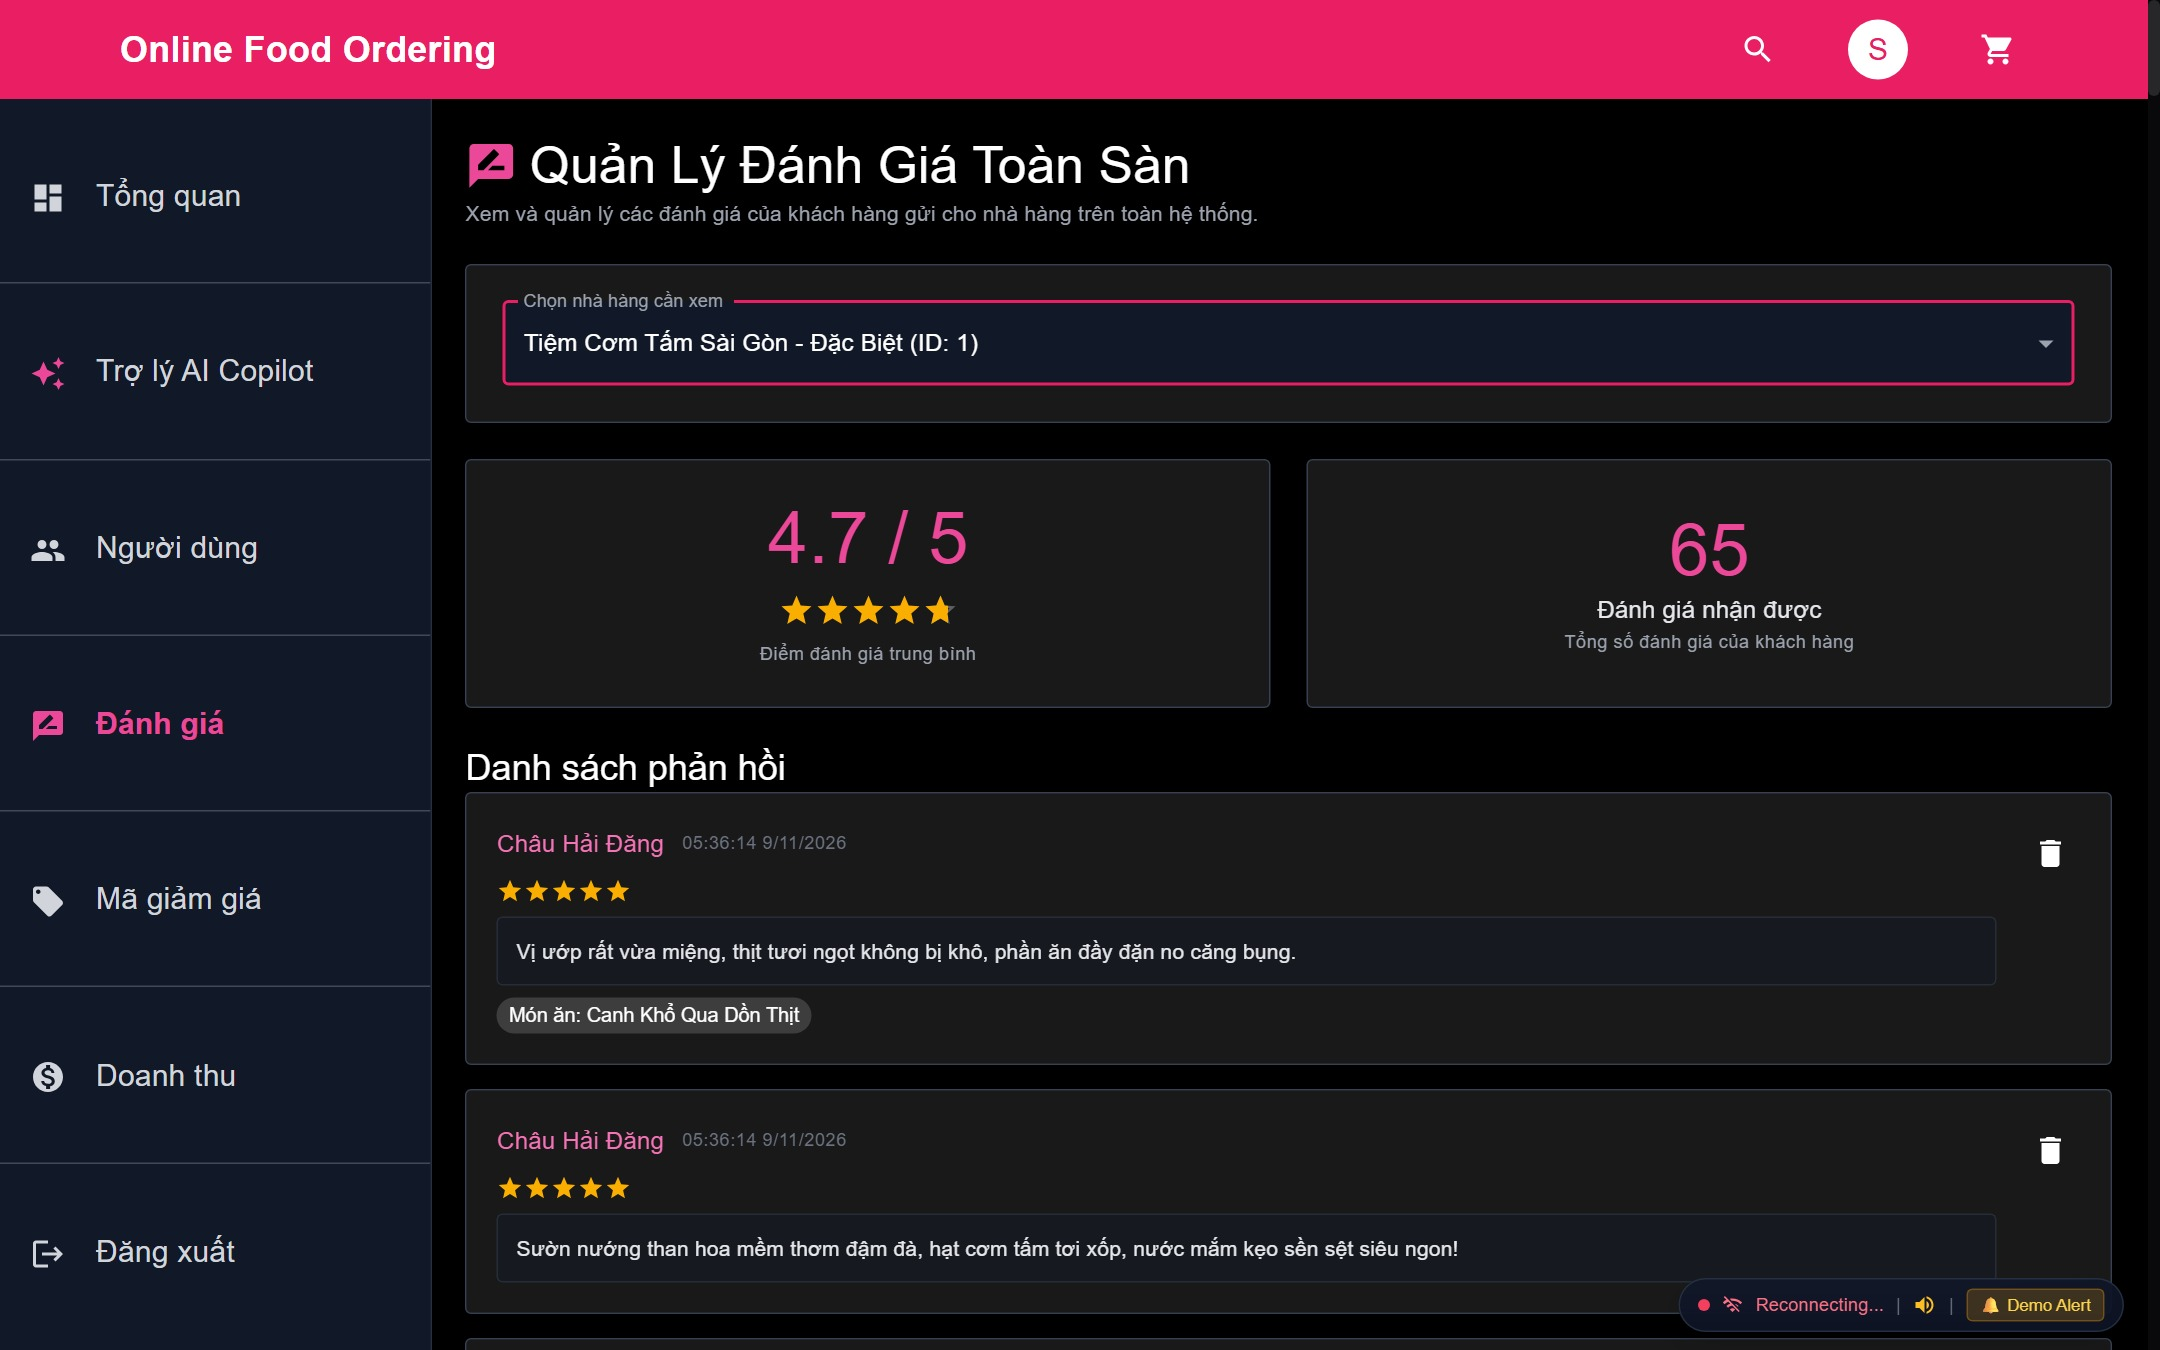
\includegraphics[width=0.95\textwidth]{figures/fig_ui_superadmin.jpg}
\end{figure}

Hình 5.4 ghi nhận phân hệ kiểm duyệt của Super Admin: Thanh Sidebar bên trái cung cấp các mục điều hành cấp sàn (\textit{Tổng quan, Trợ lý AI Copilot, Người dùng, Đánh giá, Mã giảm giá, Doanh thu}). Giao diện cho phép lọc chọn từng nhà hàng đối tác trên toàn sàn (ví dụ: \textit{Tiệm Cơm Tấm Sài Gòn - Đặc Biệt (ID: 1)}), thống kê điểm trung bình (4.7/5 sao, 65 lượt đánh giá) và liệt kê chi tiết các bình luận kèm nhãn \texttt{Chip} tên món ăn được nhận xét cùng nút gỡ bỏ các đánh giá vi phạm quy chuẩn cộng đồng.

\subsection{Màn hình Trợ lý Quản trị \& Tác tử Hành động AI Copilot}
Giao diện trợ lý AI chuyên biệt cho quản trị viên được minh họa trong Hình 5.5:

\begin{figure}{Giao diện Trợ lý Quản trị AI Copilot và Thẻ Tác tử Hành động 1-Click}
\centering
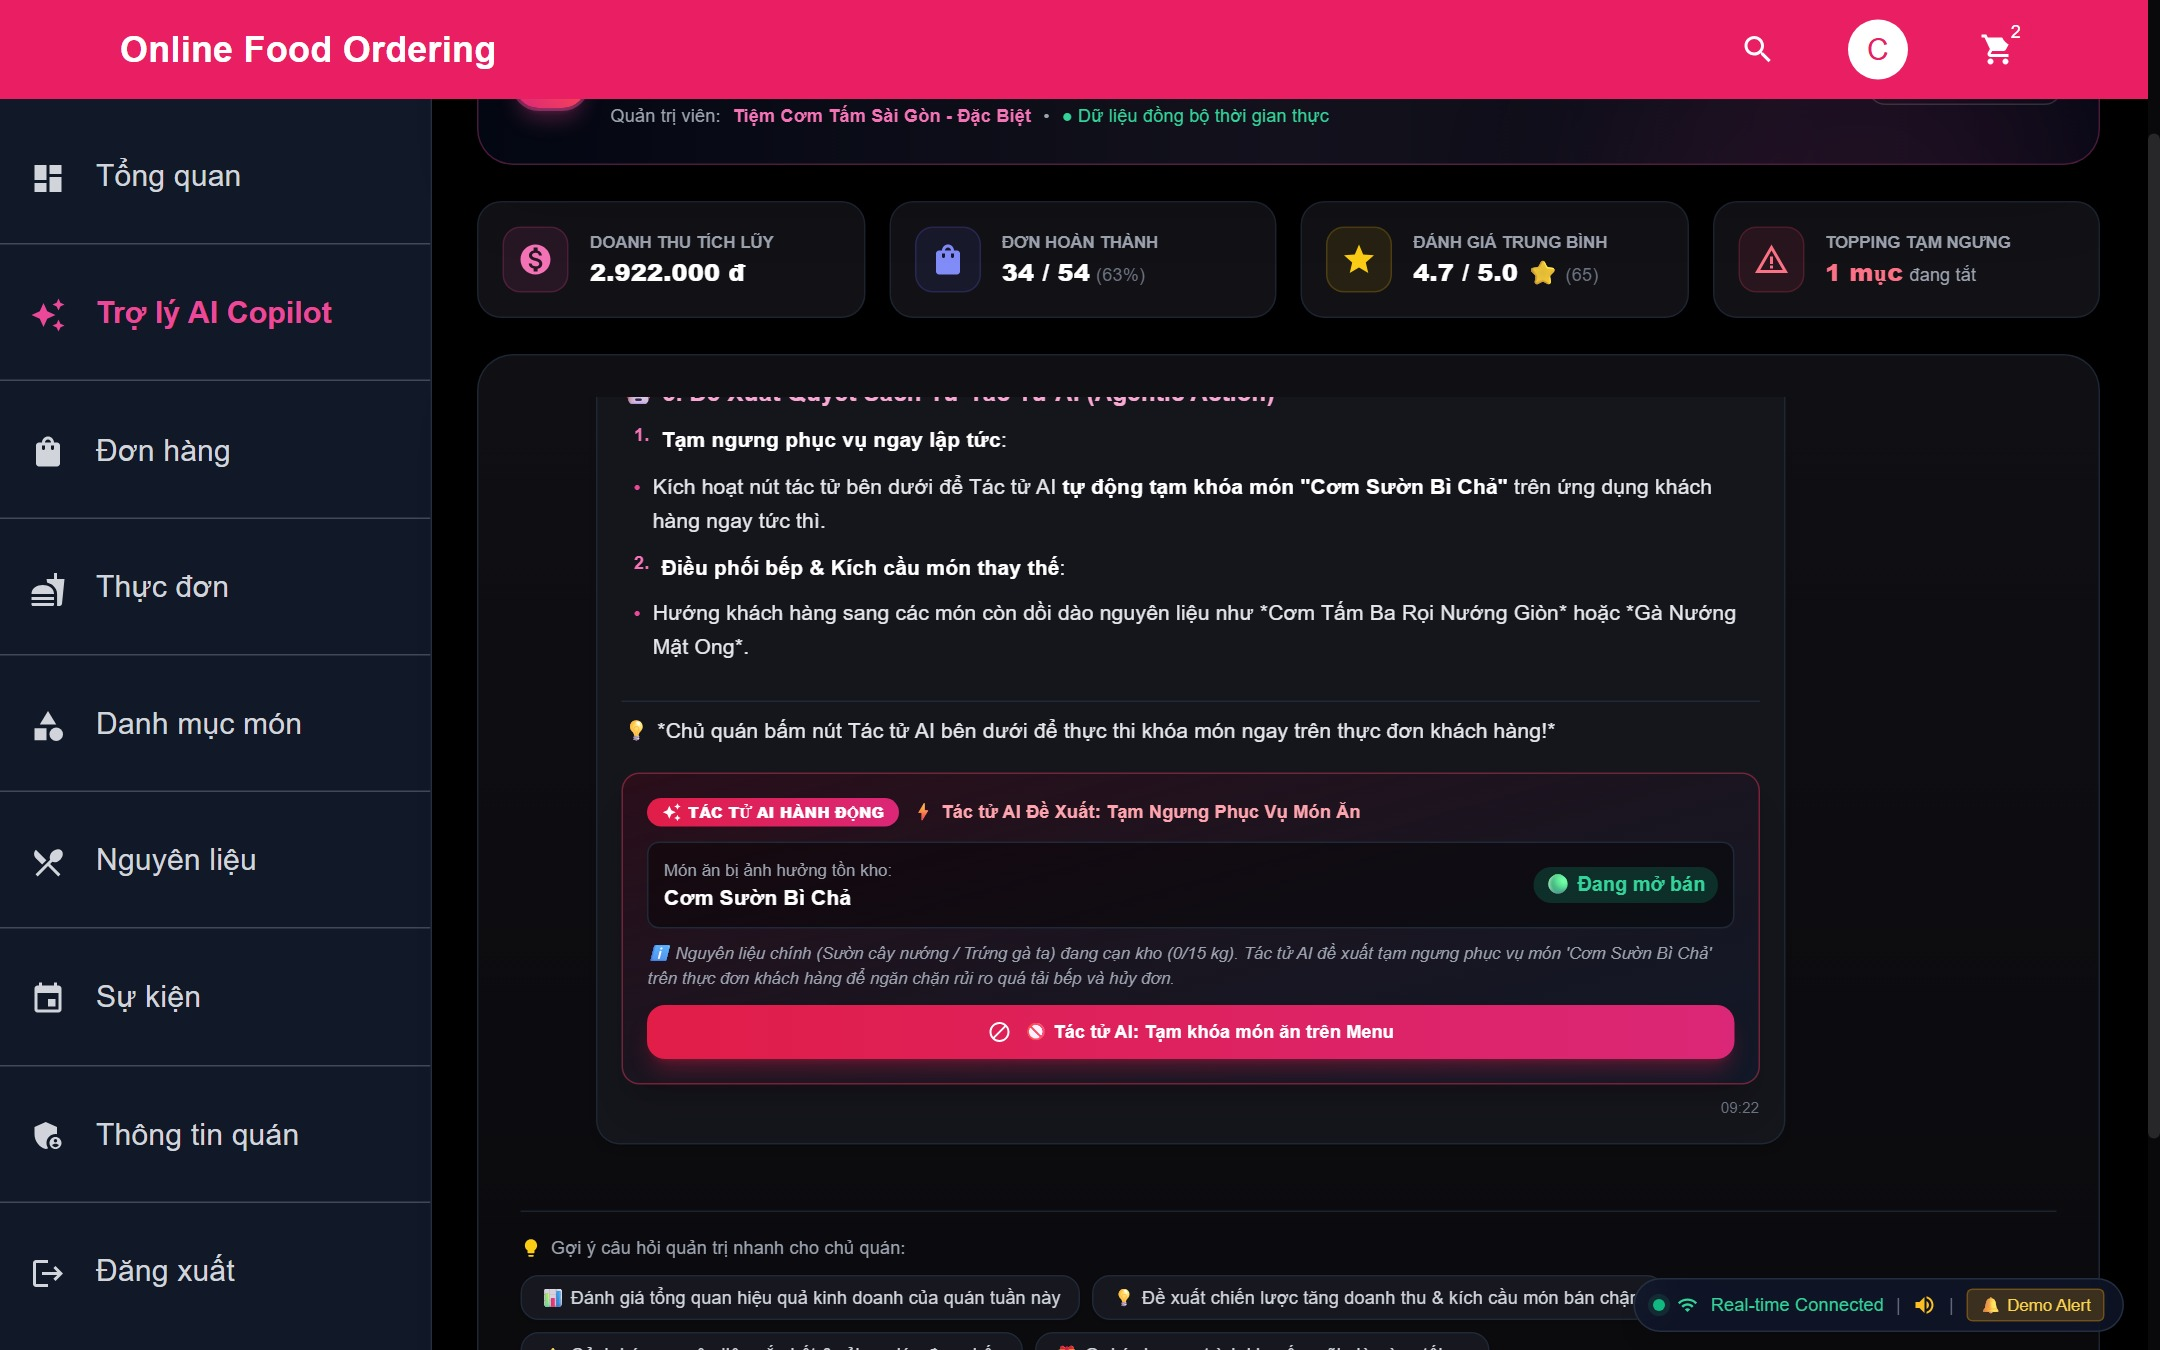
\includegraphics[width=0.95\textwidth]{figures/fig_ui_ai_copilot.jpg}
\end{figure}

Hình 5.5 cho thấy màn hình \textbf{AI Business Copilot} đang vận hành thực tế: Phía trên là hàng 4 thẻ KPI đồng bộ tức thời từ MySQL (Doanh thu tích lũy \texttt{2.922.000 đ}, 34/54 đơn hoàn thành, điểm đánh giá \texttt{4.7/5.0}, cảnh báo \texttt{1 mục đang tắt}). Khu vực trung tâm hiển thị phân tích chi tiết định dạng Markdown kết hợp nổi bật là thẻ \textbf{``TÁC TỬ AI HÀNH ĐỘNG''} đề xuất tạm ngưng phục vụ món \textit{Cơm Sườn Bì Chả} do cạn nguyên liệu sườn cây, cung cấp nút hành động trực tiếp \textit{``Tác tử AI: Tạm khóa món ăn trên Menu''} để chủ quán thực thi ngay chỉ với 1 lần nhấn.

\subsection{Giao diện Trợ lý Ẩm thực Khách hàng AI Concierge (Menu Catalog RAG)}
Giao diện Widget Chatbot thông minh phục vụ khách hàng được minh họa trong Hình 5.6:

\begin{figure}{Giao diện Trợ lý Ẩm thực Khách hàng AI Concierge với Thẻ Gợi ý Menu Catalog RAG}
\centering
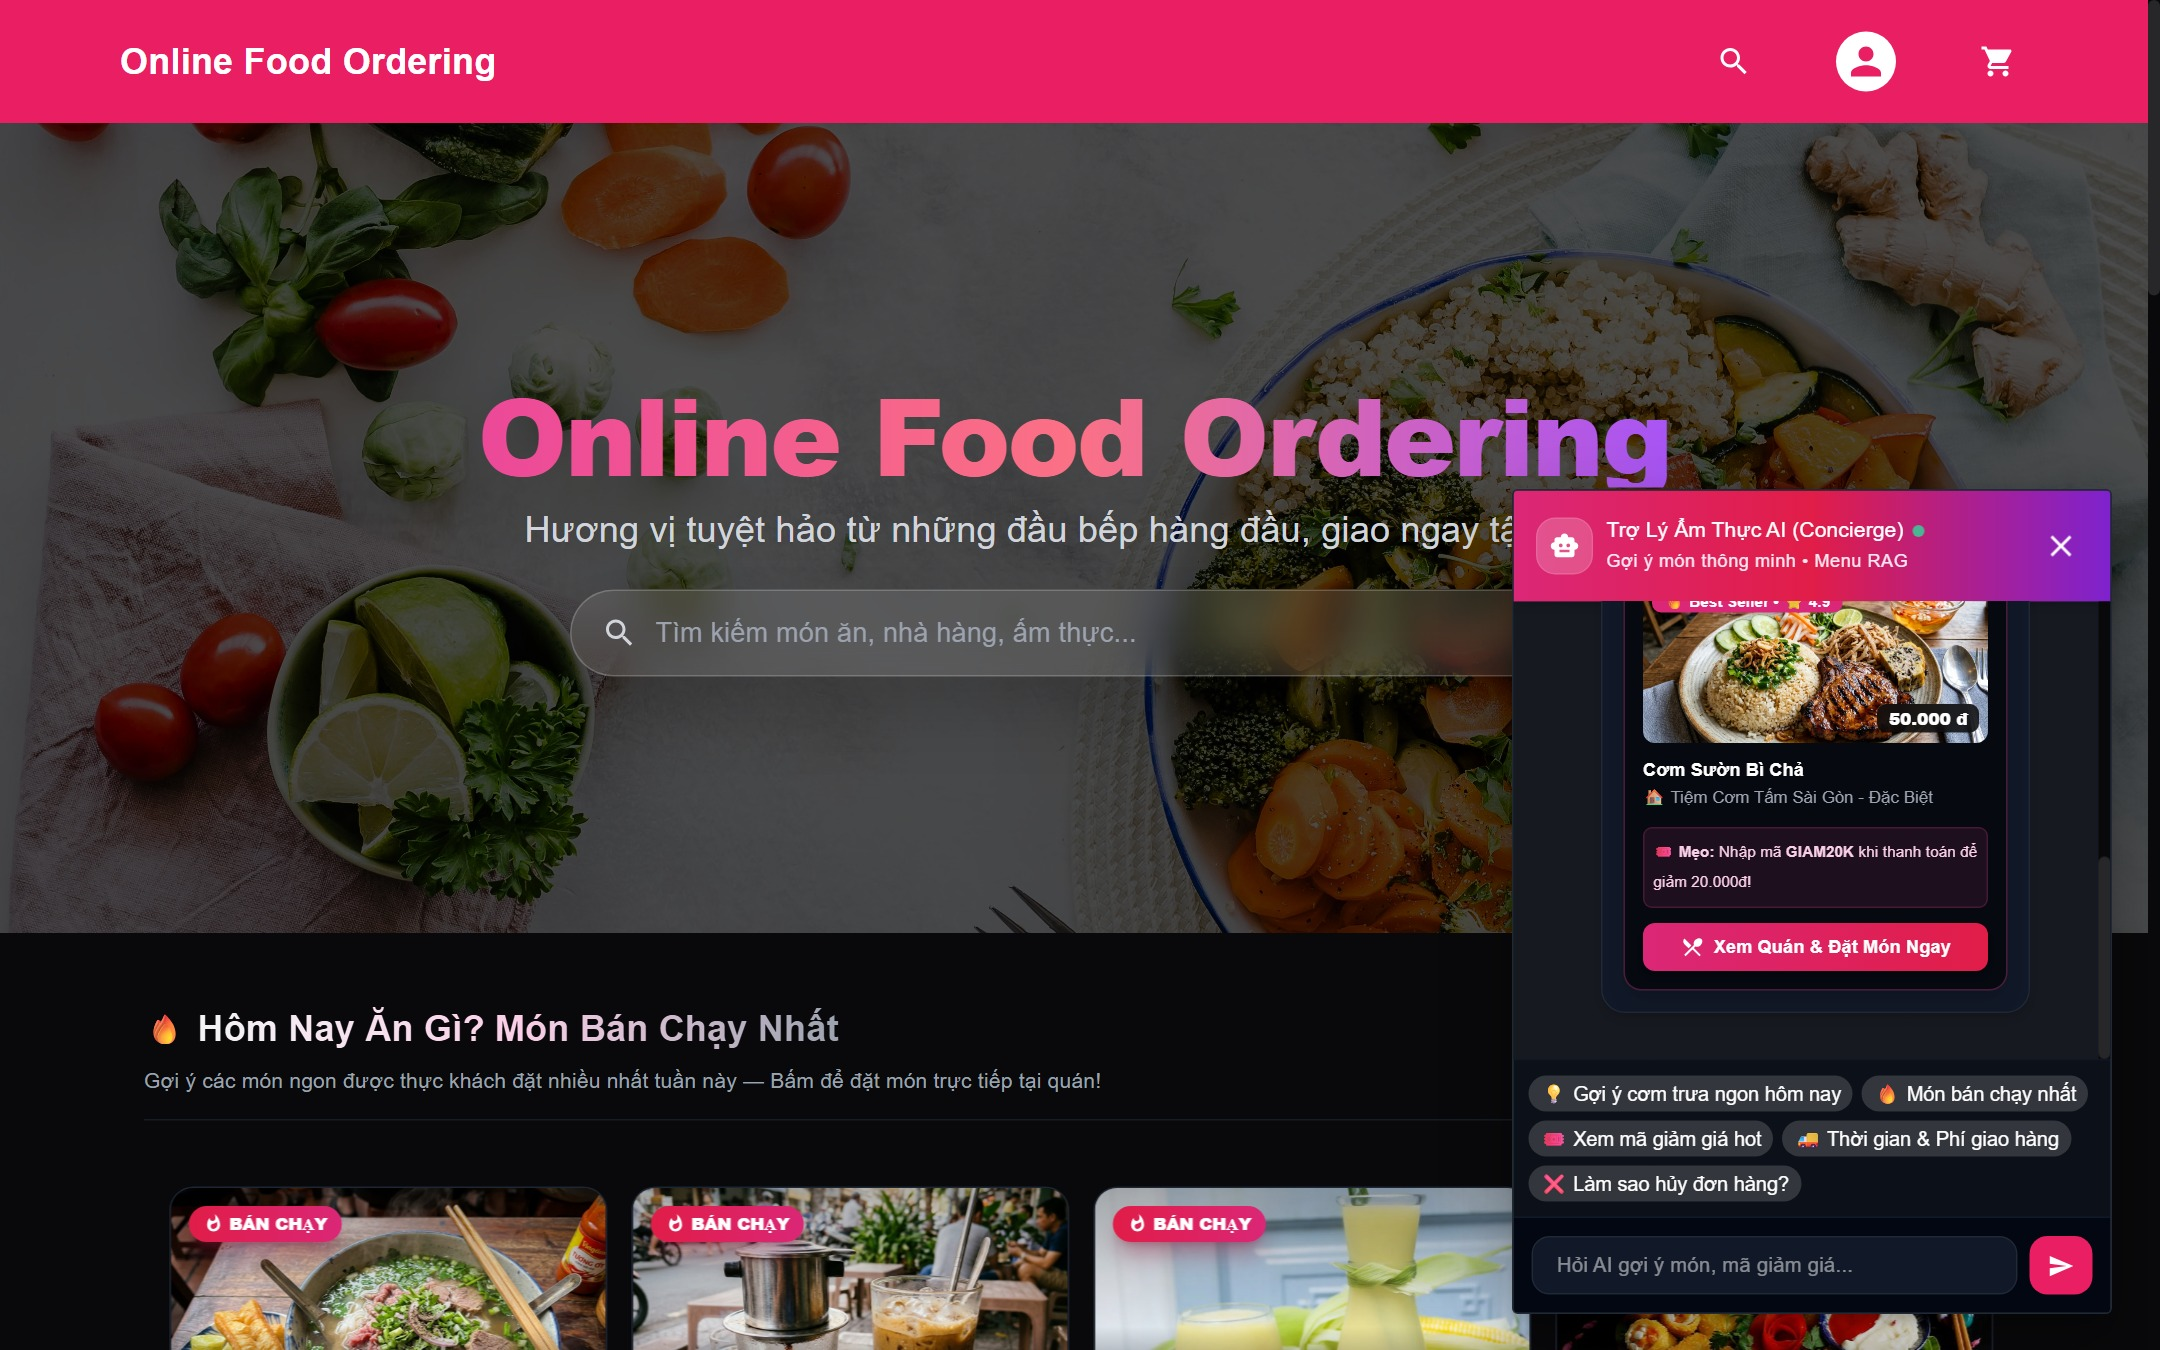
\includegraphics[width=0.95\textwidth]{figures/fig_ui_chatbot_rag.jpg}
\end{figure}

Hình 5.6 minh họa cửa sổ nổi \textbf{Trợ Lý Ẩm Thực AI (Concierge)}: Ngay khi khách hàng bấm nút gợi ý \textit{``Gợi ý cơm trưa ngon hôm nay''}, bộ truy xuất Menu Catalog RAG kết xuất trực tiếp thẻ món ăn \textit{Cơm Sườn Bì Chả (50.000 đ)} kèm ảnh thực tế, tên quán, mẹo áp dụng mã \texttt{GIAM20K} và nút tương tác \textit{``Xem Quán \& Đặt Món Ngay''} dẫn thẳng tới thực đơn nhà hàng.

% =========================================================================
% CHƯƠNG 6: KẾT LUẬN VÀ HƯỚNG PHÁT TRIỂN
% =========================================================================
\chapter{KẾT LUẬN VÀ HƯỚNG PHÁT TRIỂN}

\section{Kết luận và Đánh giá Kết quả đạt được}
\subsection{Các Kết quả Đã Hoàn thành}
Khóa luận tốt nghiệp với đề tài \textbf{``Nghiên cứu và phát triển nền tảng thương mại điện tử F\&B tích hợp quản trị thông minh''} đã hoàn thành xuất sắc toàn bộ các mục tiêu nghiên cứu và yêu cầu kỹ thuật đã đề ra ban đầu:
\begin{enumerate}
    \item \textbf{Xây dựng hoàn chỉnh kiến trúc ứng dụng Full-Stack hiện đại:} Hiện thực thành công hệ thống kết hợp giữa Java 17, Spring Boot 3.4.0 ở phía Backend và React 19, Redux Toolkit, Vite 8 ở phía Frontend. Hệ thống đạt độ gắn kết cao, hỗ trợ duyệt khám phá không cần đăng nhập (Guest Browsing) và cơ chế tự dọn dẹp token hết hạn an toàn.
    \item \textbf{Hiện thực hóa cơ chế bảo mật và phân quyền đa tầng chặt chẽ:} Ứng dụng thành công Spring Security kết hợp JSON Web Token (JWT) cho xác thực phi trạng thái; triển khai cơ chế băm mật khẩu BCrypt và chính sách chặn triệt để leo thang đặc quyền quản trị viên từ các API công khai.
    \item \textbf{Phát triển Động cơ kiểm soát mã giảm giá (Coupon Engine) \& Đồng bộ Sự kiện:} Giải quyết trọn vẹn bài toán khuyến mãi đa cấp độ (4 mã toàn sàn, 4 mã riêng nhà hàng tự động đồng bộ từ 4 sự kiện khuyến mãi); triển khai cơ chế tự động gỡ bỏ mã (Auto-removal) tại giao diện và thuật toán kiểm tra an toàn biên (\texttt{Math.max}, \texttt{Math.min}) tại máy chủ.
    \item \textbf{Tích hợp Thanh toán Đa phương thức (Stripe Checkout \& COD) và Máy trạng thái Đơn hàng:} Xây dựng luồng thanh toán thẻ quốc tế Stripe chuẩn PCI DSS (với callback mở khóa an toàn), hỗ trợ song song thanh toán COD và xuất hóa đơn điện tử; thiết lập \textbf{Order State Guard} ngăn chuyển trạng thái trái quy trình.
    \item \textbf{Hiện thực hóa truyền thông đơn hàng thời gian thực qua WebSocket \& Chuông thuật toán:} Loại bỏ hoàn toàn cơ chế kéo định kỳ HTTP Polling, đưa độ trễ nhận đơn hàng xuống còn 26,5ms (nhanh gấp 57,6 lần), luôn sắp xếp đơn hàng mới nhất lên đầu và tích hợp chuông âm thanh Web Audio API.
    \item \textbf{Xây dựng Hệ sinh thái AI Đa tầng (Dual-Persona Agentic AI Copilot \& Menu Catalog RAG Chatbot):} Kết hợp \textbf{Google Gemini 2.5 Flash} và Động cơ Heuristic DSS dự phòng hai tầng (đạt độ sẵn sàng 100\%) kèm tính năng Tác tử AI 1-Click khóa món cạn kho/gỡ đánh giá vi phạm cho quản trị viên, cùng Widget Chatbot Menu Catalog RAG hỗ trợ thực khách đặt món nhanh qua deep-link.
    \item \textbf{Phát triển phân hệ Quản lý Kho nguyên liệu Tự động (Smart Stock Depletion Engine):} Tự động khấu trừ và hoàn trả tồn kho nguyên liệu theo từng đơn hàng phát sinh hoặc bị hủy (bao gồm lúc chủ quán chuyển trạng thái hủy), ghi vết minh bạch vào nhật ký biến động kho \texttt{InventoryLog} với độ lệch tồn kho bằng 0\%.
    \item \textbf{Thiết kế cơ sở dữ liệu chuẩn hóa và Hệ sinh thái dữ liệu thực tế:} Xây dựng mô hình ERD gồm 21 bảng chuẩn 3NF, bảo đảm tính toàn vẹn ACID cùng bộ dữ liệu thử nghiệm chuẩn thực tiễn (16 nhà hàng thuộc 3 thành phố, 82 món ăn ảnh thật, kịch bản khởi tạo tự động và bản sao lưu SQL \texttt{restore\_images\_and\_coupons.sql}).
    \item \textbf{Trải nghiệm người dùng vượt trội với Dark Mode UI:} Thiết kế giao diện đồng bộ, mượt mà trên Material-UI 9, Recharts và TailwindCSS, tối ưu hóa thao tác với lưới 4 cột thích ứng, Carousel ``Hôm nay ăn gì?'', đánh giá theo từng món và thanh điều hướng quản trị nhất quán.
\end{enumerate}

\subsection{Đánh giá Ưu điểm Nổi bật của Hệ thống}
\begin{itemize}
    \item \textbf{Tính thực tiễn và sẵn sàng triển khai cao:} Không chỉ dừng lại ở mức mô hình nghiên cứu lý thuyết, hệ thống đã giải quyết trọn vẹn các bài toán nghiệp vụ gai góc trong thực tế của ngành F\&B như: tùy biến nguyên liệu theo món, thanh toán thẻ quốc tế thực tế, cơ chế hủy đơn an toàn, kiểm duyệt đánh giá xấu, cảnh báo đơn hàng tức thời, quản trị kho tự động và phân tích kinh doanh bằng AI.
    \item \textbf{Kiến trúc mã nguồn rõ ràng, dễ bảo trì:} Codebase được tổ chức theo cấu trúc phân tầng chuẩn mực (Controller, Service, Repository, DTO, Redux Slices, Components), tuân thủ nguyên lý thiết kế SOLID và các quy ước kỹ thuật chuẩn của cộng đồng Spring và React.
    \item \textbf{Bảo mật và an toàn dữ liệu cao:} Đảm bảo kiểm tra quyền truy cập ở từng endpoint, bảo vệ dữ liệu thẻ khách hàng và loại trừ các lỗ hổng bảo mật phổ biến.
\end{itemize}

\section{Hạn chế Hiện tại của Hệ thống}
Bên cạnh những kết quả tích cực đã đạt được, hệ thống vẫn tồn tại một số hạn chế nhất định do giới hạn về mặt thời gian và nguồn lực nghiên cứu:
\begin{itemize}
    \item \textbf{Chưa có phân hệ định vị GPS cho người giao hàng (Shipper tracking):} Hệ thống hiện mới tập trung vào mối quan hệ giữa Khách hàng, Chủ quán và Quản trị sàn; quy trình điều phối đội ngũ giao hàng vật lý trên bản đồ số chưa được tích hợp trực tiếp.
    \item \textbf{Phương thức thanh toán trực tuyến nội địa còn hạn chế:} Mới tích hợp cổng thanh toán quốc tế Stripe (chủ yếu cho thẻ Visa/MasterCard), chưa mở rộng kết nối tới các cổng thanh toán nội địa và ví điện tử phổ biến tại Việt Nam như VNPay-QR, MoMo, ZaloPay.
    \item \textbf{Mô hình dự báo nhu cầu bằng Machine Learning nâng cao:} Trợ lý AI hiện tại tập trung vào phân tích các chỉ số lịch sử và thời gian thực hiện tại; hệ thống chưa xây dựng mô hình học sâu chuyên sâu dự báo nhu cầu khách hàng theo chuỗi thời gian (Time-series Forecasting) có tính đến các yếu tố thời tiết hoặc ngày nghỉ lễ.
\end{itemize}

\section{Định hướng Phát triển trong Tương lai}
Nhằm nâng cấp hệ thống trở thành một nền tảng thương mại ẩm thực quy mô lớn, các hướng nghiên cứu và phát triển tiếp theo được đề xuất bao gồm:
\begin{enumerate}
    \item \textbf{Nghiên cứu mô hình Machine Learning dự báo nhu cầu nguyên liệu và món ăn (Demand Forecasting):} Huấn luyện các mô hình học sâu chuỗi thời gian (như LSTM, Prophet hoặc Temporal Fusion Transformer) dựa trên lịch sử đặt món, thời tiết và dữ liệu sự kiện để dự báo trước lượng nguyên liệu cần nhập, giảm thiểu tối đa hao hụt thực phẩm.
    \item \textbf{Mở rộng tích hợp các cổng thanh toán nội địa:} Tích hợp thêm các giải pháp thanh toán số phổ biến tại thị trường Việt Nam như VNPay-QR, MoMo Payment Gateway và ZaloPay để tạo sự thuận tiện tối đa cho người tiêu dùng trong nước.
    \item \textbf{Phát triển ứng dụng di động nguyên bản (Mobile Apps):} Xây dựng ứng dụng di động dành cho tài xế giao hàng (Shipper App) sử dụng React Native hoặc Flutter, tích hợp Google Maps API để theo dõi hành trình giao nhận theo thời gian thực.
    \item \textbf{Chuyển đổi sang kiến trúc Microservices và đóng gói Container:} Tiến hành phân rã hệ thống nguyên khối (Monolith) thành các vi dịch vụ độc lập (Auth Service, Order Service, Restaurant Service, Inventory Service, Payment Service), đóng gói bằng Docker và điều phối cụm bằng Kubernetes (K8s) trên nền tảng điện toán đám mây (AWS/GCP), sẵn sàng phục vụ hàng triệu người dùng đồng thời.
\end{enumerate}

% =========================================================================
% TÀI LIỆU THAM KHẢO
% =========================================================================
\begin{thebibliography}{99}
\begin{bibsection}{Tài liệu tiếng Việt}
\bibitem{viet1} Bộ Thông tin và Truyền thông, \textit{Báo cáo Kinh tế số Việt Nam và Xu hướng Thương mại điện tử ẩm thực giai đoạn 2024 -- 2026}, Nhà xuất bản Thông tin và Truyền thông, Hà Nội, 2024.
\bibitem{viet2} Trần Tất Việt, \textit{Nghiên cứu mã hóa đầu cuối trong ứng dụng nhắn tin}, Khóa luận tốt nghiệp đại học ngành Công nghệ thông tin, Trường Đại học Công nghệ -- Đại học Quốc gia Hà Nội, 2025.
\bibitem{viet3} Phùng Lê Anh Quân, \textit{Xây dựng mô-đun liên kết tiếp thị hỗ trợ các sàn thương mại điện tử}, Khóa luận tốt nghiệp đại học ngành Công nghệ thông tin, Trường Đại học Công nghệ -- Đại học Quốc gia Hà Nội, 2025.
\bibitem{viet4} Nguyễn Văn Vinh, \textit{Giáo trình Kỹ nghệ phần mềm và Thiết kế hệ thống thông tin hướng đối tượng}, Nhà xuất bản Đại học Quốc gia Hà Nội, 2022.
\end{bibsection}

\begin{bibsection}{Tài liệu tiếng Anh}
\bibitem{eng1} Walls, C., \textit{Spring in Action, Sixth Edition}, Manning Publications, 2022.
\bibitem{eng2} Spilca, L., \textit{Spring Security in Action, Second Edition}, Manning Publications, 2023.
\bibitem{eng3} Banks, A., \& Porcello, E., \textit{Learning React: Modern Patterns for Developing React Applications, 2nd Edition}, O'Reilly Media, 2020.
\bibitem{eng4} Redux Team, \textit{Redux Toolkit Documentation: The official, opinionated, batteries-included toolset for efficient Redux development}, Available: \url{https://redux-toolkit.js.org/}, Accessed: April 2026.
\bibitem{eng5} Stripe Inc., \textit{Stripe API Documentation \& Integration Guide for Java and React}, Available: \url{https://stripe.com/docs/api}, Accessed: April 2026.
\bibitem{eng6} Fielding, R. T., \textit{Architectural Styles and the Design of Network-based Software Architectures}, Doctoral dissertation, University of California, Irvine, 2000.
\bibitem{eng7} Silberschatz, A., Korth, H. F., \& Sudarshan, S., \textit{Database System Concepts, 7th Edition}, McGraw-Hill, 2020.
\bibitem{eng8} Rescorla, E., \textit{The Transport Layer Security (TLS) Protocol Version 1.3}, RFC 8446, Internet Engineering Task Force (IETF), 2018.
\bibitem{eng9} Martin, R. C., \textit{Clean Architecture: A Craftsman's Guide to Software Structure and Design}, Prentice Hall, 2017.
\bibitem{eng10} Jones, M., Bradley, J., \& Sakimura, N., \textit{JSON Web Token (JWT)}, RFC 7519, Internet Engineering Task Force (IETF), 2015.
\end{bibsection}
\end{thebibliography}

\end{document}
